\begin{appendix} %Anhang
\section{Matlab-Berechnungen}
\subsection{Leistungsfaktor}
\lstinputlisting{appendix/code/Leistungsfaktor.m}

\newpage
\subsection{Arduino-Programm}
\begin{lstlisting}[language=Arduino]
const int Switch_PO = 3;         // Output fuer den EIN- und AUSSCHALTER
const int Controll_P = 2;   // Output fuer Steuersignal
const int Switch_PI = 5; // Input fuer den EIN- und AUSSCHALTER
int buttonState = 0;                 // Zustand Schalter auf 0
int anzahl_Schwinwungspakete = 5;        // Anzahl Schwingungspakete

void setup() {
pinMode (Switch_PO, OUTPUT);        // Schalter auf Output
pinMode (Controll_P, OUTPUT);              // PWM auf Output
pinMode (Switch_PI, INPUT_PULLUP);      // Schalter Eingang
}

void loop() {
buttonState =! digitalRead(Switch_PI);      // Da Pullup wird das Signal negiert
if(buttonState == HIGH){          // if-Schleife falls Zustand Schalter auf EIN
for(int z=0; z<10; z++){             // for-Schleife fuer Schwingungspaketsteuerung
if(z<anzahl_Schwinwungspakete){                 // Anzahl Schwingungen EIN
for(int i=0; i<255; i++){                     // Hochfahren mit PWM
analogWrite(Controll_P, i);  // Die Variable wird auf den Steuersignalausgang geschrieben
delay(5);// Kurze Zeitverzoegerung da sonst das PWM zu schnell fuer ein Multimeter hochfaehrt       
}
delay(200);     // Warten waehrend volle Leistung
for(int i=255; i>0; i--){                     // Runterfahren mit PWM
analogWrite(Controll_P, i);                 // Die Variable wird auf den Steuersignalausgang geschrieben
delay(5); // Kurze Zeitverzoegerung da sonst das PWM zu schnell fuer ein Multimeter runterfaehrt
}
delay(100);   // Warten waehrend keiner Leistung
}else{
digitalWrite(Controll_P, LOW); // Ausschalten fuer Schwingungspakete keine Leistung
delay((10-anzahl_Schwinwungspakete)*480);     // Verzoegerung bis wieder eingeschaltet werden soll
			}
}
}
}





\end{lstlisting}

\newpage
\section{Vergleich der Resultate von Plecs und Matlab}

\begin{figure}[ht!]
	\centering
	\subfloat[][]{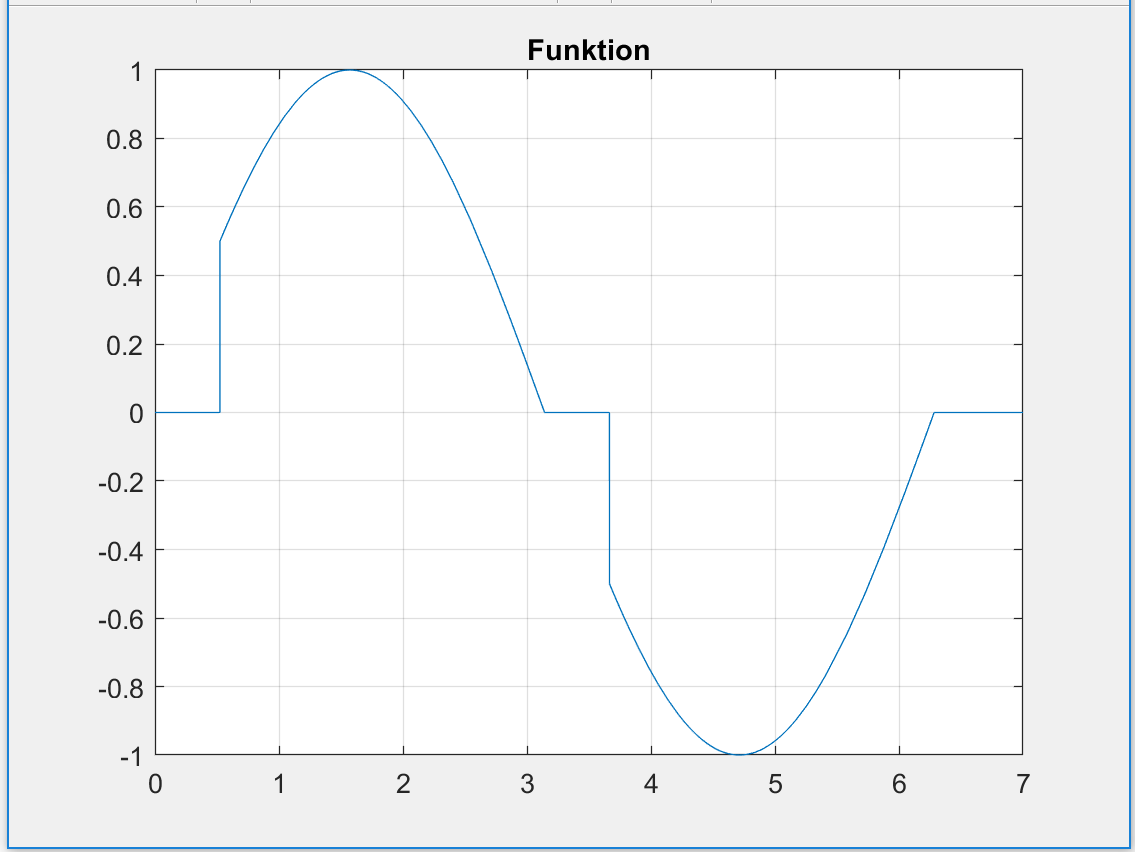
\includegraphics[width=0.4\linewidth]{eingangssignal_30.png}\label{fig:eingangssignal_30}}\qquad
	\subfloat[][]{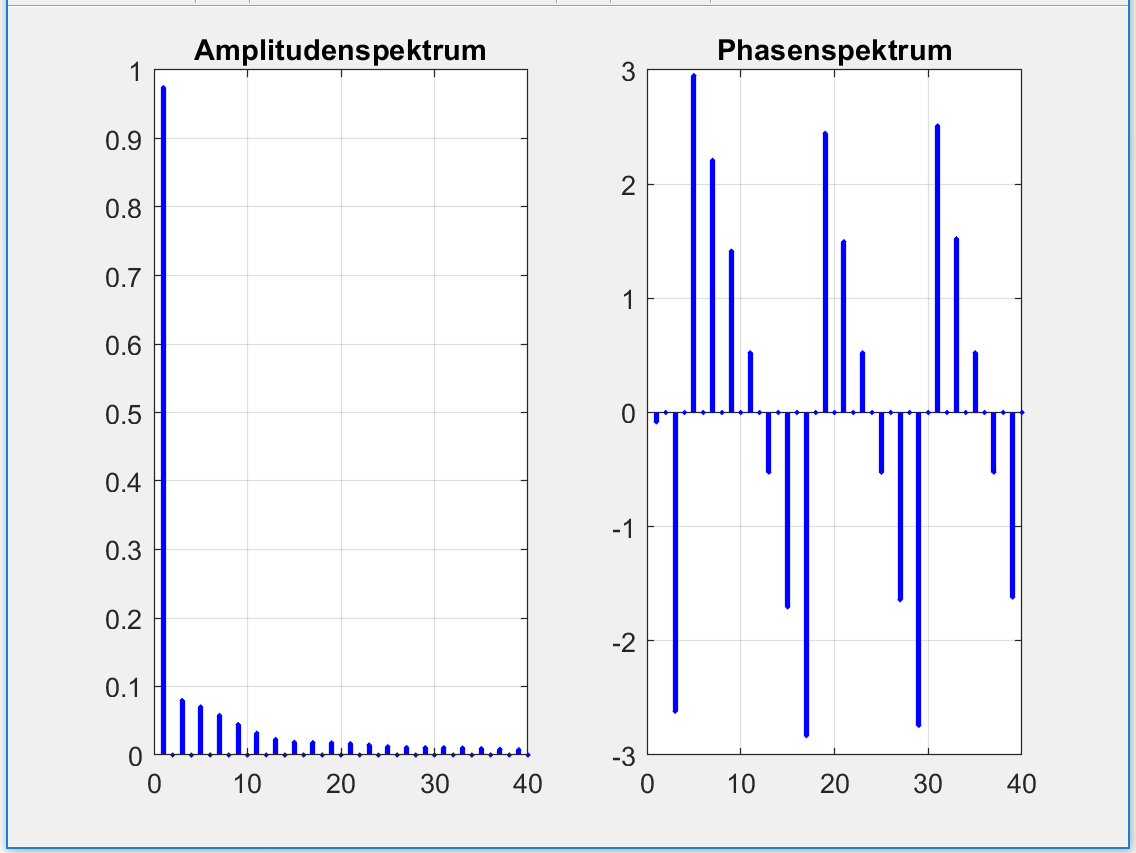
\includegraphics[width=0.4\linewidth]{A_PH_30.png}\label{fig:A_PH_30.}}
	\caption{Phasenanschnittsteuerung mit 30\textdegree (a) Eingangssignal (b) Amplituden- und Phasenspektrum}
	\label{fig:Phasenanschnittsteuerung_mit_30}
\end{figure}

\begin{figure}[ht!]
	\centering
	\subfloat[][]{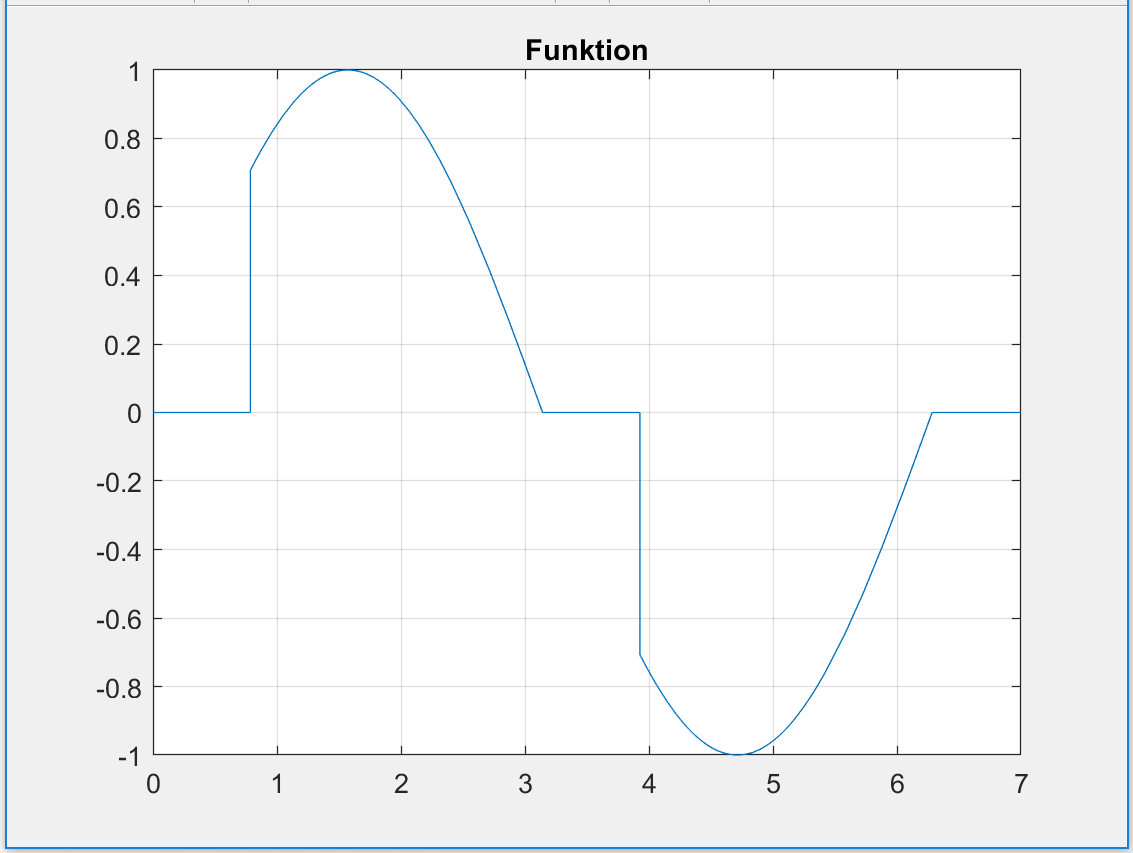
\includegraphics[width=0.4\linewidth]{eingangssignal_45.png}\label{fig:eingangssignal_45}}\qquad
	\subfloat[][]{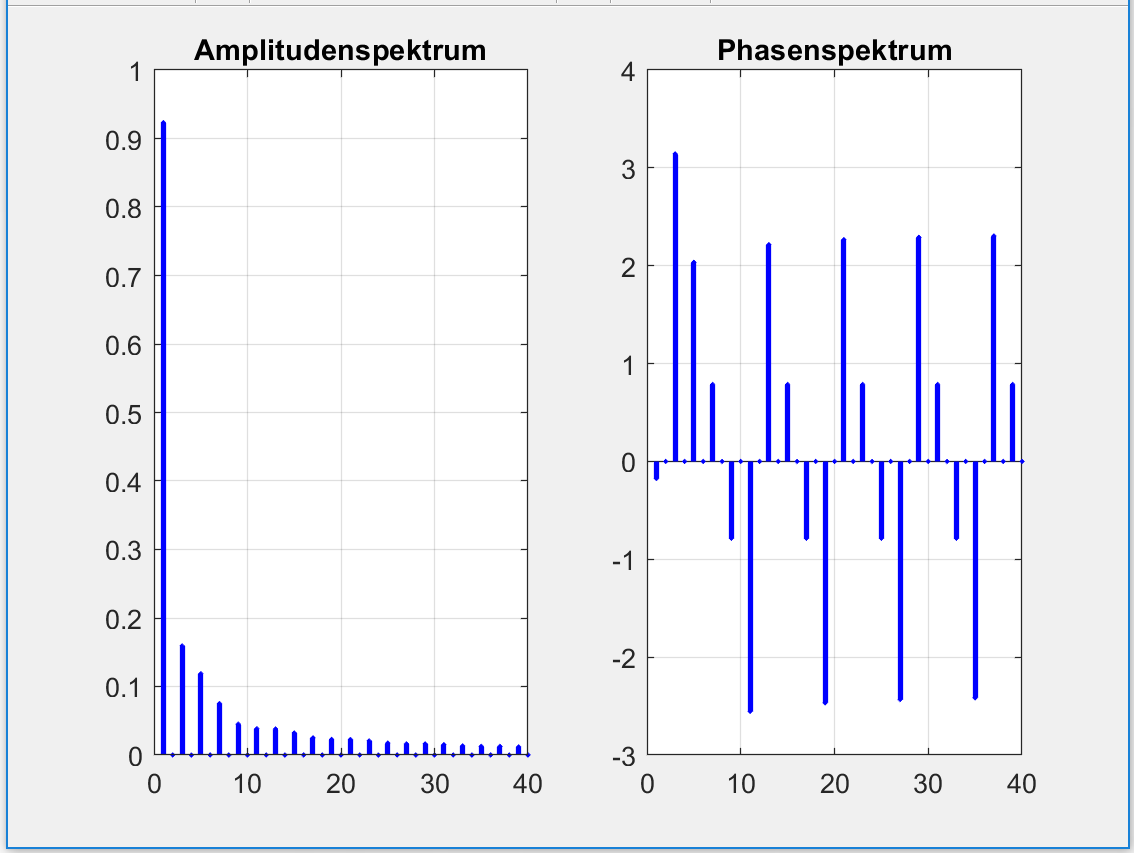
\includegraphics[width=0.4\linewidth]{A_PH_45.png}\label{fig:A_PH_45}}
	\caption{Phasenanschnittsteuerung mit 45\textdegree (a) Eingangssignal (b) Amplituden- und Phasenspektrum}
	\label{fig:Phasenanschnittsteuerung_mit_45}
\end{figure}

\begin{figure}[ht!]
	\centering
	\subfloat[][]{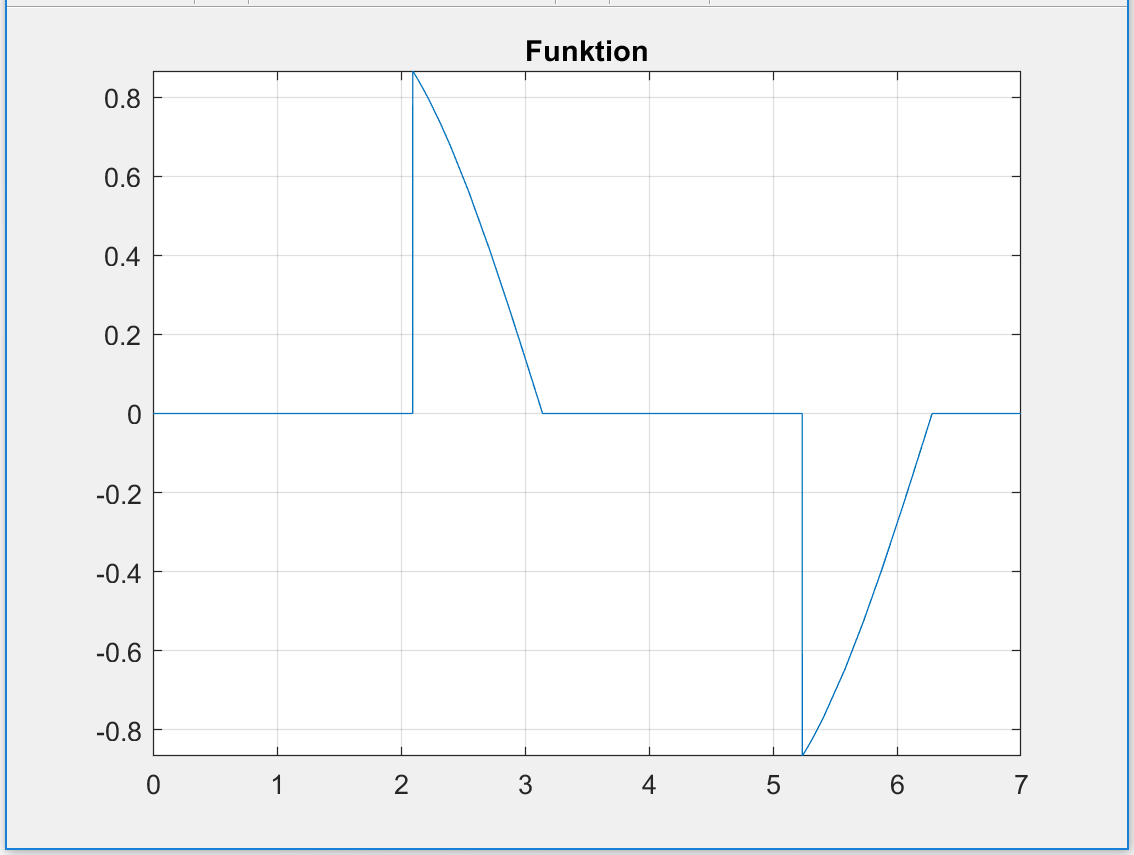
\includegraphics[width=0.4\linewidth]{eingangssignal_120.png}\label{fig:eingangssignal_120}}\qquad
	\subfloat[][]{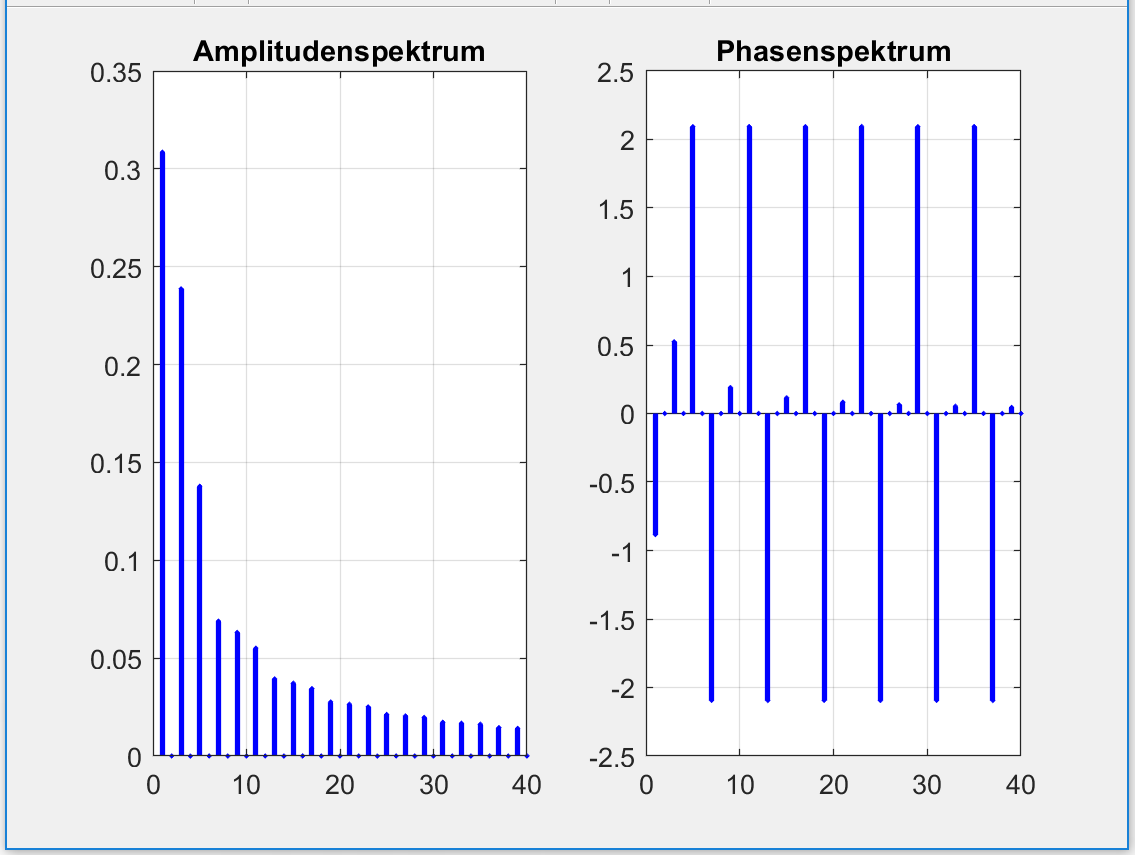
\includegraphics[width=0.4\linewidth]{A_PH_120.png}\label{fig:A_PH_120}}
	\caption{Phasenanschnittsteuerung mit 120\textdegree (a) Eingangssignal (b) Amplituden- und Phasenspektrum}
	\label{fig:Phasenanschnittsteuerung_mit_120}
\end{figure}

\newpage

\begin{figure}[ht!]
	\centering
	\subfloat[][]{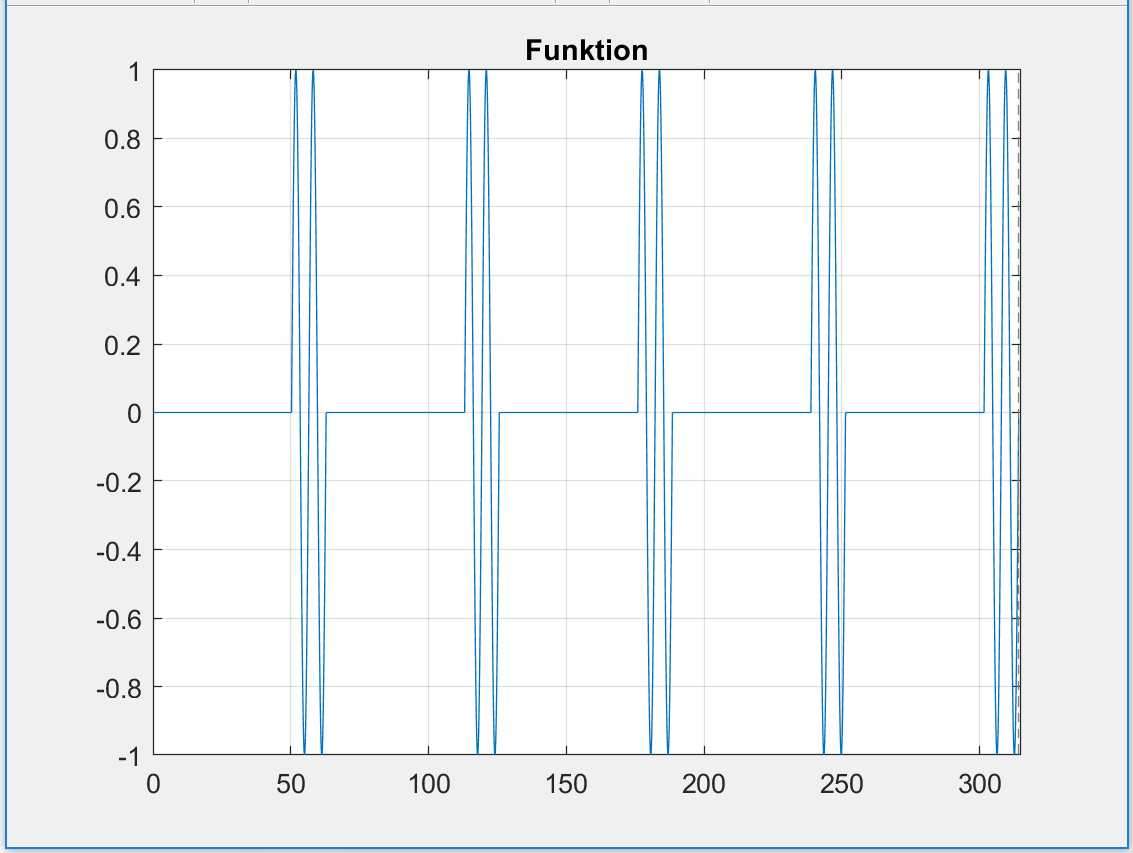
\includegraphics[width=0.4\linewidth]{Schwingungspaket_0_2.png}\label{fig:Schwingungspaket_0_2}}\qquad
	\subfloat[][]{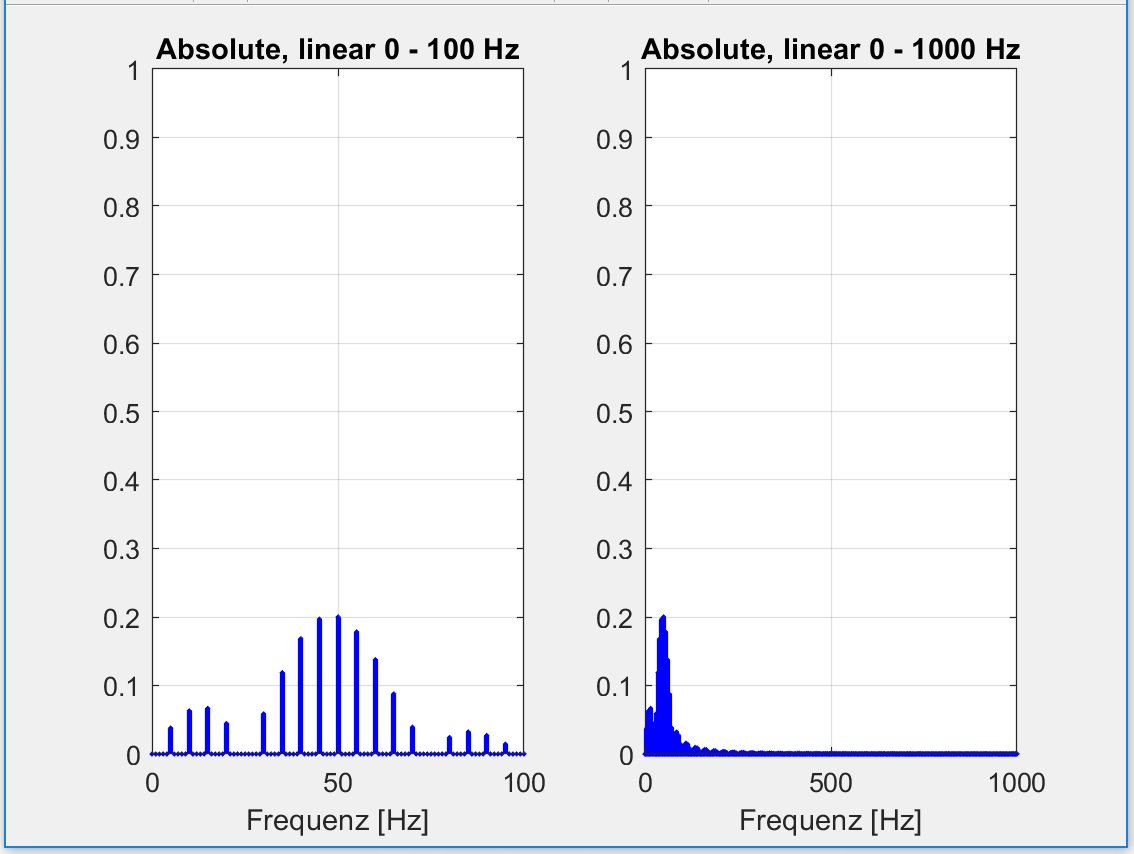
\includegraphics[width=0.4\linewidth]{Oberwellen_0_2.png}\label{fig:Oberwellen_0_2}}
	\caption{Schwingungspaket mit duty cycle 0.2 (a) Eingangssignal (b) Amplituden- und Phasenspektrum}
	\label{fig:Schwingungspaketsteuerung_mit_duty_cycle_0_2}
\end{figure}


\begin{figure}[ht!]
	\centering
	\subfloat[][]{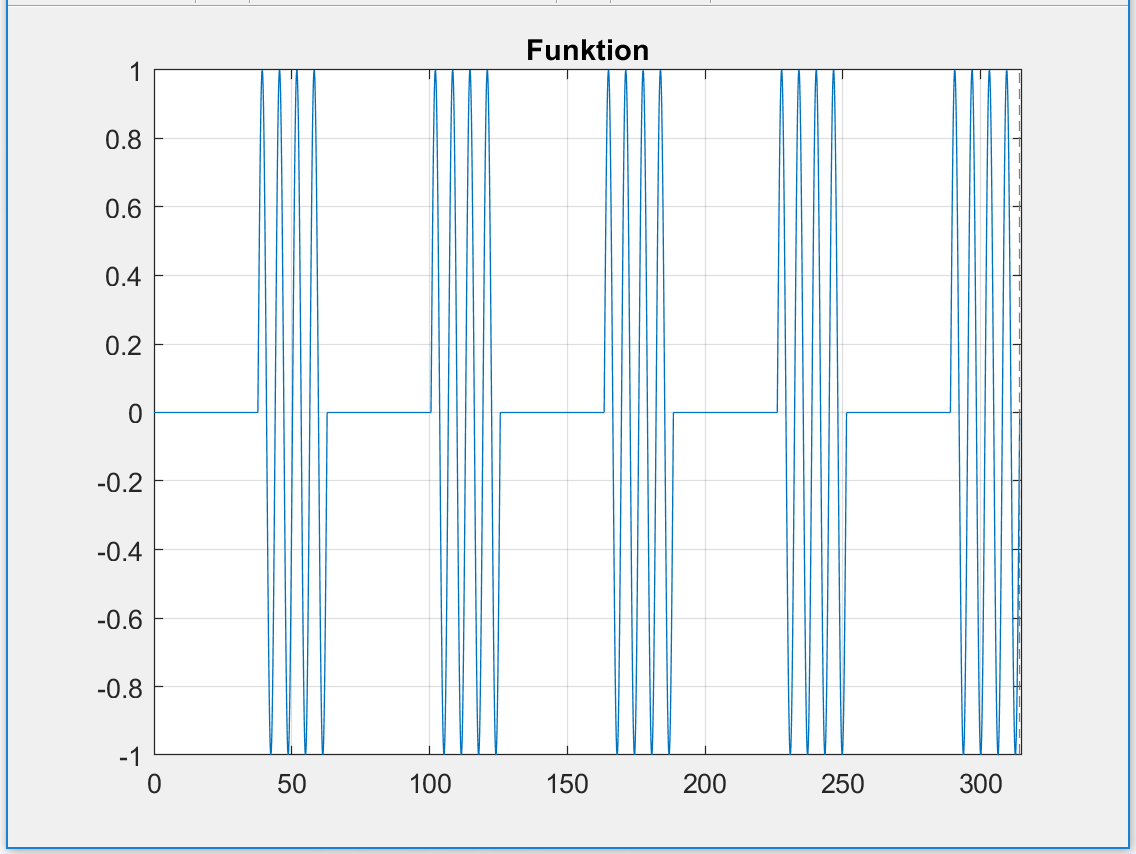
\includegraphics[width=0.4\linewidth]{Schwingungspaket_0_4.png}\label{fig:Schwingungspaket_0_4}}\qquad
	\subfloat[][]{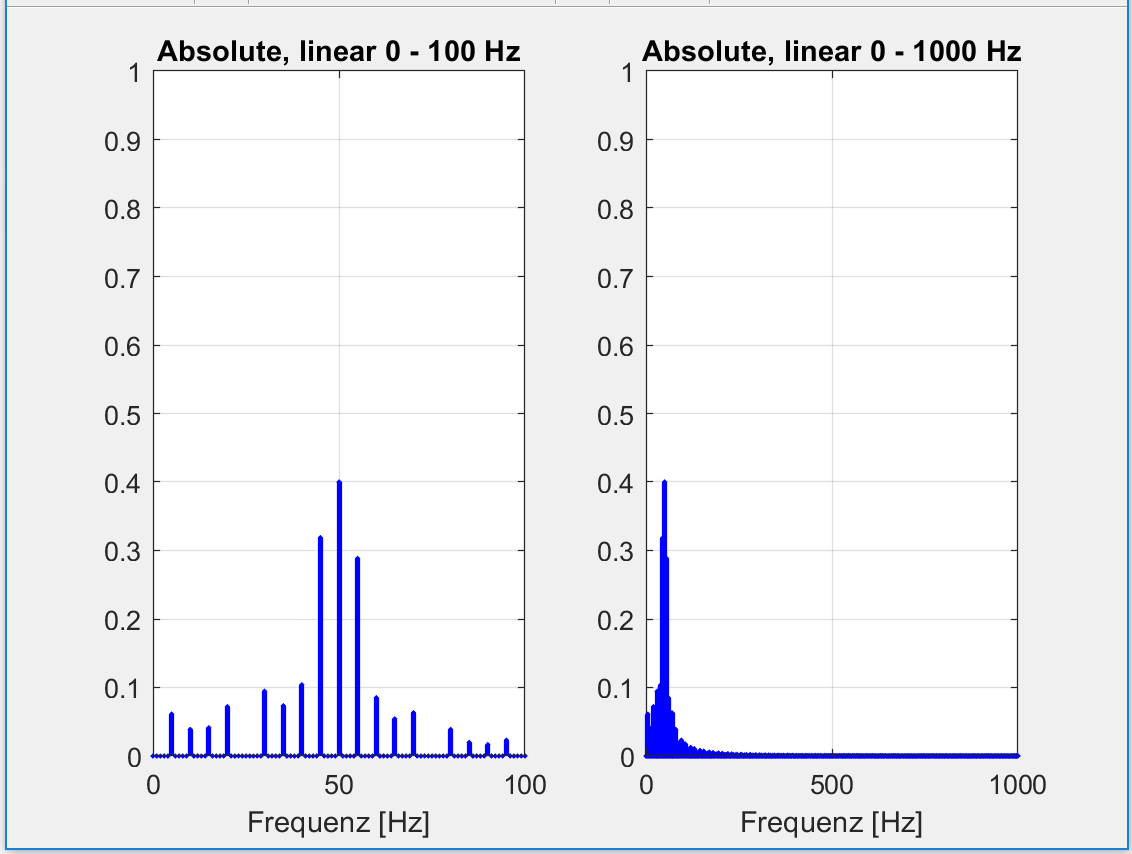
\includegraphics[width=0.4\linewidth]{Oberwellen_0_4.png}\label{fig:Oberwellen_0_4}}
	\caption{Schwingungspaket mit duty cycle 0.4 (a) Eingangssignal (b) Amplituden- und Phasenspektrum}
	\label{fig:Schwingungspaketsteuerung_mit_duty_cycle_0_4}
\end{figure}

\begin{figure}[ht!]
	\centering
	\subfloat[][]{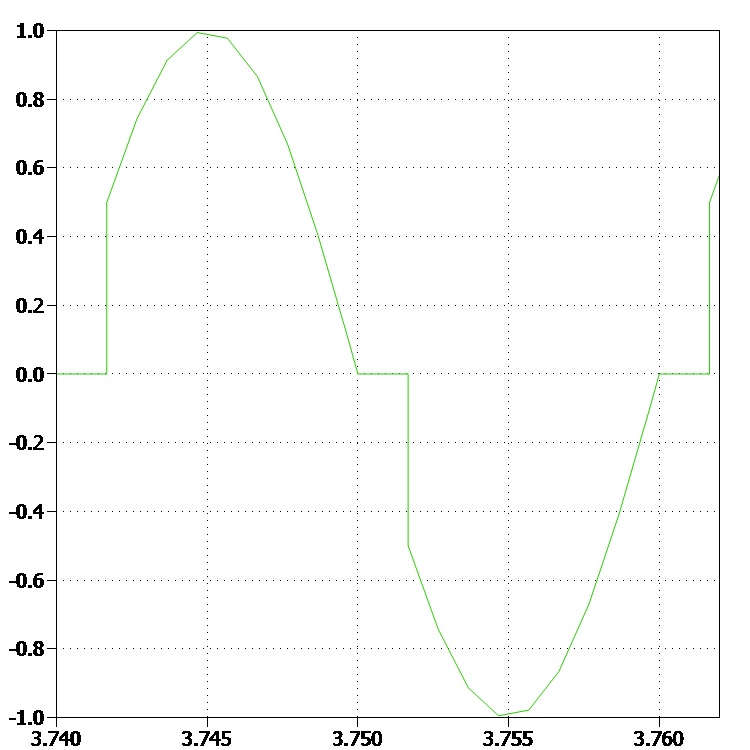
\includegraphics[width=0.32\linewidth]{plecs_phasenanschnitt_pi_6_funktion.png}\label{fig:plecs_phasenanschnitt_pi_6_funktion}}\qquad
	\subfloat[][]{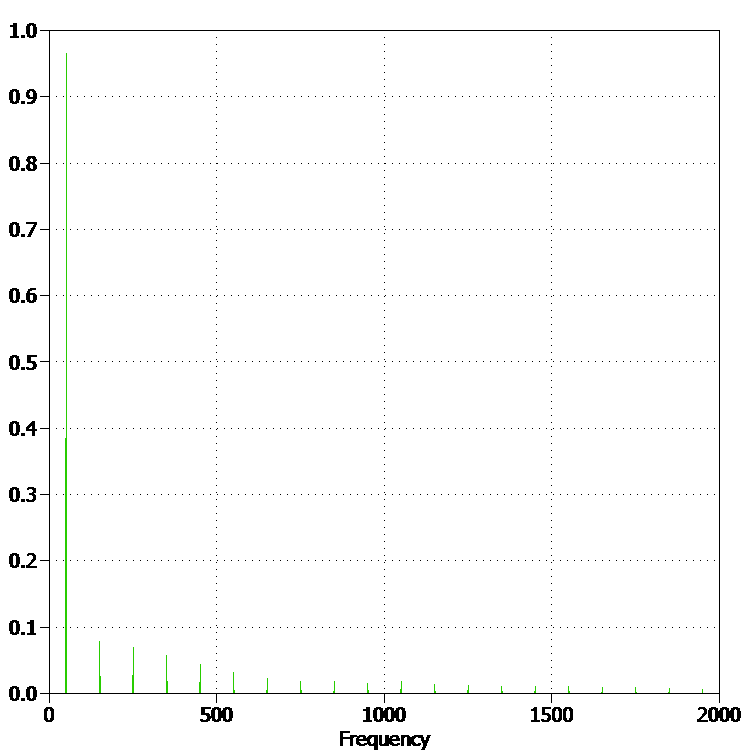
\includegraphics[width=0.32\linewidth]{plecs_phasenanschnitt_pi_6.png}\label{fig:plecs_phasenanschnitt_pi_6}}
	\caption{Phasenanschnitt mit 30\textdegree simuliert mit Plecs (a) Eingangssignal (b) Amplituden- und Phasenspektrum}
	\label{fig:Plecs_mit_phasenanschnitt_30}
\end{figure}

\newpage

\begin{figure}[ht!]
	\centering
	\subfloat[][]{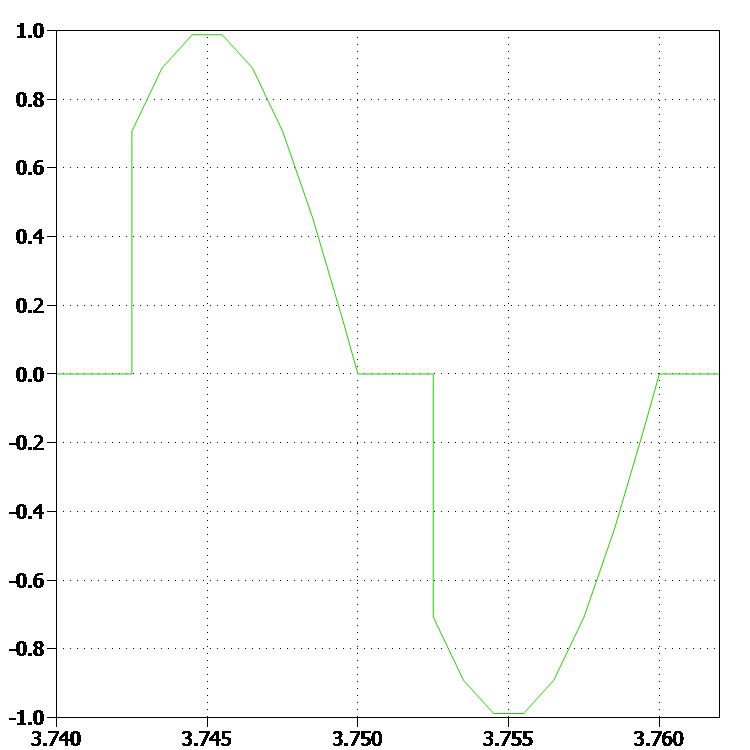
\includegraphics[width=0.32\linewidth]{plecs_phasenanschnitt_pi_4_funktion.png}\label{fig:plecs_phasenanschnitt_pi_4_funktion}}\qquad
	\subfloat[][]{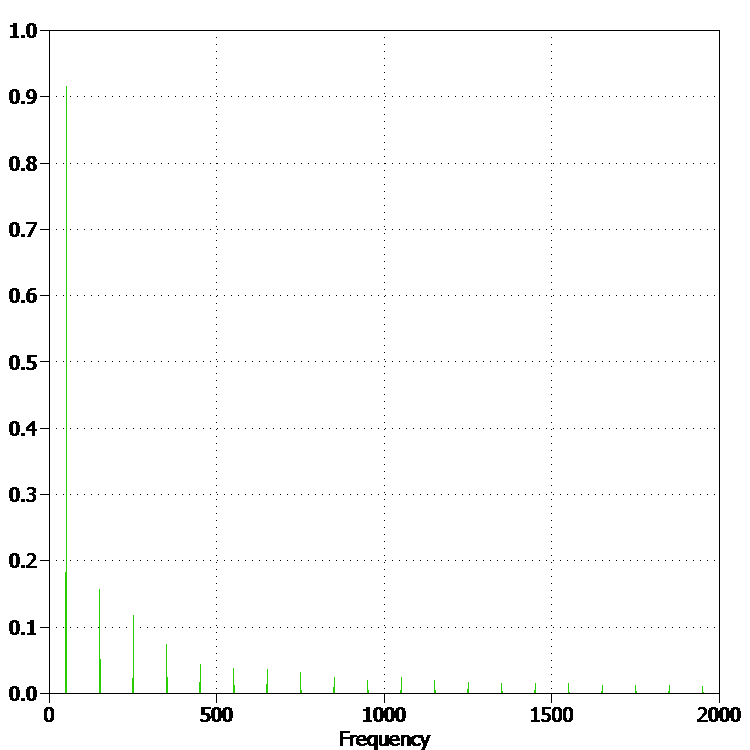
\includegraphics[width=0.32\linewidth]{plecs_phasenanschnitt_pi_4.png}\label{fig:plecs_phasenanschnitt_pi_4}}
	\caption{Phasenanschnitt mit 45\textdegree simuliert mit Plecs (a) Eingangssignal (b) Amplituden- und Phasenspektrum}
	\label{fig:Plecs_mit_phasenanschnitt_45}
\end{figure}


\begin{figure}[ht!]
	\centering
	\subfloat[][]{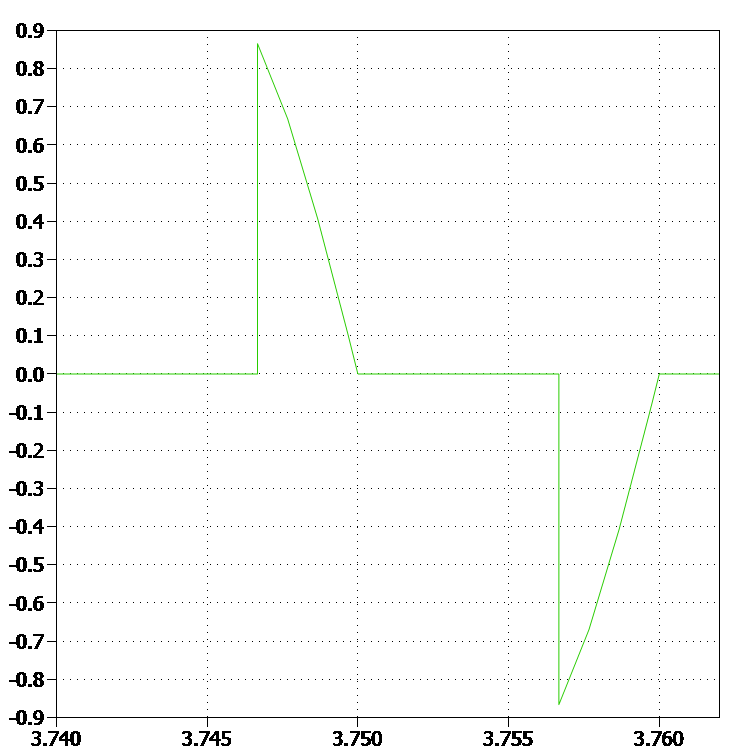
\includegraphics[width=0.32\linewidth]{plecs_phasenanschnitt_120_funktion.png}\label{fig:plecs_phasenanschnitt_120_funktion}}\qquad
	\subfloat[][]{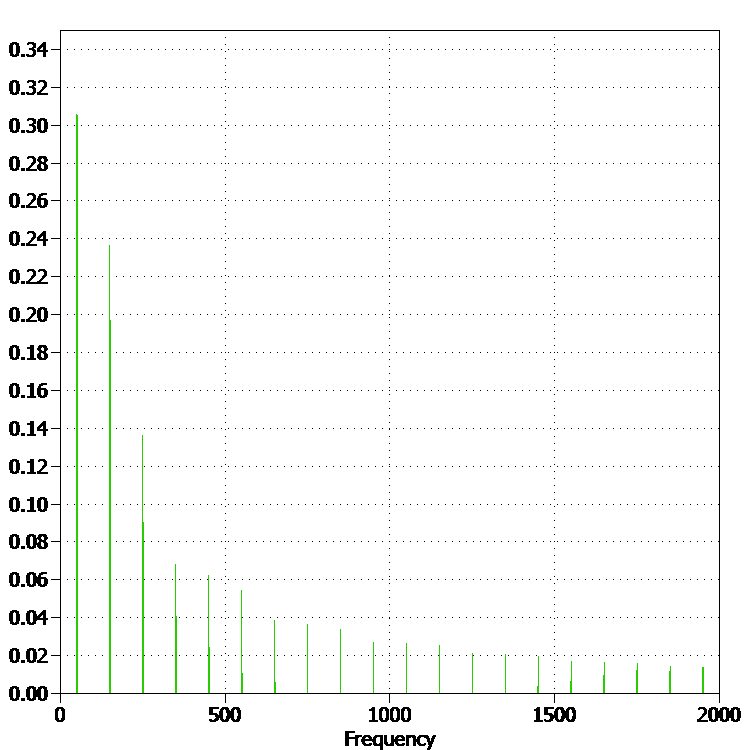
\includegraphics[width=0.32\linewidth]{plecs_phasenanschnitt_120.png}\label{fig:plecs_phasenanschnitt_120}}
	\caption{Phasenanschnitt mit 120\textdegree simuliert mit Plecs (a) Eingangssignal (b) Amplituden- und Phasenspektrum}
	\label{fig:Plecs_mit_phasenanschnitt_120}
\end{figure}


\begin{figure}[ht!]
	\centering
	\subfloat[][]{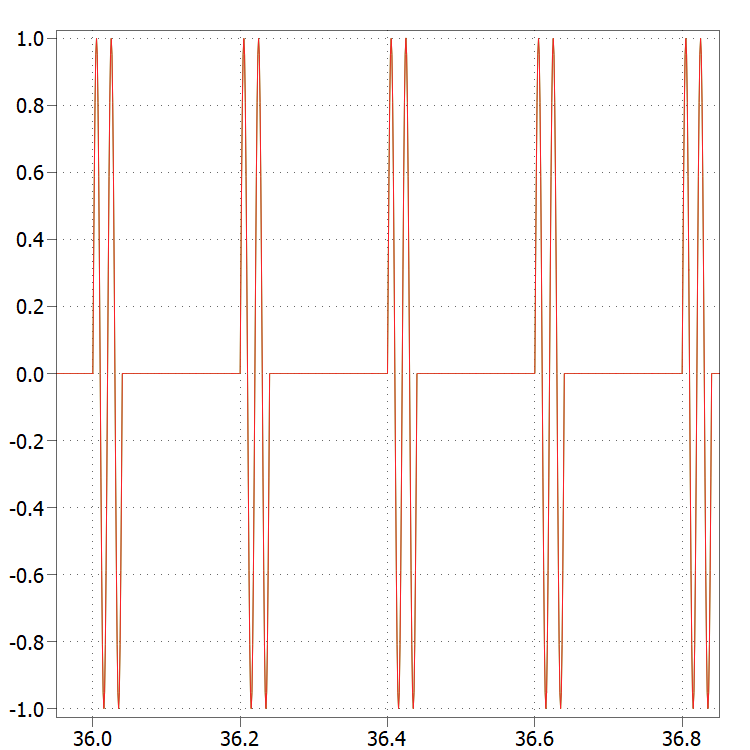
\includegraphics[width=0.32\linewidth]{plecs_schwingungspacket_0_2_schwingungen.PNG}\label{fig:plecs_schwingungspacket_0_2_schwingungen}}\qquad
	\subfloat[][]{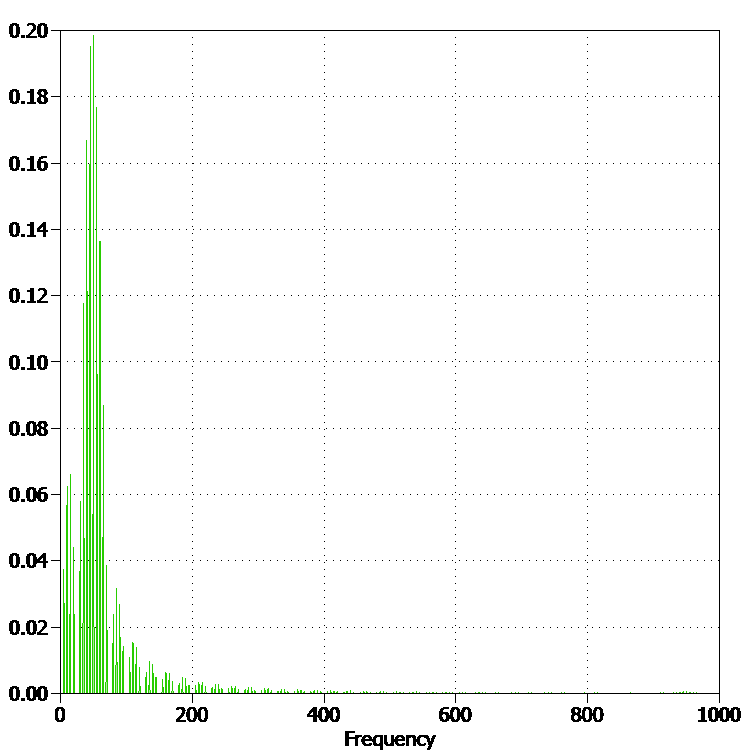
\includegraphics[width=0.32\linewidth]{plecs_schwingungspacket_0_2_1000.PNG}\label{fig:plecs_schwingungspacket_0_2_1000}}
	\caption{Schwingungspaketsteuerung mit duty cycle 0.2 simuliert mit Plecs (a) Eingangssignal (b) Amplitudenspektrum}
	\label{fig:Schwingungspaketsteuerung_mit_duty_cycle_0_2 simuliert_mit_Plecs}
\end{figure}

\newpage

\begin{figure}[ht!]
	\centering
	\subfloat[][]{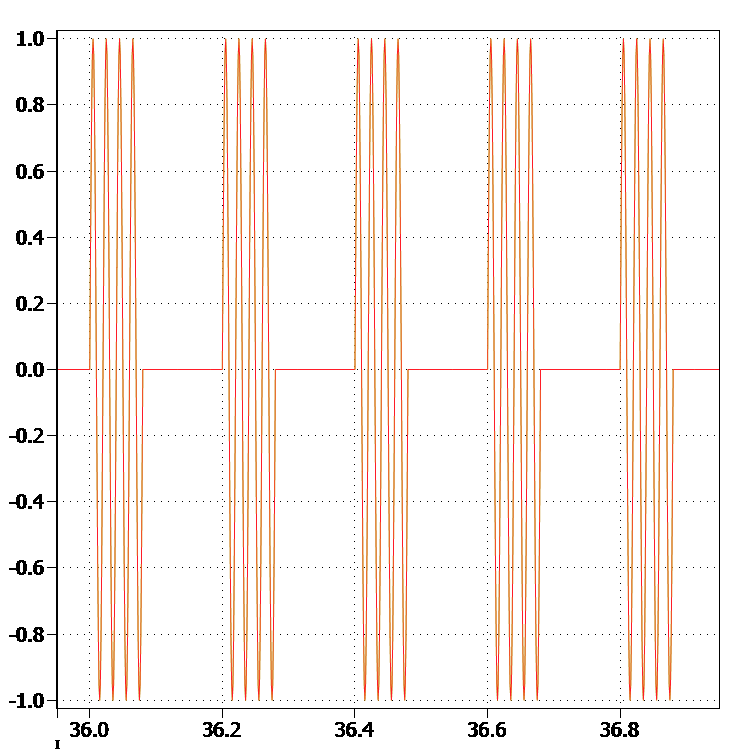
\includegraphics[width=0.32\linewidth]{plecs_schwingungspacket_0_4_schwingungen.PNG}\label{fig:plecs_schwingungspacket_0_4_schwingungen}}\qquad
	\subfloat[][]{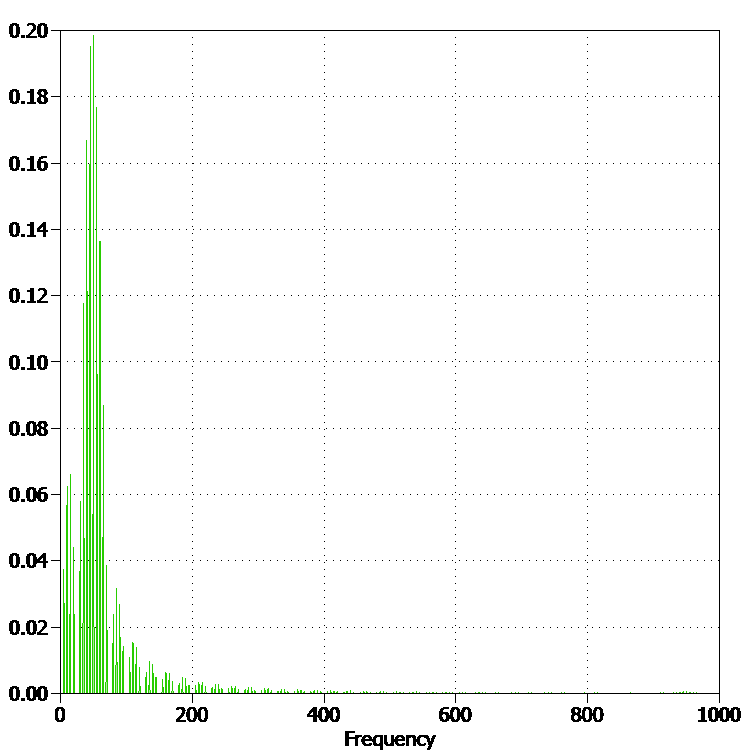
\includegraphics[width=0.32\linewidth]{plecs_schwingungspacket_0_2_1000.PNG}\label{fig:plecs_schwingungspacket_0_4_1000}}
	\caption{Schwingungspaketsteuerung mit duty cycle 0.4 simuliert mit Plecs (a) Eingangssignal (b) Amplitudenspektrum}
	\label{fig:Schwingungspaketsteuerung_mit_duty_cycle_0_4 simuliert_mit_Plecs}
\end{figure}


\begin{figure}[ht!]
	\centering
	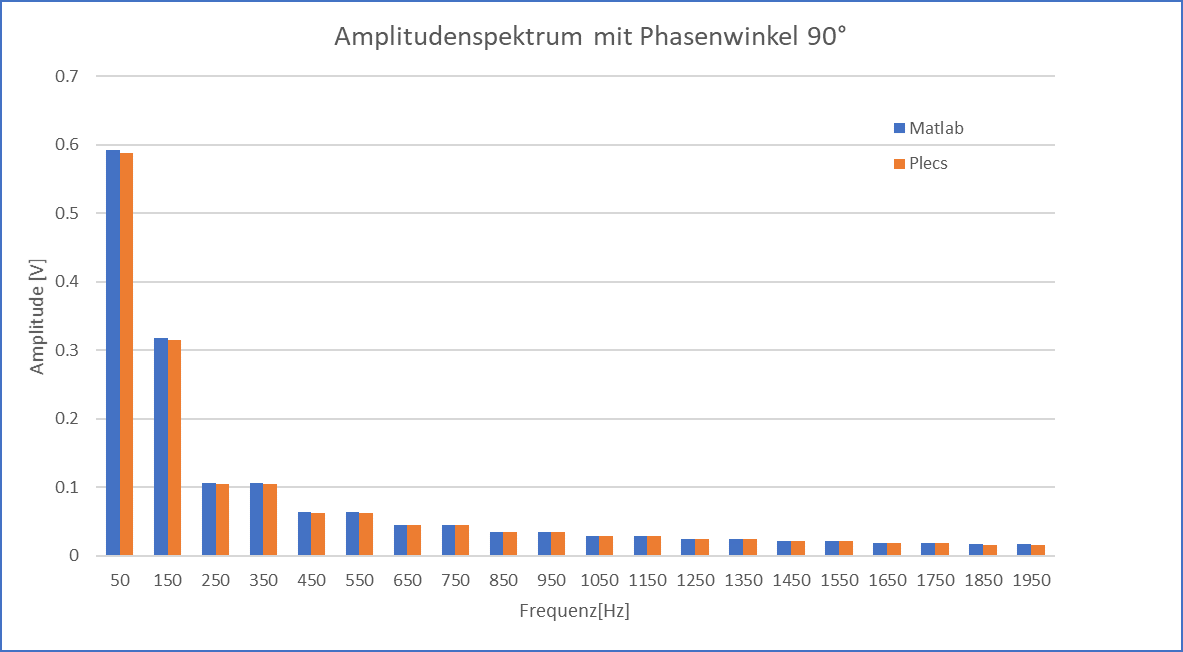
\includegraphics[scale=0.55]{Vergleich_Amplitudenspektrum_mit_Phasenwinkel_90.png}	
	\caption{Vergleich der Amplitudenspektrum mit Phasenwinkel von 90\textdegree}
	\label{fig:Vergleich_der_Amplitudenspektrum_mit Phasenwinkel_von_90}
\end{figure}

\begin{figure}[ht!]
	\centering
	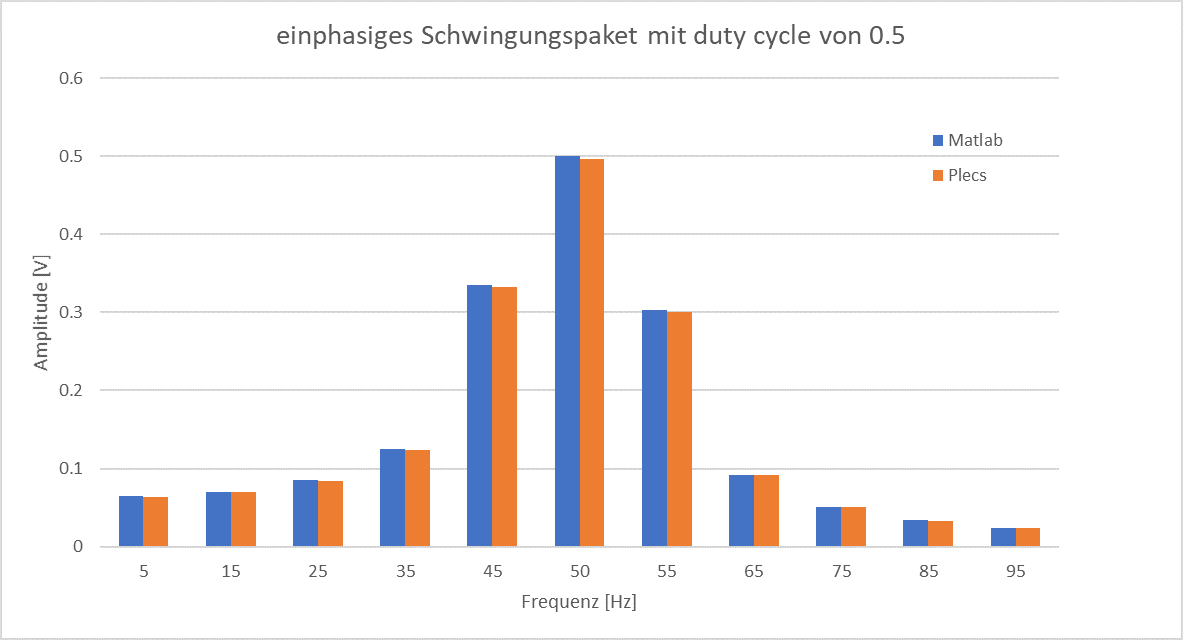
\includegraphics[scale=0.55]{Vergleich_einphasiges_Schwingungspaket_mit_duty_cycle_von_0_5.png}	
	\caption{Vergleich des Schwingungspaket mit duty cycle von 0.5}
	\label{fig:Vergleich des Schwingungspaket mit duty cycle von 0.5}
\end{figure}

\newpage

\begin{figure}[ht!]
	\centering
	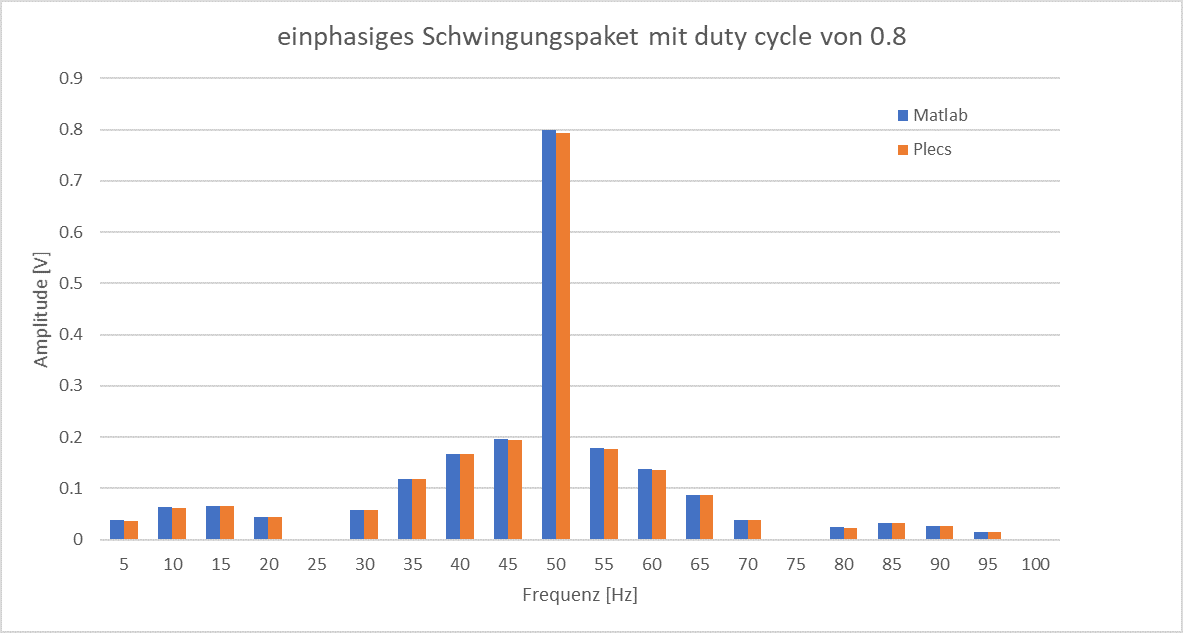
\includegraphics[scale=0.55]{Vergleich_einphasiges_Schwingungspaket_mit_duty_cycle_von_0_8.png}	
	\caption{Vergleich des Schwingungspaket mit duty cycle von 0.8}
	\label{fig:Vergleich des Schwingungspaket mit duty cycle von 0.8}
\end{figure}

\begin{figure}[ht!]
	\centering
	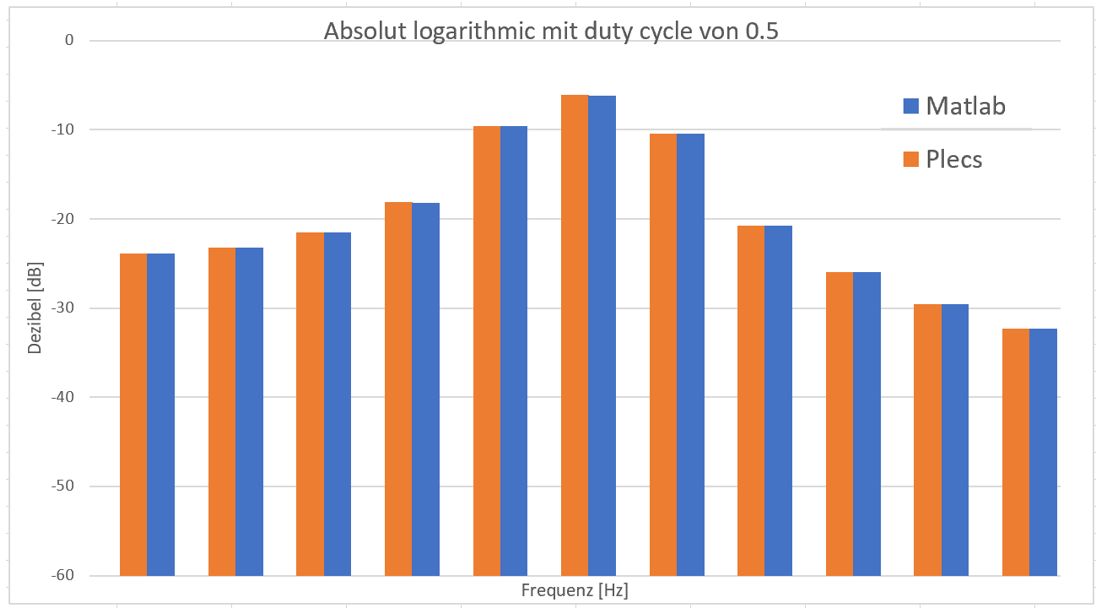
\includegraphics[scale=0.55]{Vergleich_absolut_logarithmic_duty_cycle_von_0_5_mit_legende.PNG}	
	\caption{Vergleich des Schwingungspaket mit duty cycle von 0.8}
	\label{fig:Vergleich_absolut_logarithmic_duty_cycle_von_0_5_mit_legende}
\end{figure}

\begin{figure}[ht!]
	\centering
	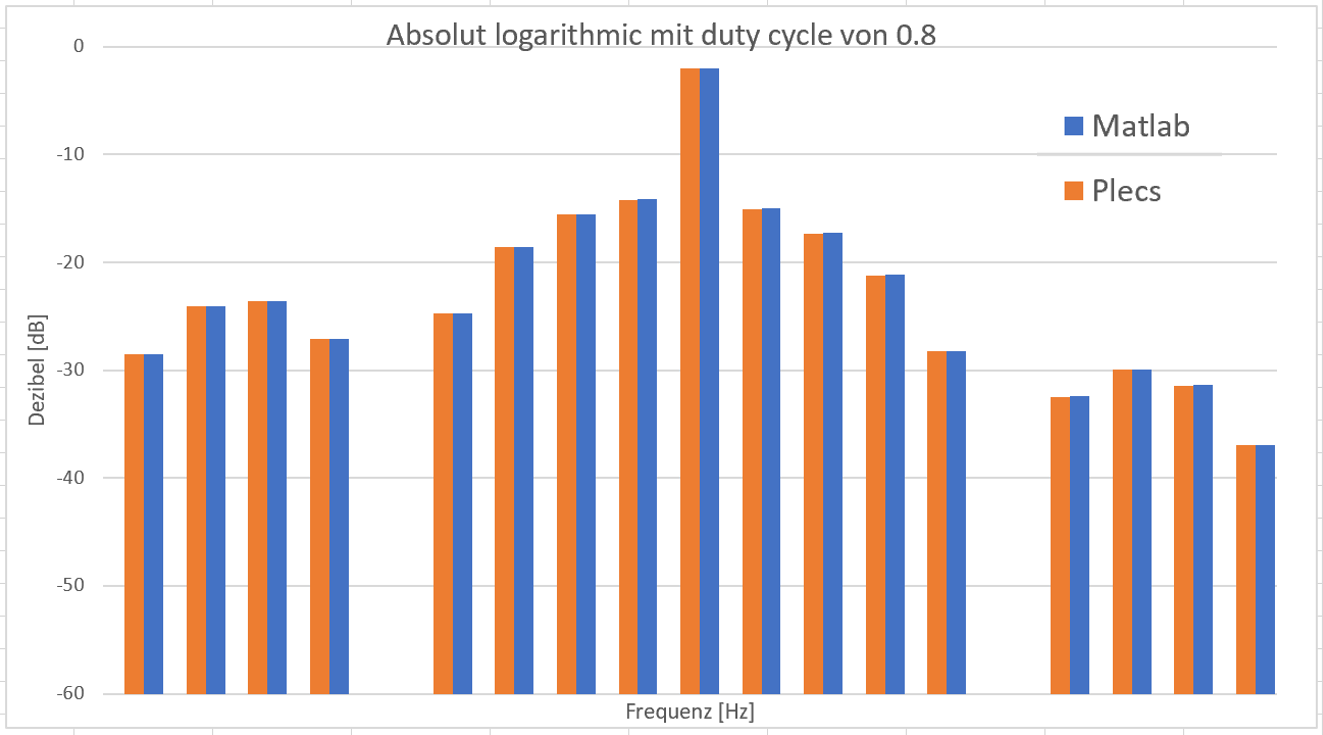
\includegraphics[scale=0.55]{Vergleich_absolut_logarithmic_duty_cycle_von_0_8_mit_legende.PNG}	
	\caption{Vergleich des Schwingungspaket mit duty cycle von 0.8}
	\label{fig:Vergleich_absolut_logarithmic_duty_cycle_von_0_8_mit_legende}
\end{figure}

\subsection{Messungen Spannungen Widerstand}\label{sec:Mess_Spannung_Widerstand}
\subsubsection*{Phasenanschnitt 60\textdegree}

\begin{figure}[ht!]
	\centering
	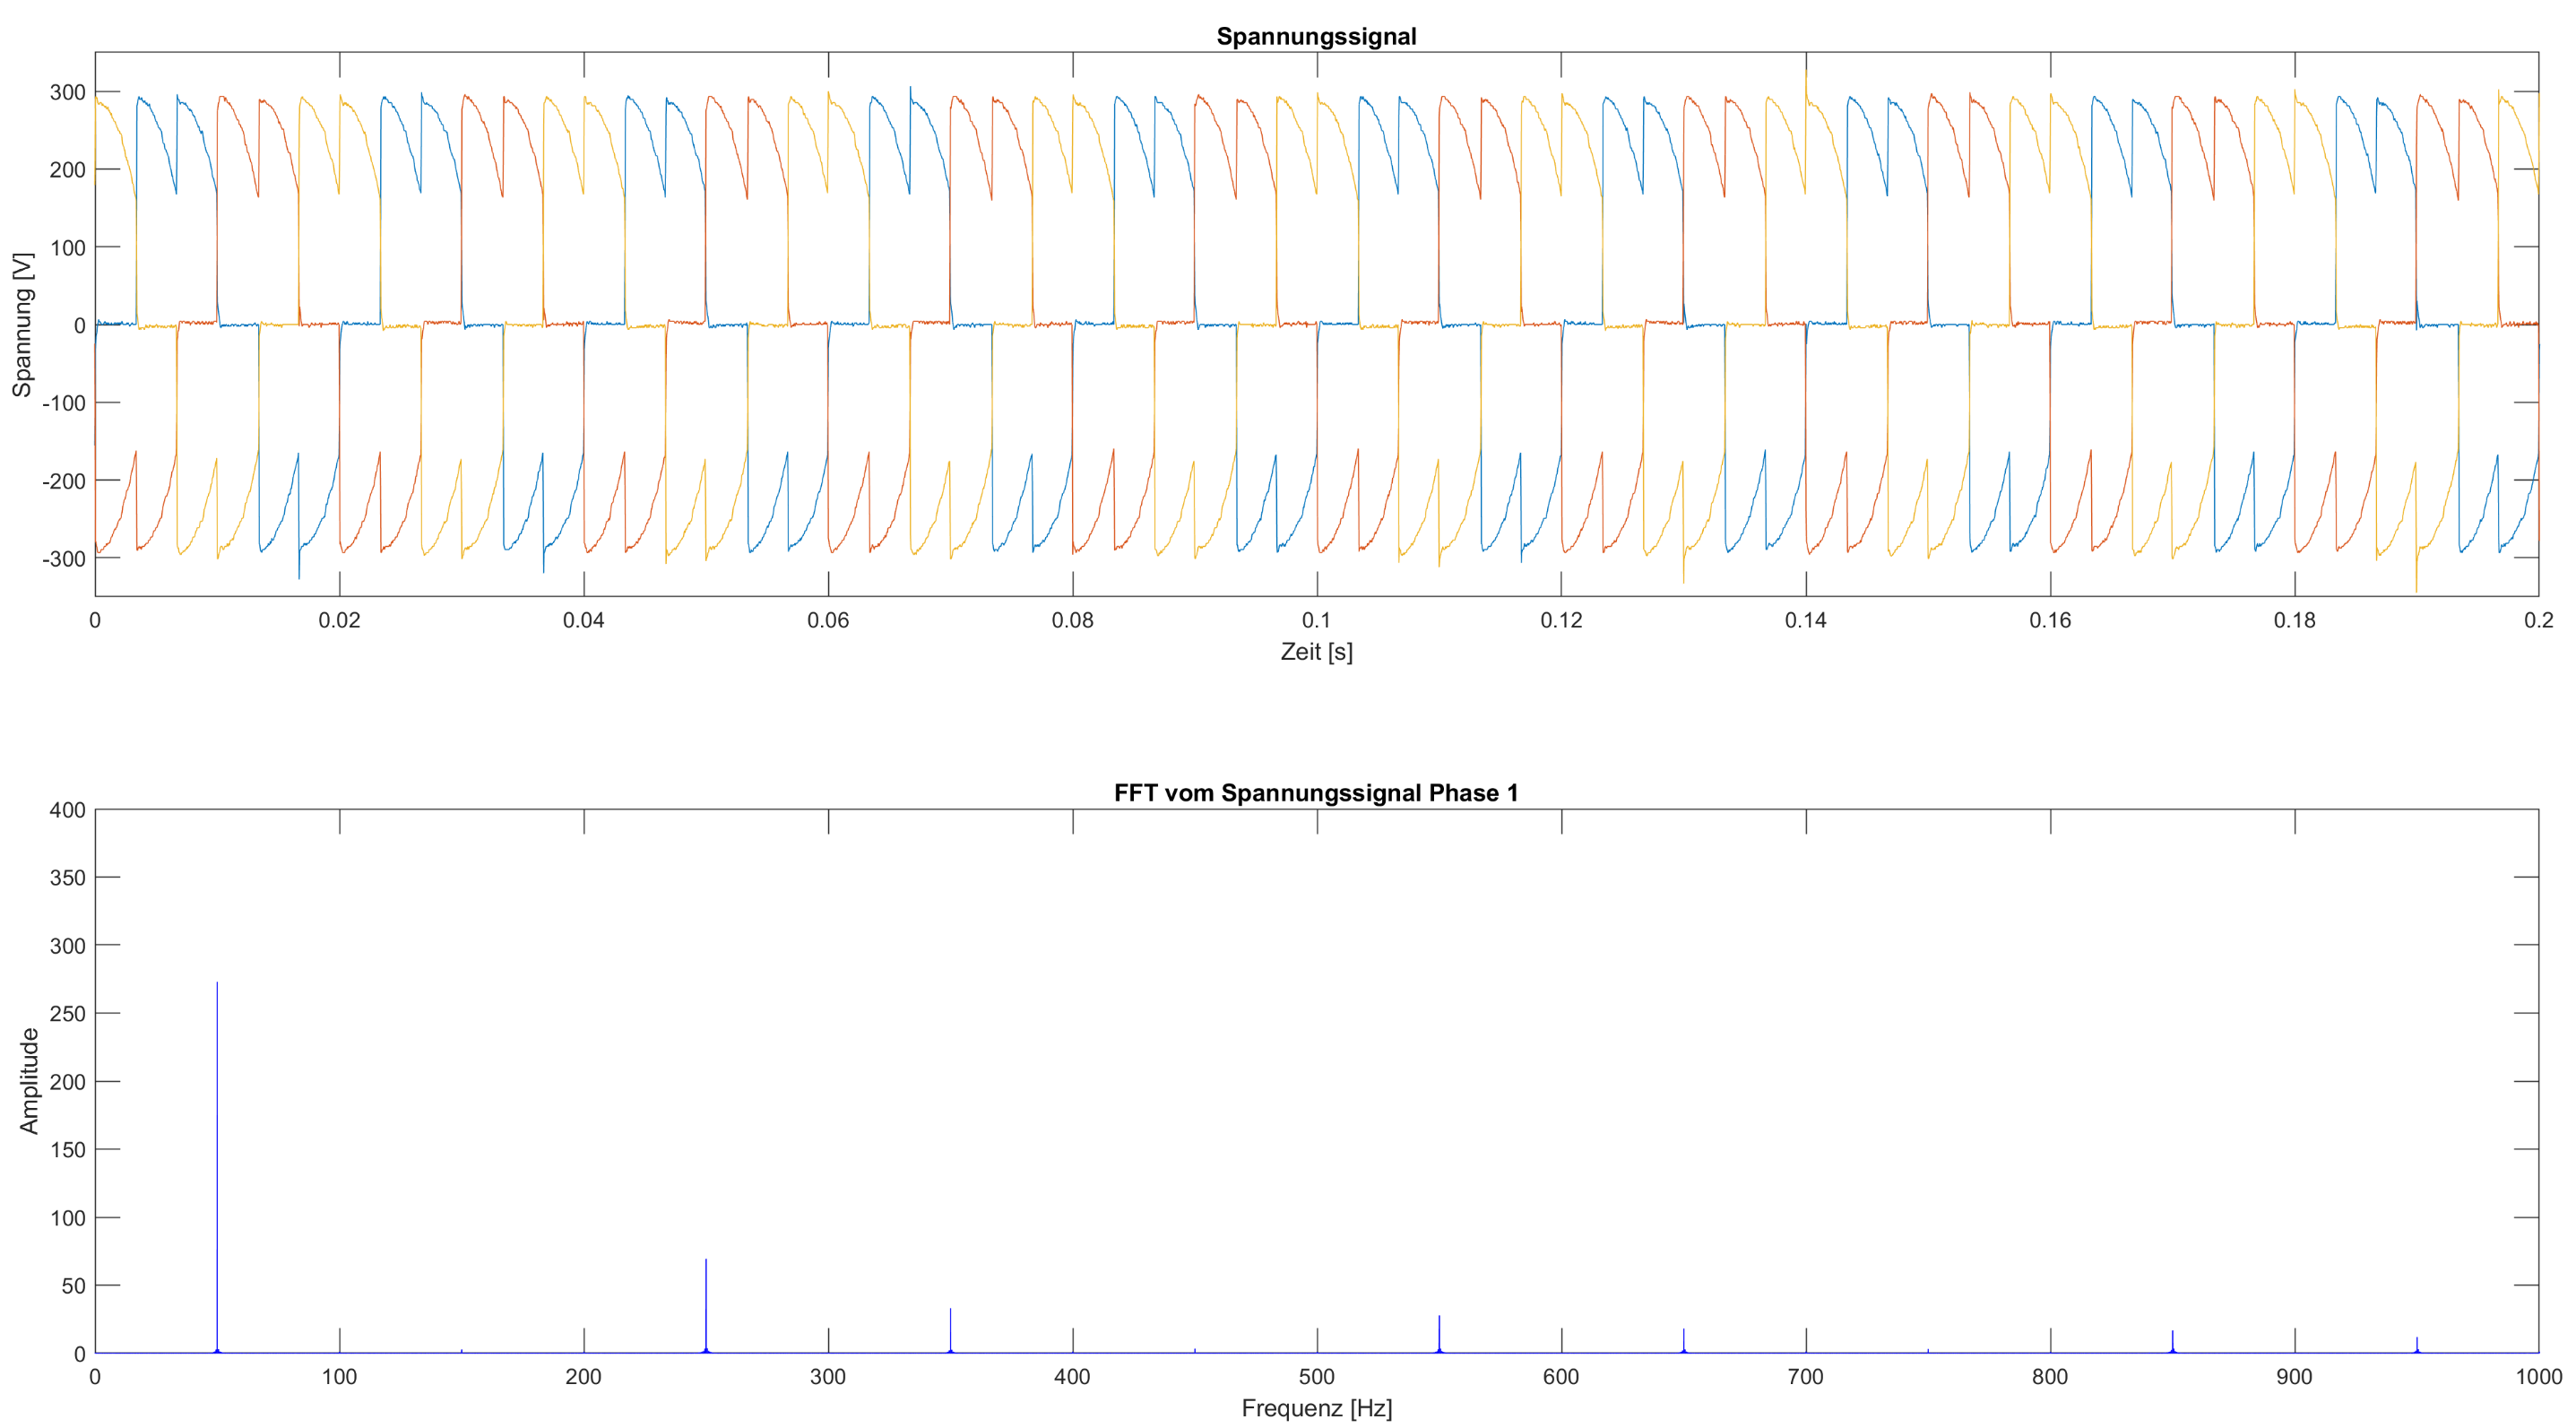
\includegraphics[width=\textwidth]{Messung_Widerstand_Phas_60grad.png}	
	\caption{Messung mit Phasenanschnitt 60\textdegree}\label{fig:Mess_Phas_60}
\end{figure}
\newpage
\subsubsection*{Phasenanschnitt 90\textdegree}
\begin{figure}[ht!]
	\centering
	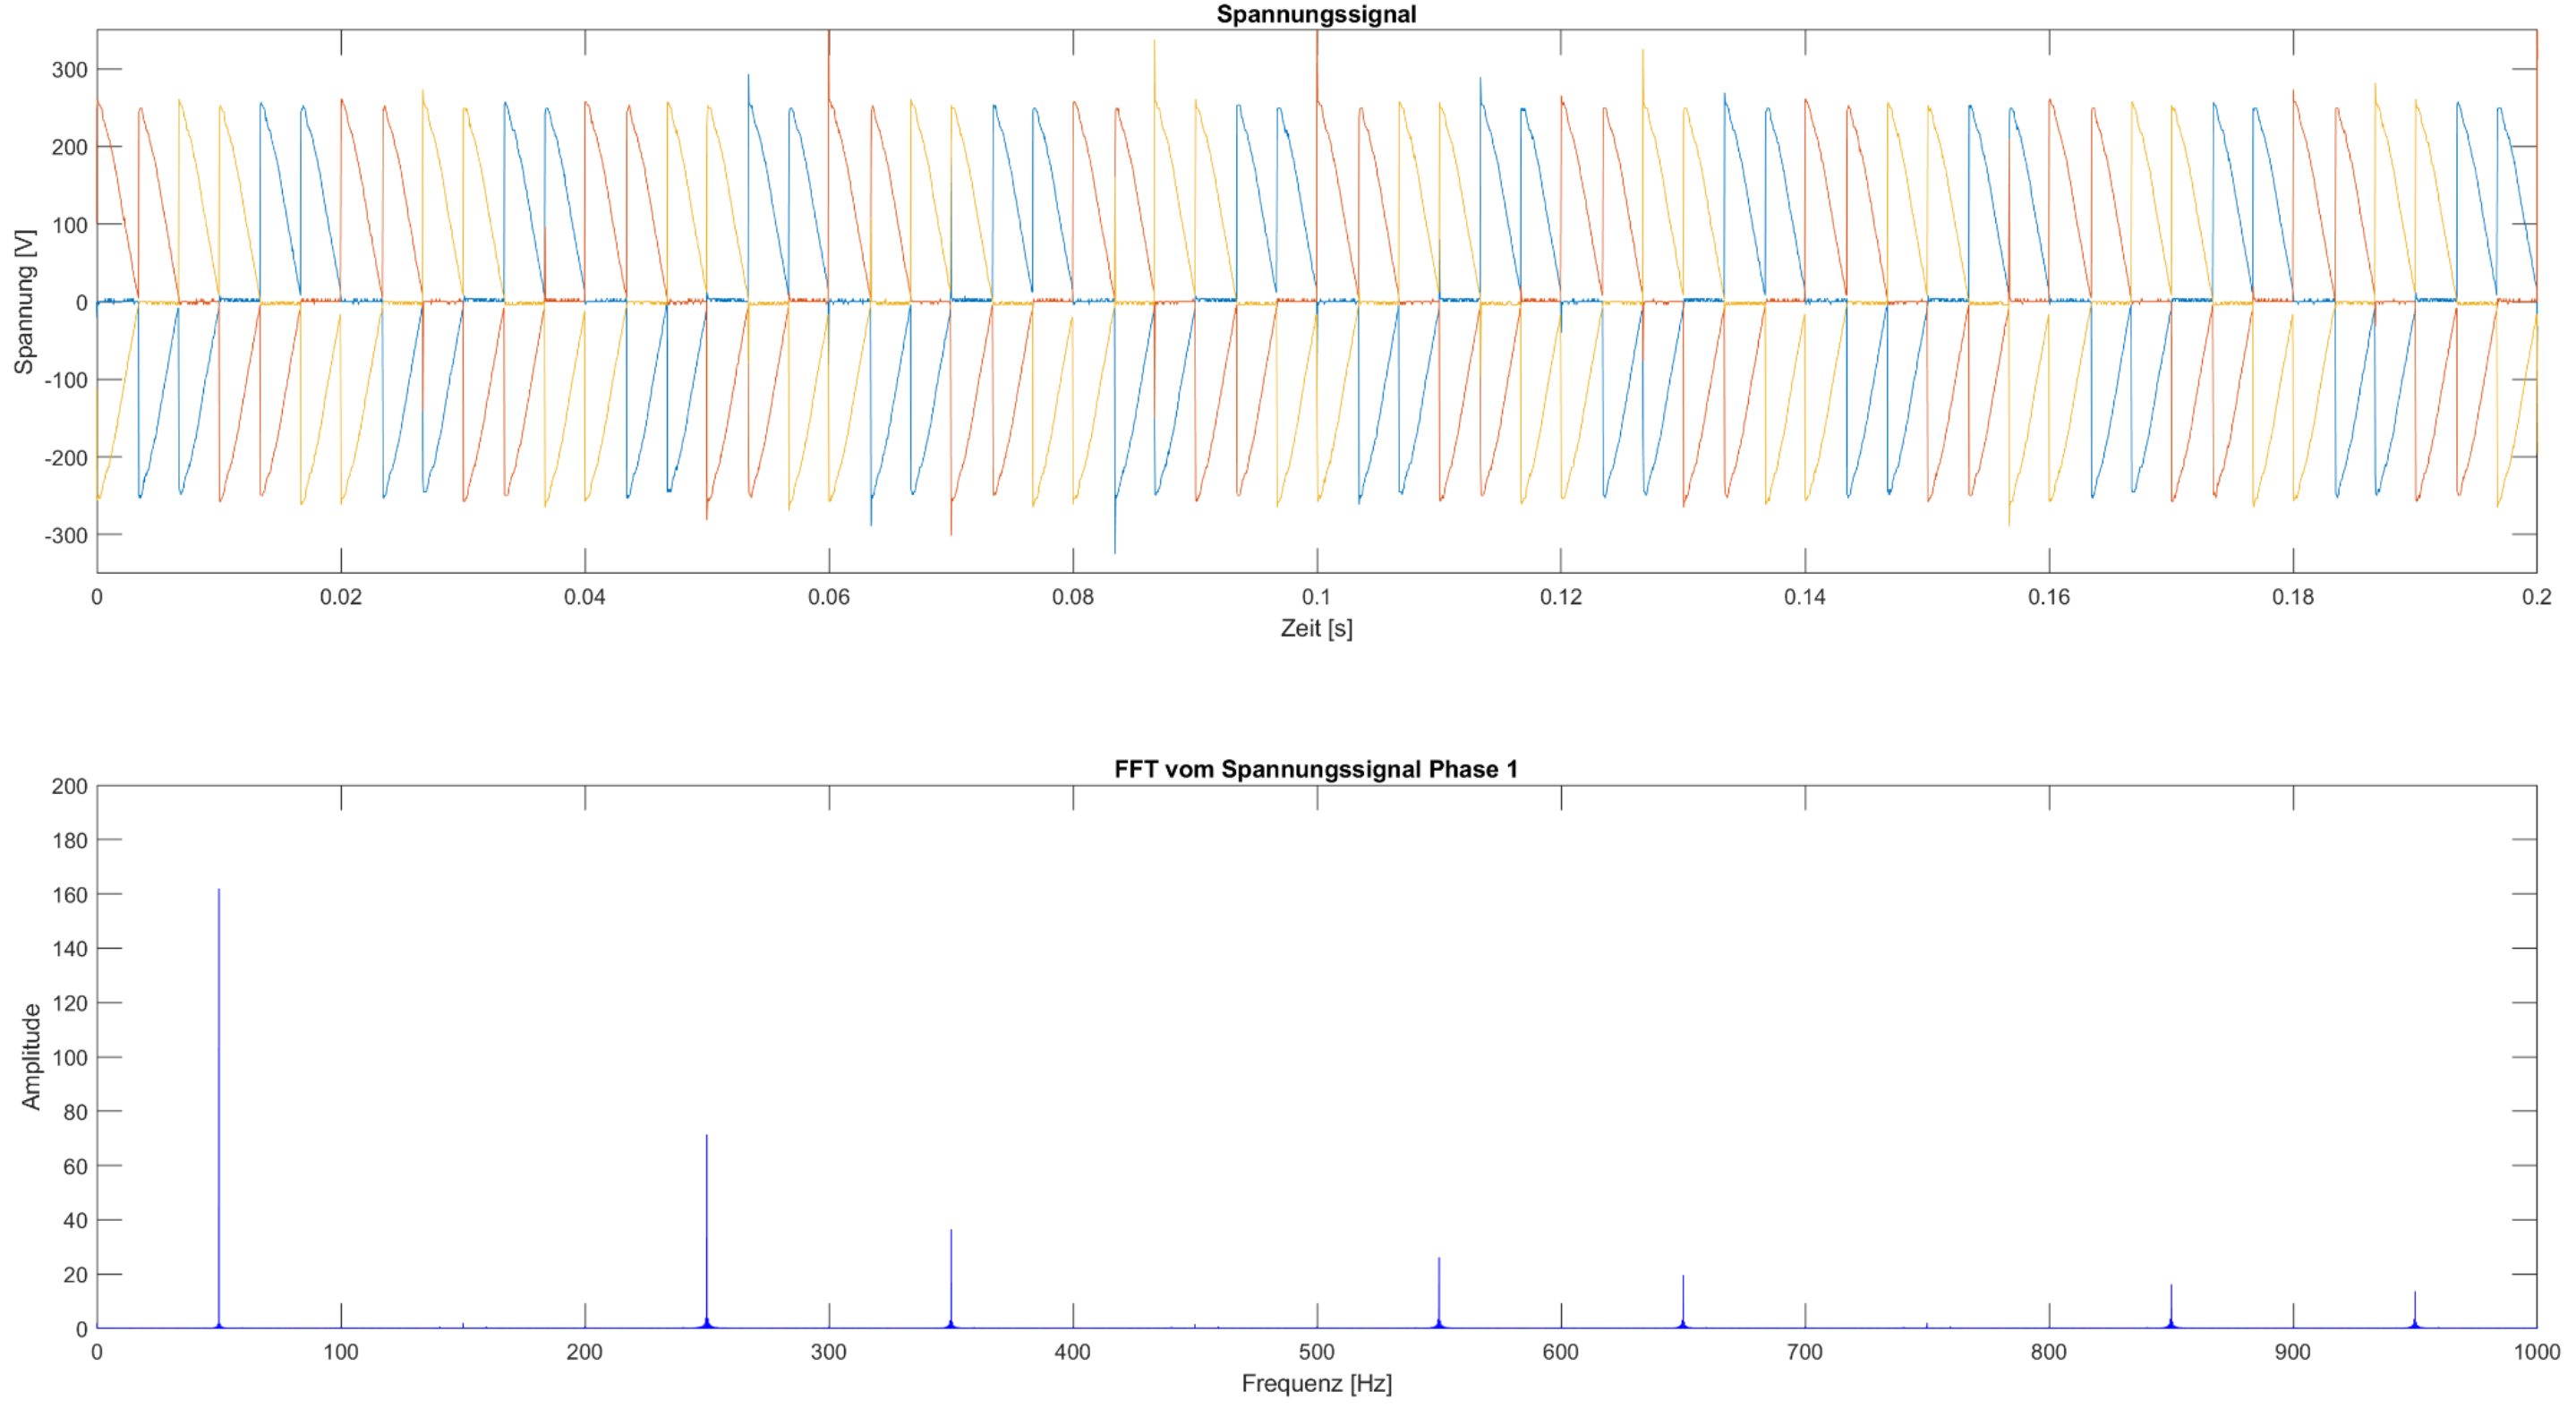
\includegraphics[width=\textwidth]{Messung_Widerstand_Phas_90grad.png}	
	\caption{Messung mit Phasenanschnitt 90\textdegree}\label{fig:Mess_Phas_90}
\end{figure}

\subsection{Messungen Spannungen ASM}\label{sec:Mess_Spannung_ASM}
\subsubsection*{Schwingungspaket 50\%}
\begin{figure}[ht!]
	\centering
	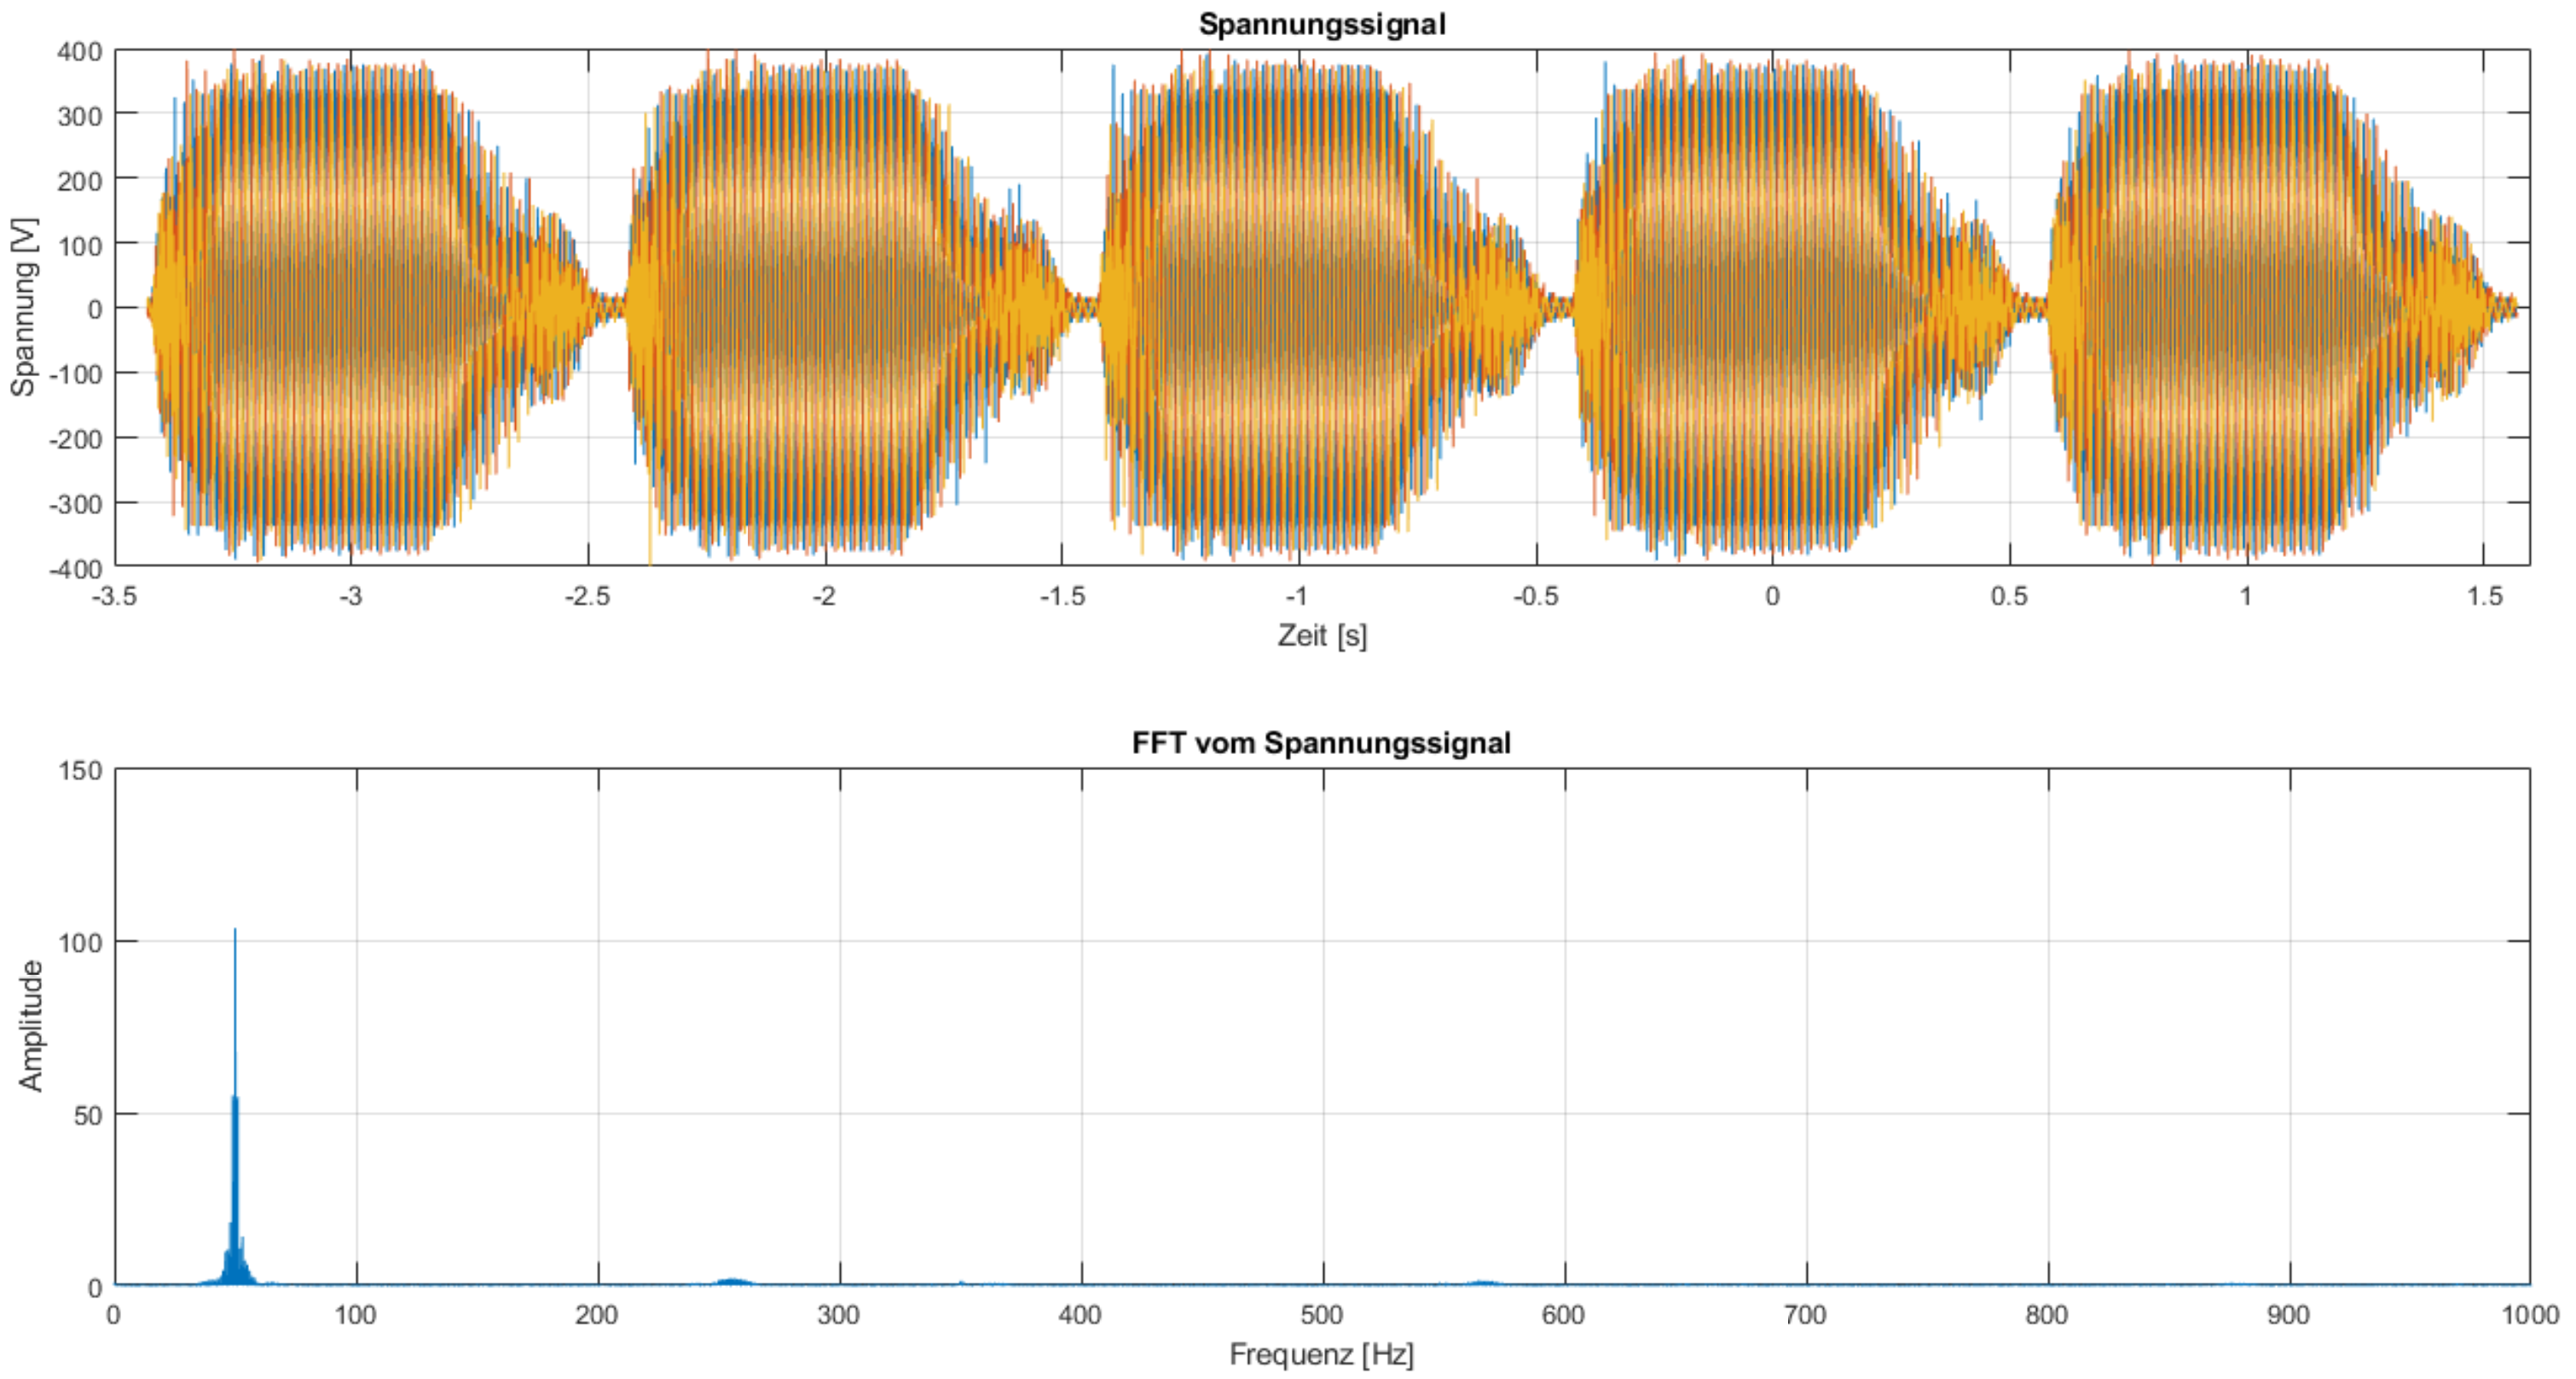
\includegraphics[width=\textwidth]{Messung_ASM_Schwing_0_5.png}	
	\caption{Messung mit Schwingungspaket 50\%}\label{fig:Mess_ASM_Schwing_0_5}
\end{figure}

\newpage
\subsubsection*{Schwingungspaket 80\%}
\begin{figure}[ht!]
	\centering
	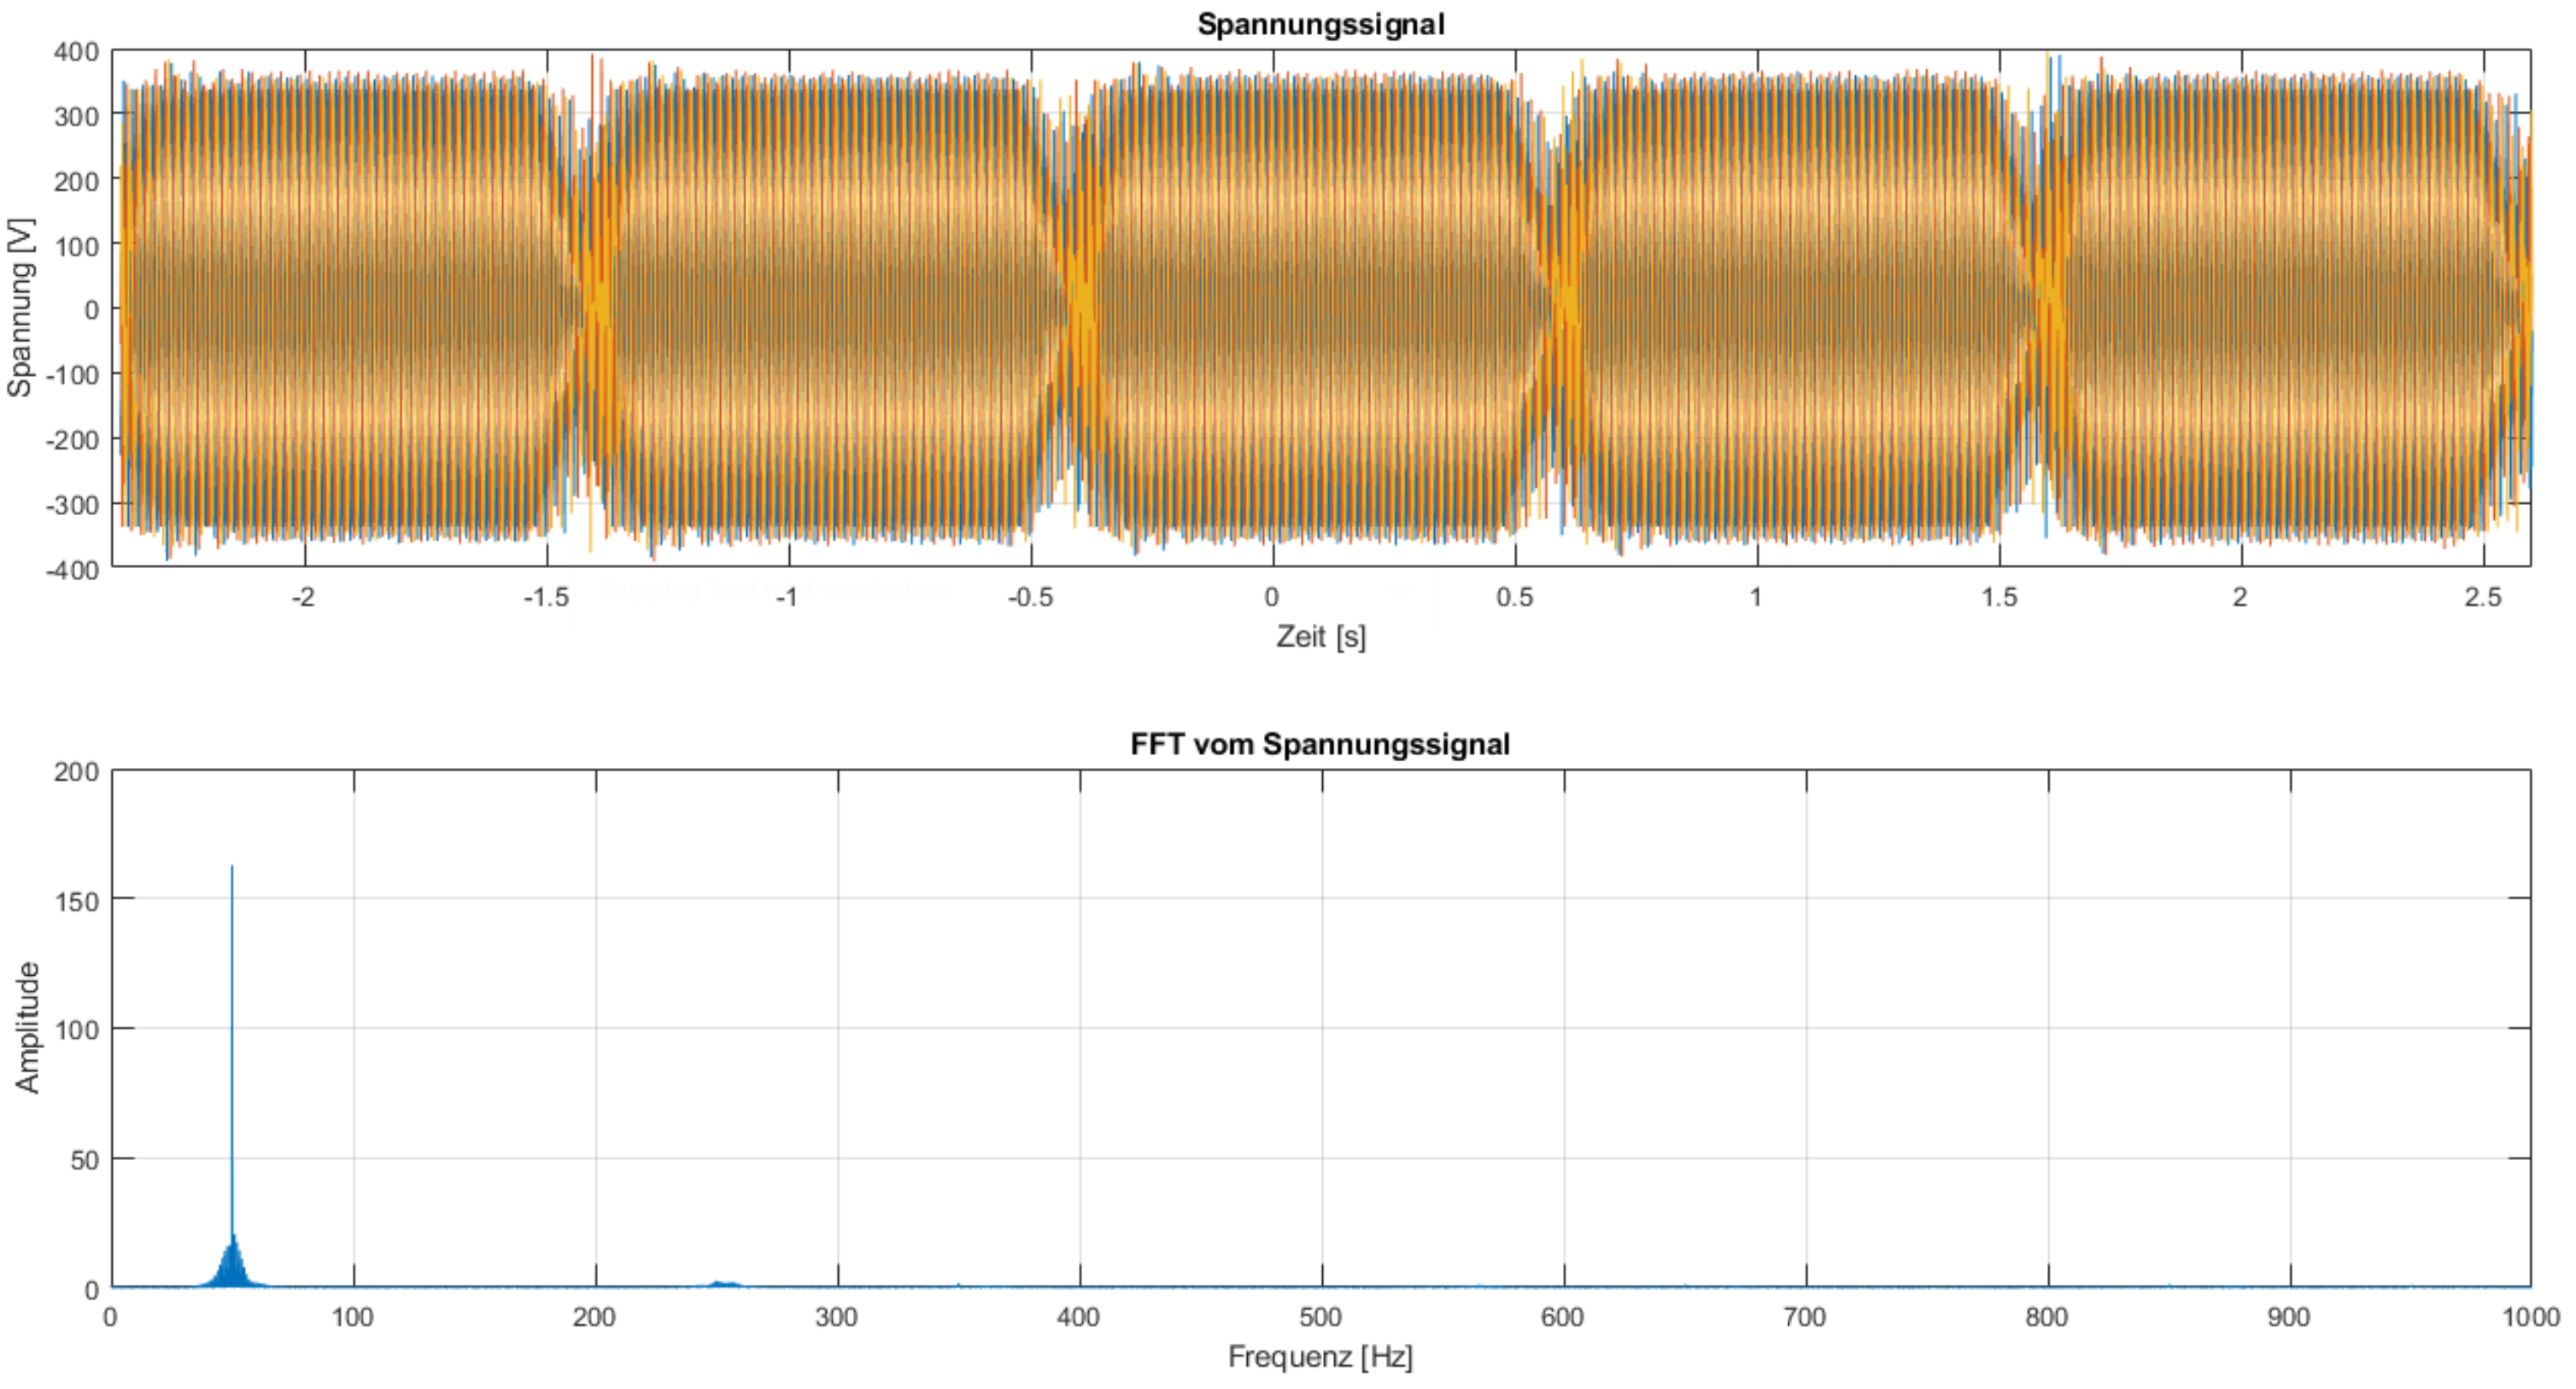
\includegraphics[width=\textwidth]{Messung_ASM_Schwing_0_8.png}	
	\caption{Messung mit Schwingungspaket 80\%}\label{fig:Mess_ASM_Schwing_0_8}
\end{figure}

\newpage
\subsubsection*{Auf- und Absteuern}
\begin{figure}[ht!]
	\centering
	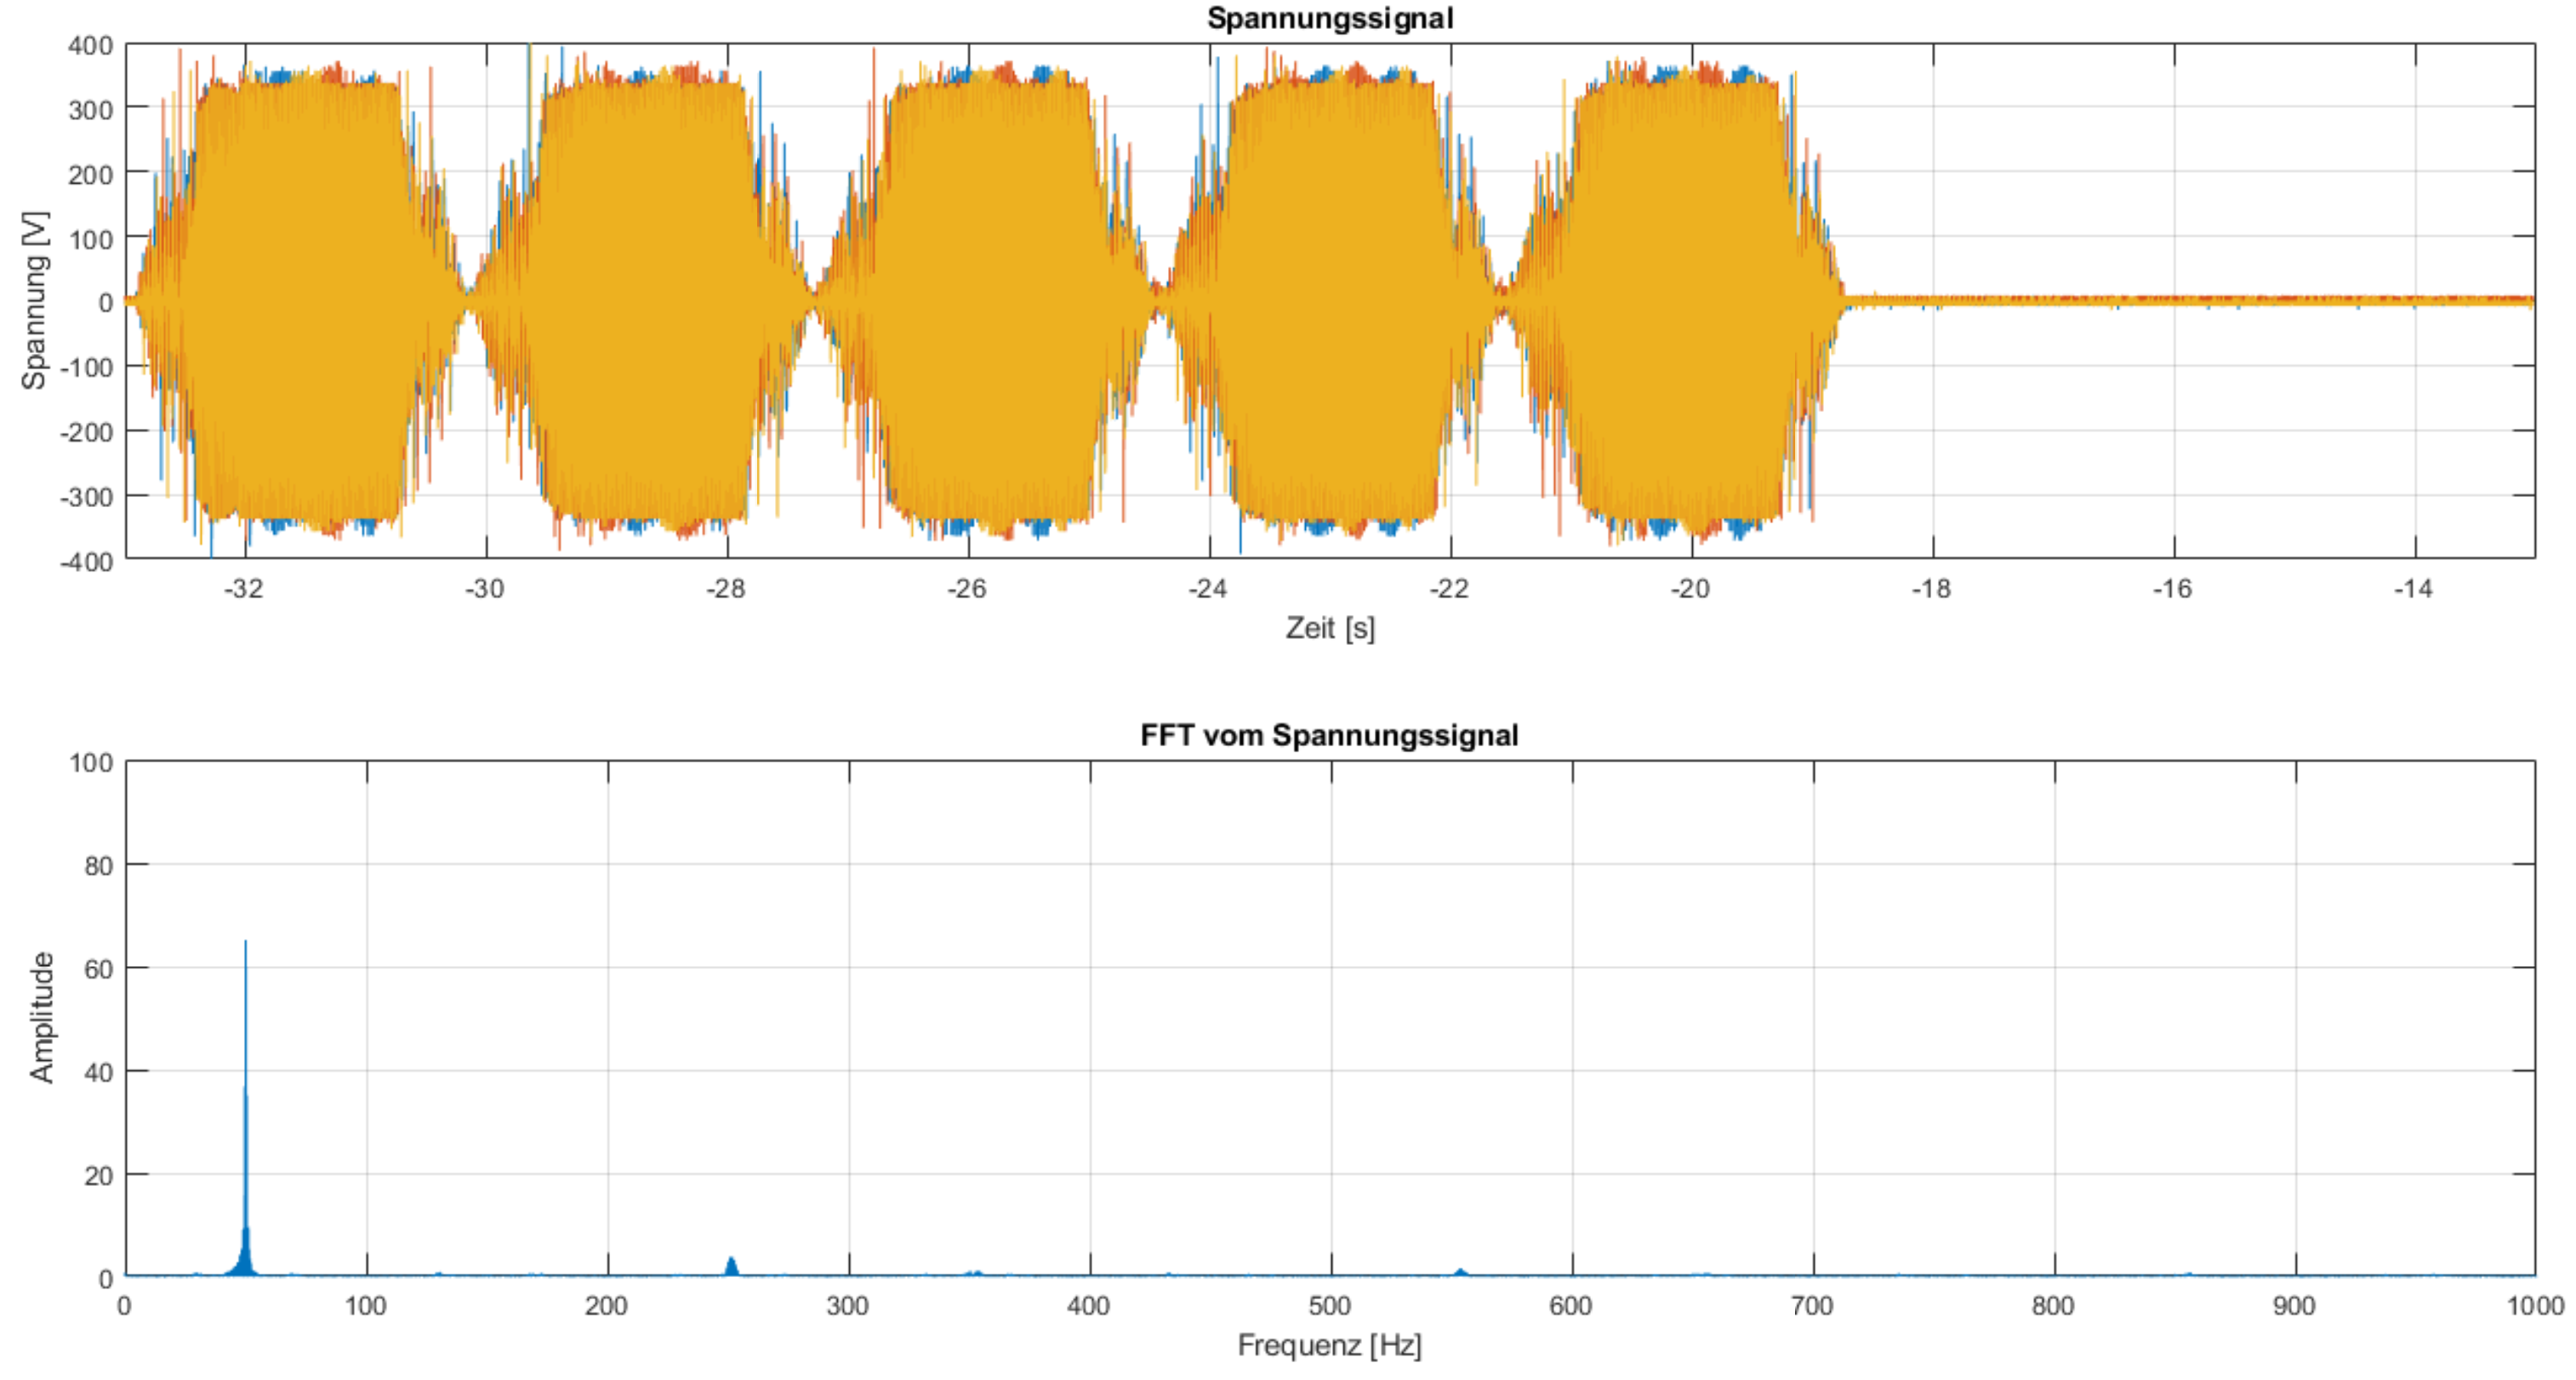
\includegraphics[width=\textwidth]{Messung_ASM_Sanft.png}	
	\caption{Messung mit Sanft Anlasser}\label{fig:Mess_ASM_Sanft}
\end{figure}


\newpage
\subsection{Spar-Variante für den Widerstand mit zwei Thyristoren}
\subsubsection*{Phasenanschnitt 60\textdegree}

\begin{figure}[ht!]
	\centering
	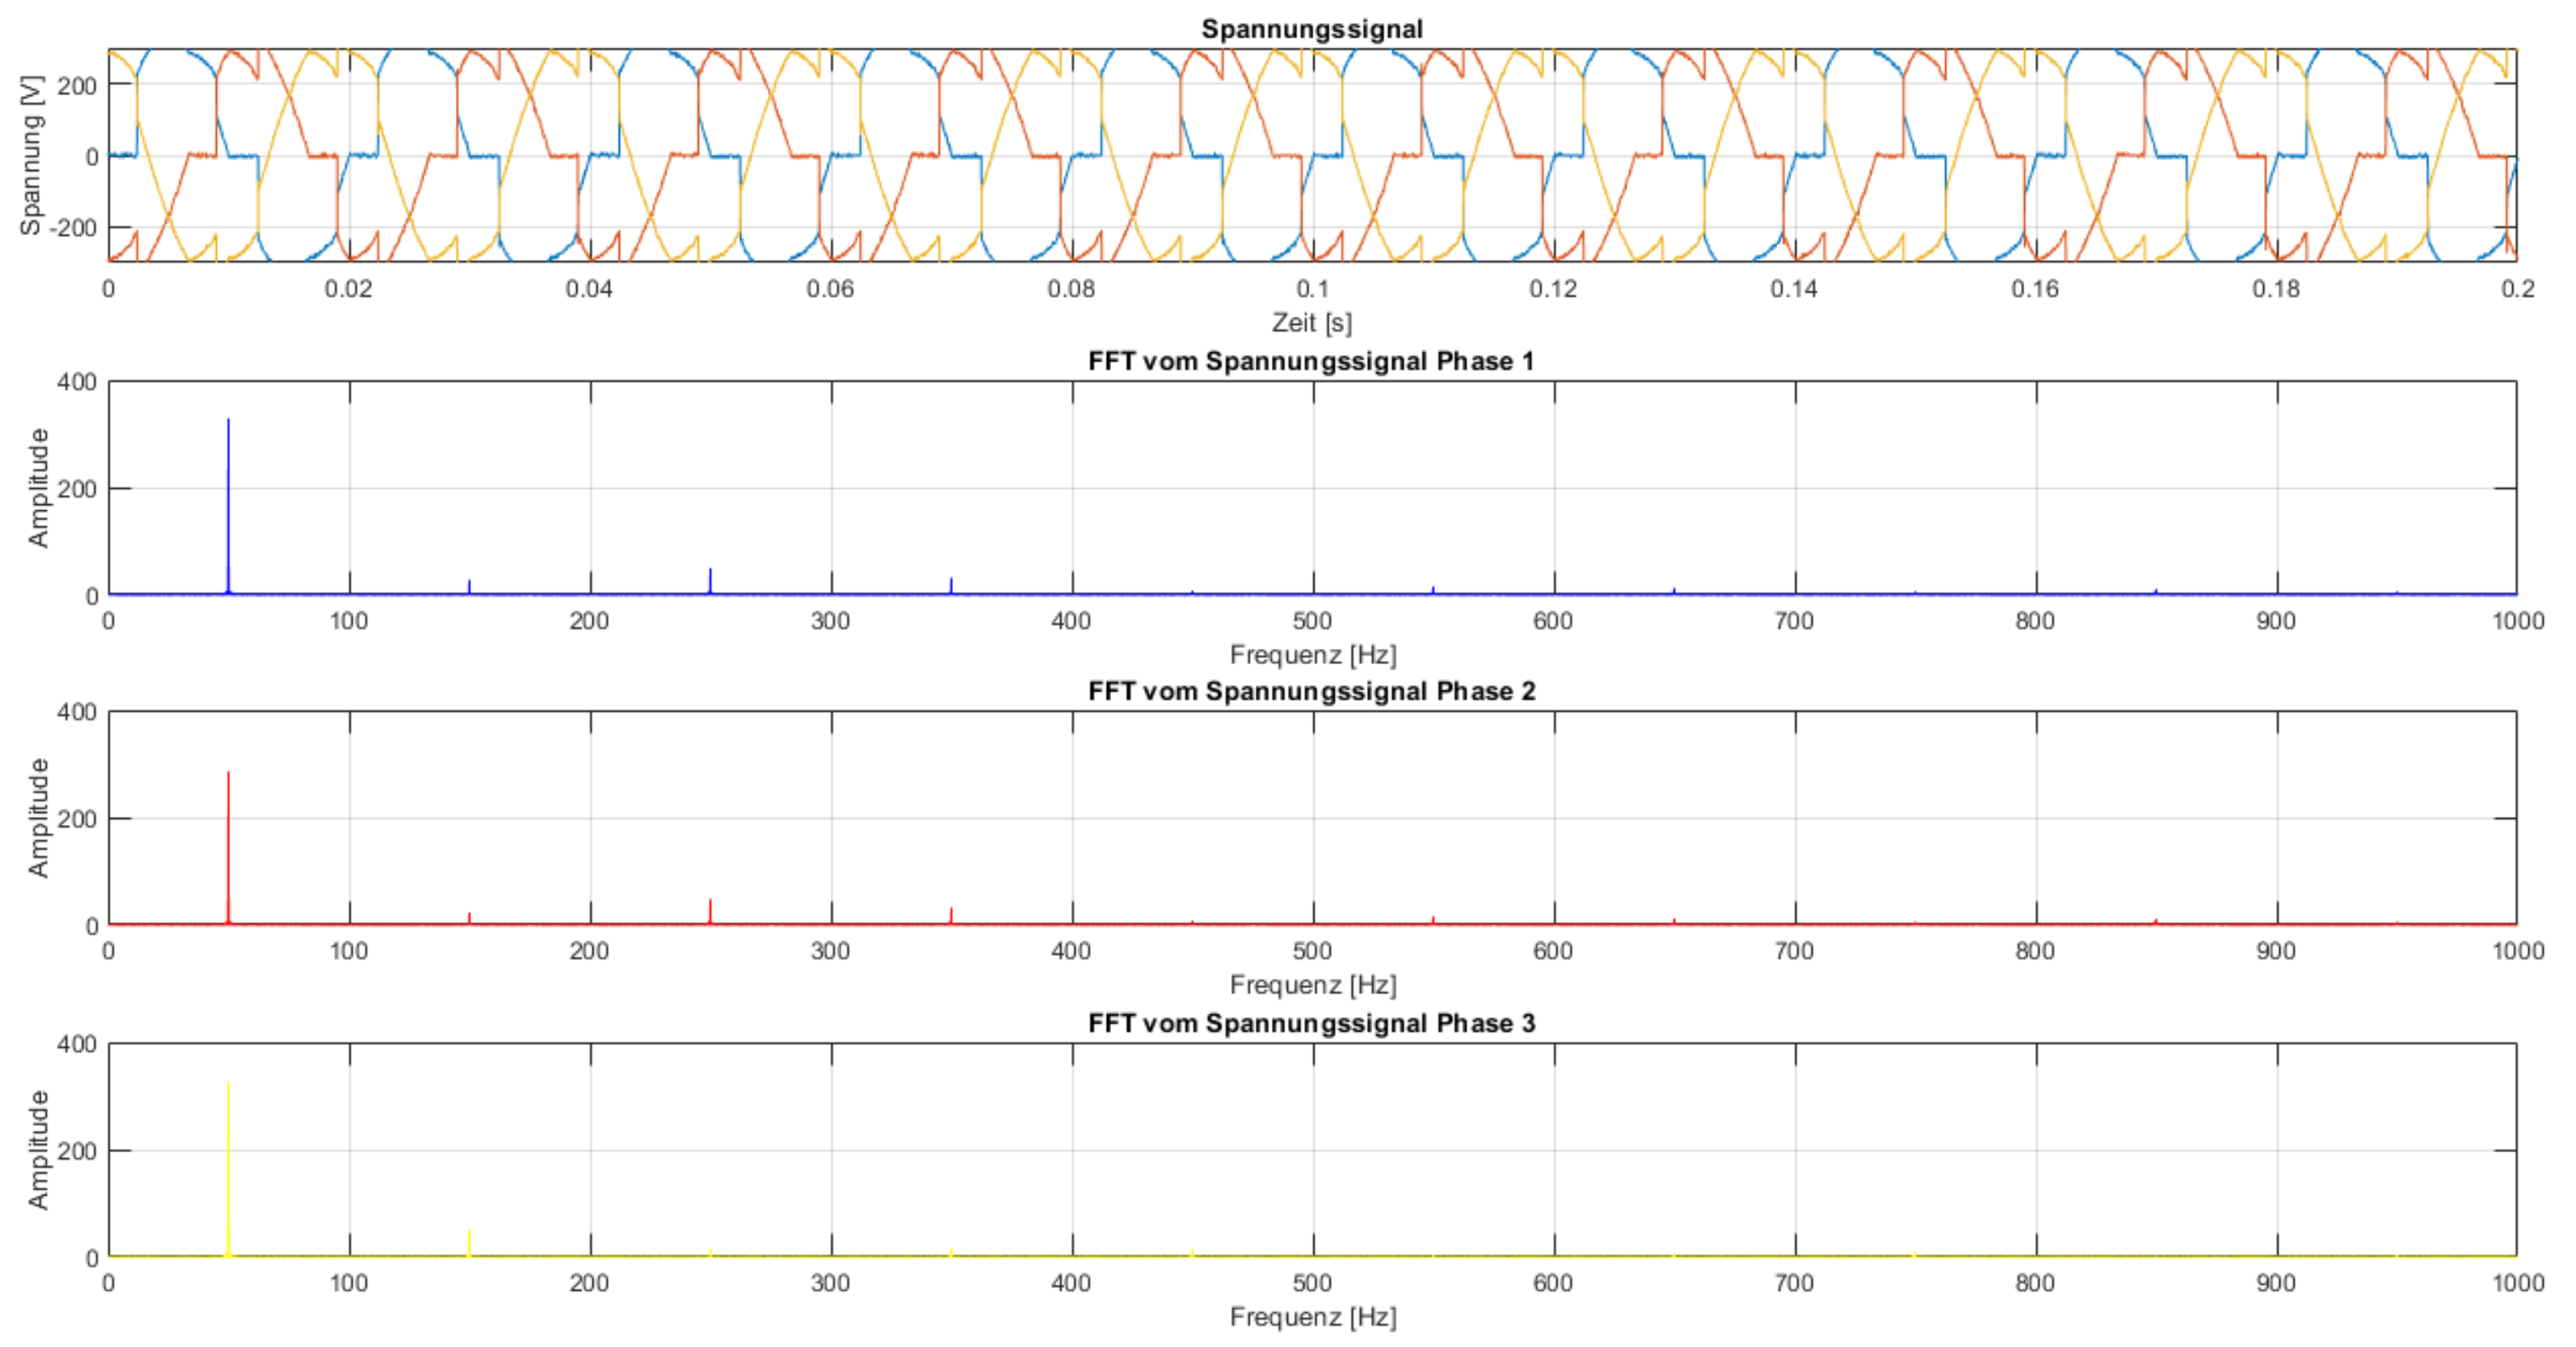
\includegraphics[width=\textwidth]{Mess_2Thyristoren_Widerstand_Phas_60.png}	
	\caption{Messung mit Phasenanschnitt 60\textdegree \hspace{0.02cm} und zwei Thyristoren}\label{fig:Mess_2Thyristoren_Phas_60grad}
\end{figure}

\newpage
\subsubsection*{Phasenanschnitt 90\textdegree}

\begin{figure}[ht!]
	\centering
	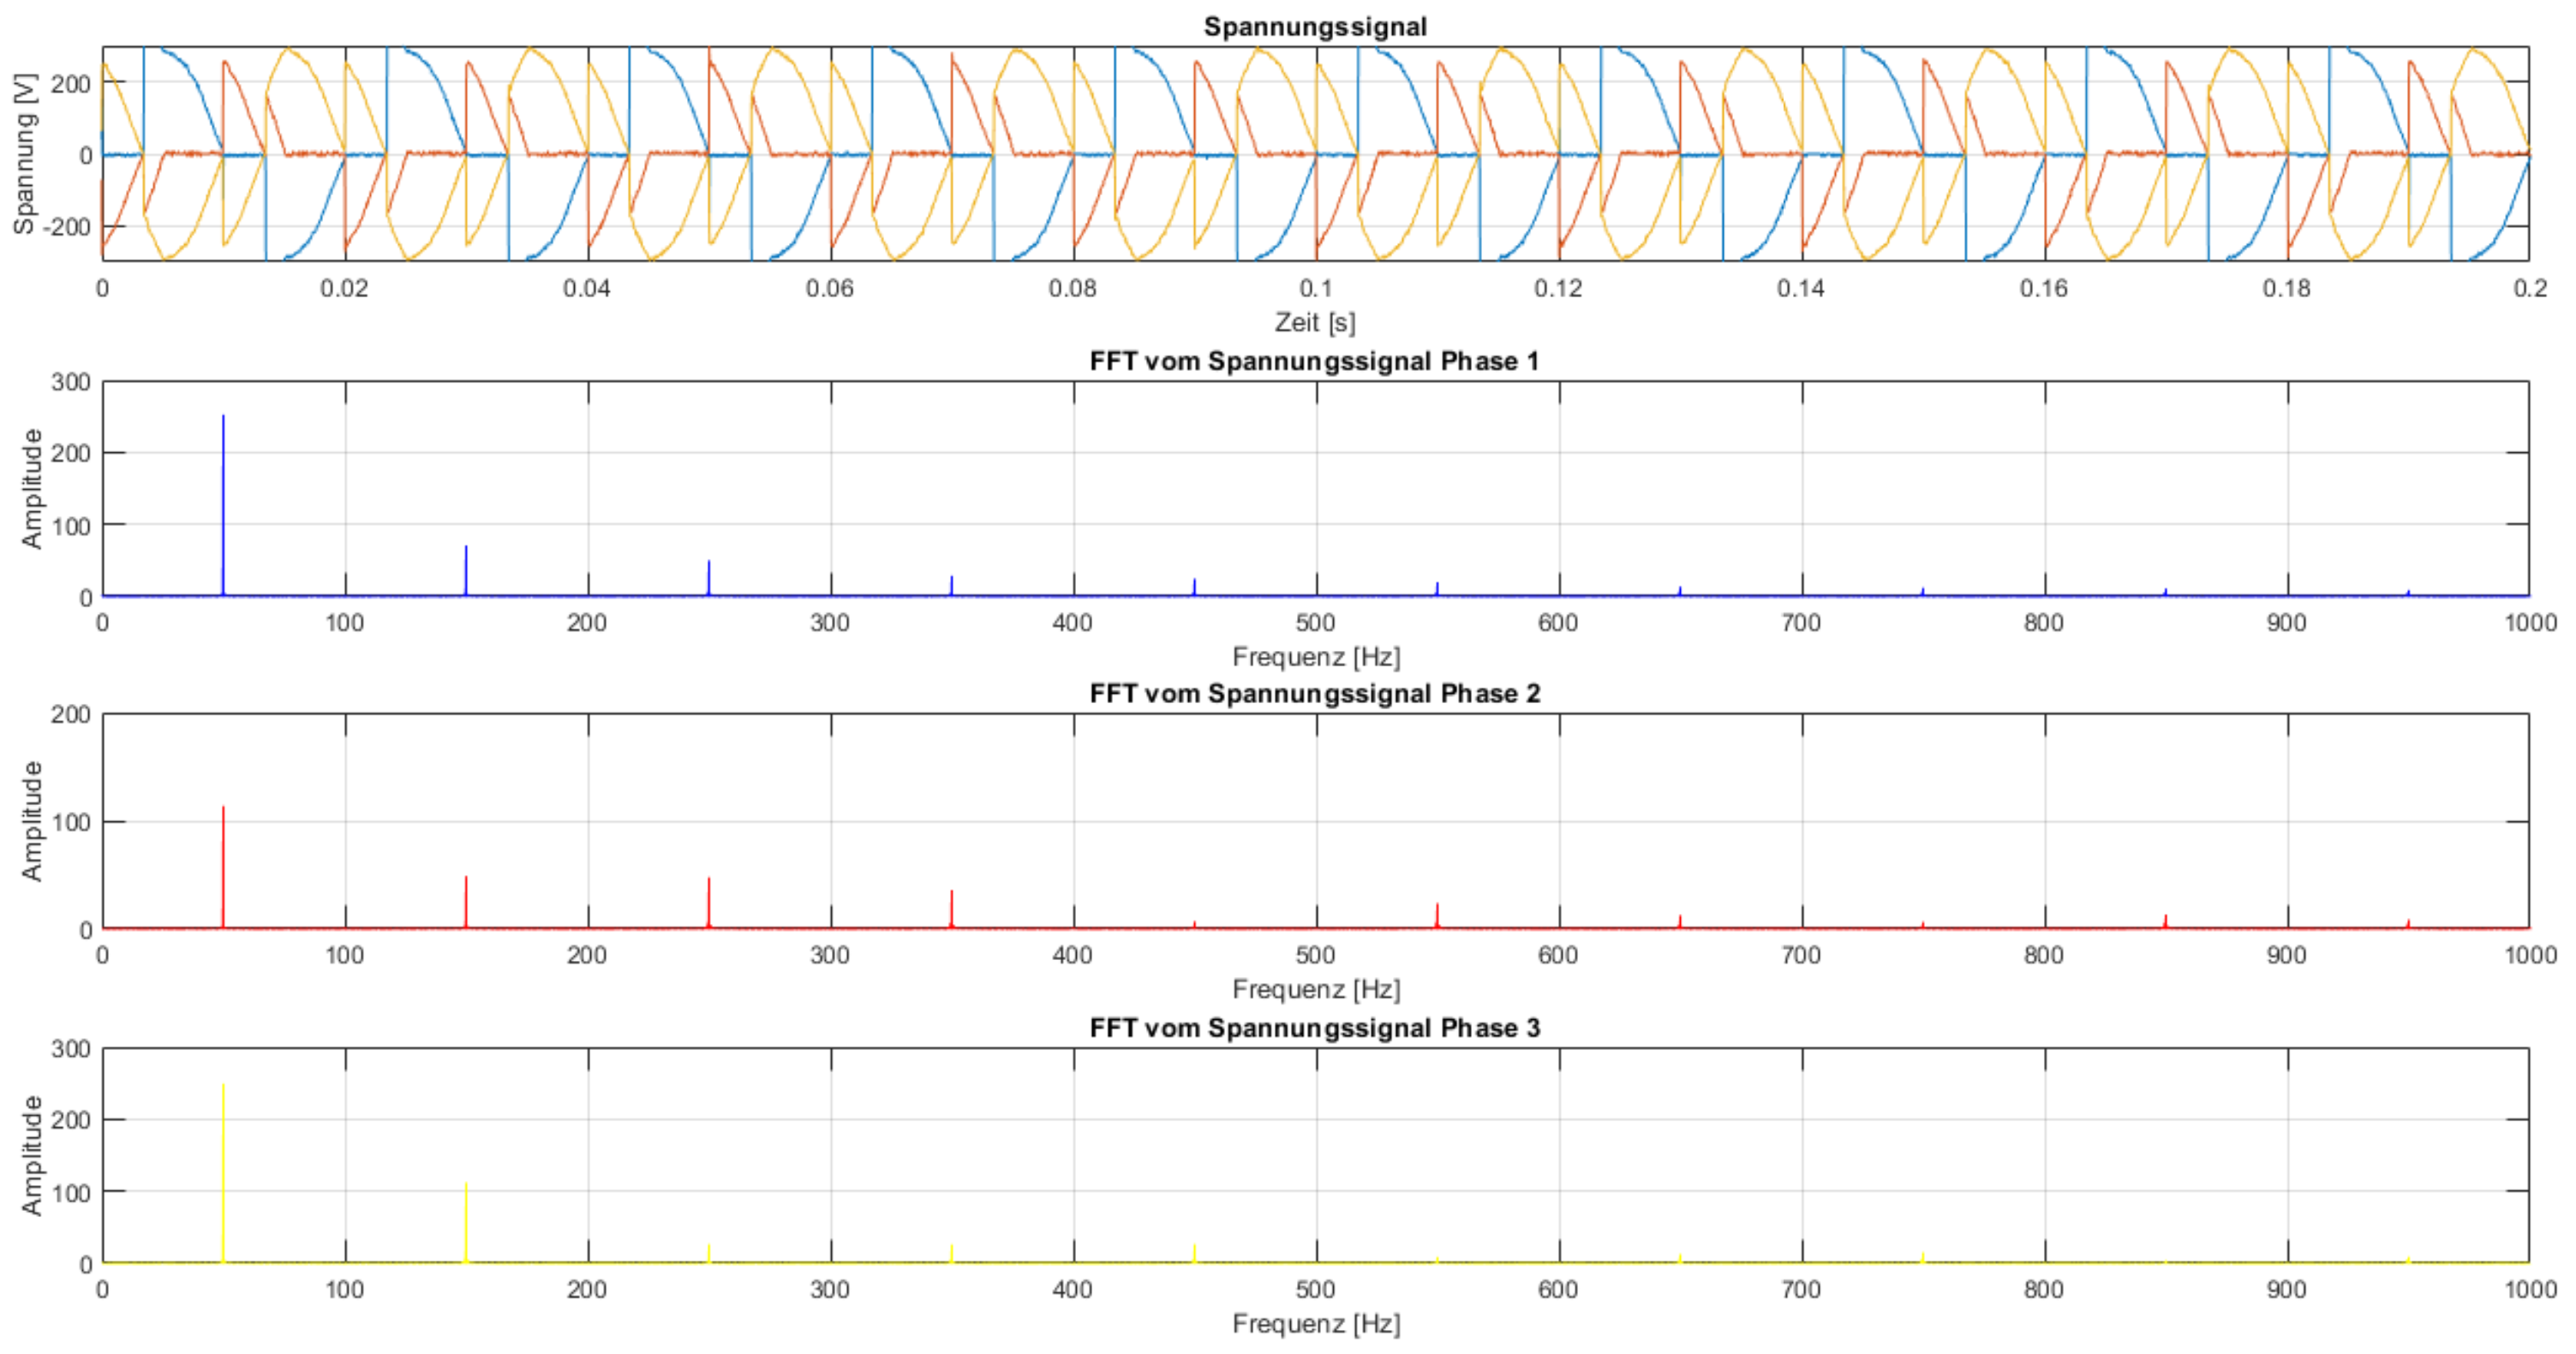
\includegraphics[width=\textwidth]{Mess_2Thyristoren_Widerstand_Phas_90.png}	
	\caption{Messung mit Phasenanschnitt 90\textdegree \hspace{0.02cm} und zwei Thyristoren}\label{fig:Mess_2Thyristoren_Phas_90grad}
\end{figure}

\newpage
\subsubsection*{Schwingungspaketsteuerung 50\%}

\begin{figure}[ht!]
	\centering
	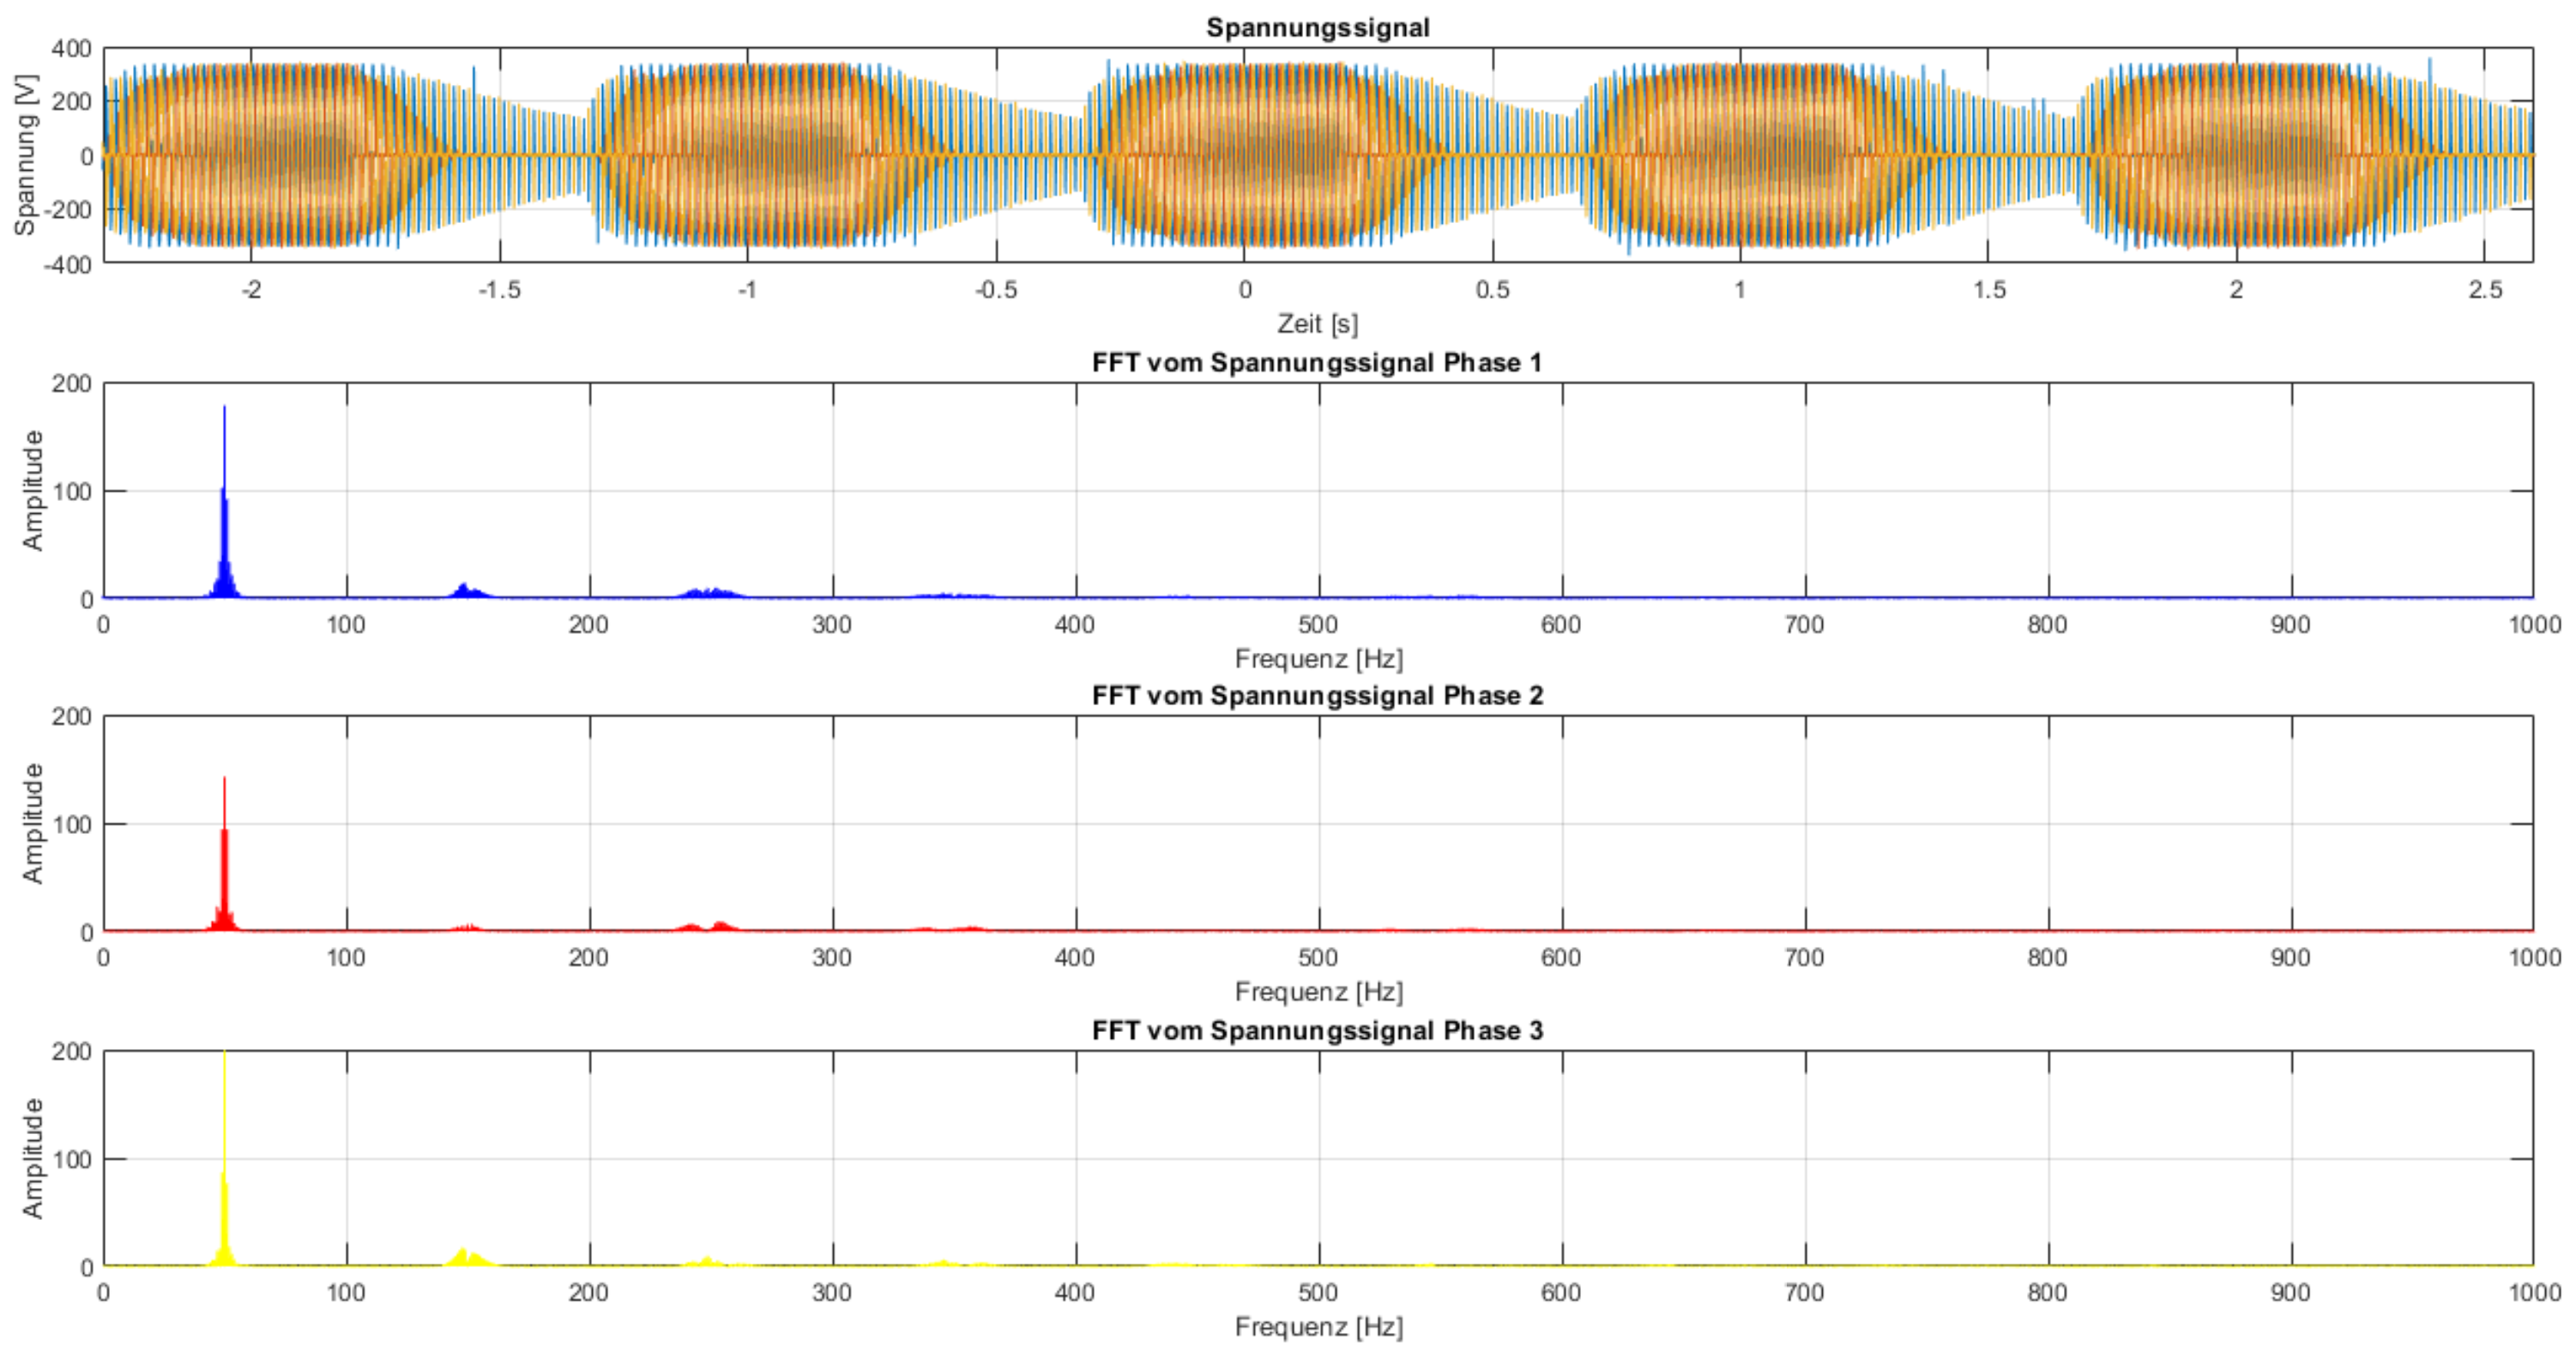
\includegraphics[width=\textwidth]{Mess_2Thyristoren_Widerstand_Schwing_05.png}	
	\caption{Messung mit Schwingungspaket 50\% und zwei Thyristoren}\label{fig:Mess_2Thyristoren_Schwing_50}
\end{figure}

\newpage
\subsubsection*{Schwingungspaketsteuerung 80\%}

\begin{figure}[ht!]
	\centering
	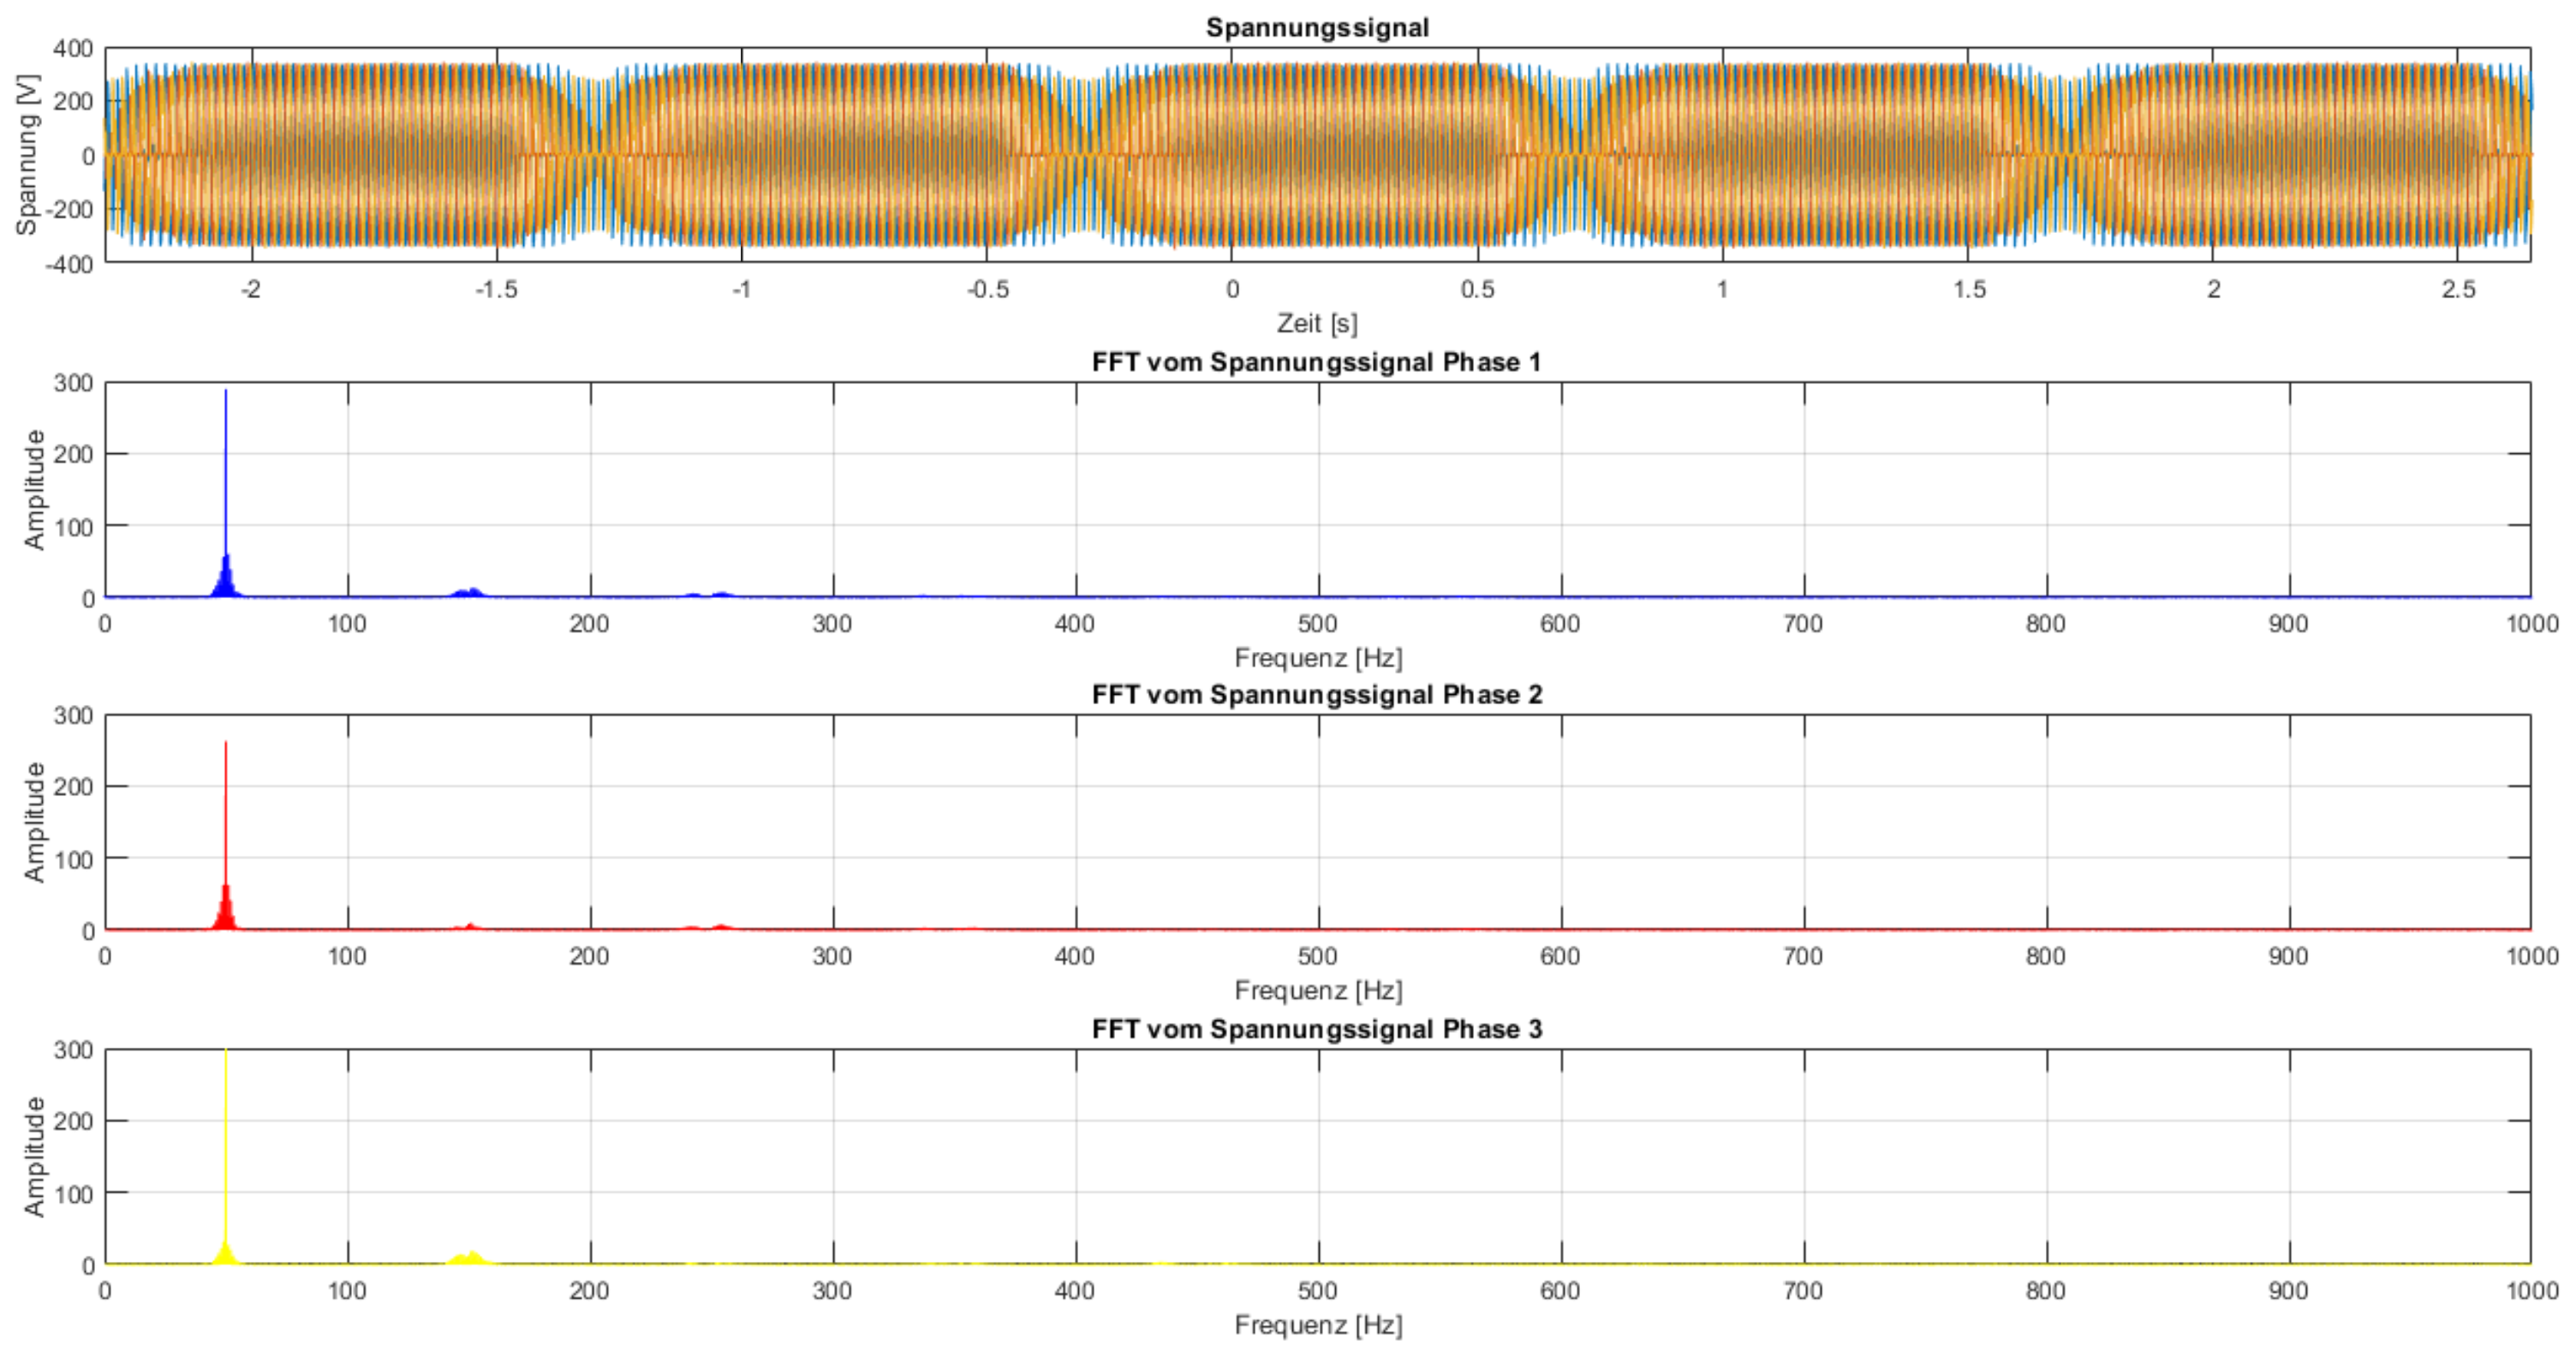
\includegraphics[width=\textwidth]{Mess_2Thyristoren_Widerstand_Schwing_08.png}	
	\caption{Messung mit Schwingungspaket 50\% und zwei Thyristoren}\label{fig:Mess_2Thyristoren_Schwing_80}	
\end{figure}


\newpage
\subsection{Spar-Variante für den Widerstand mit einem Thyristor}
\subsubsection*{Phasenanschnitt 60\textdegree}

\begin{figure}[ht]
	\centering
	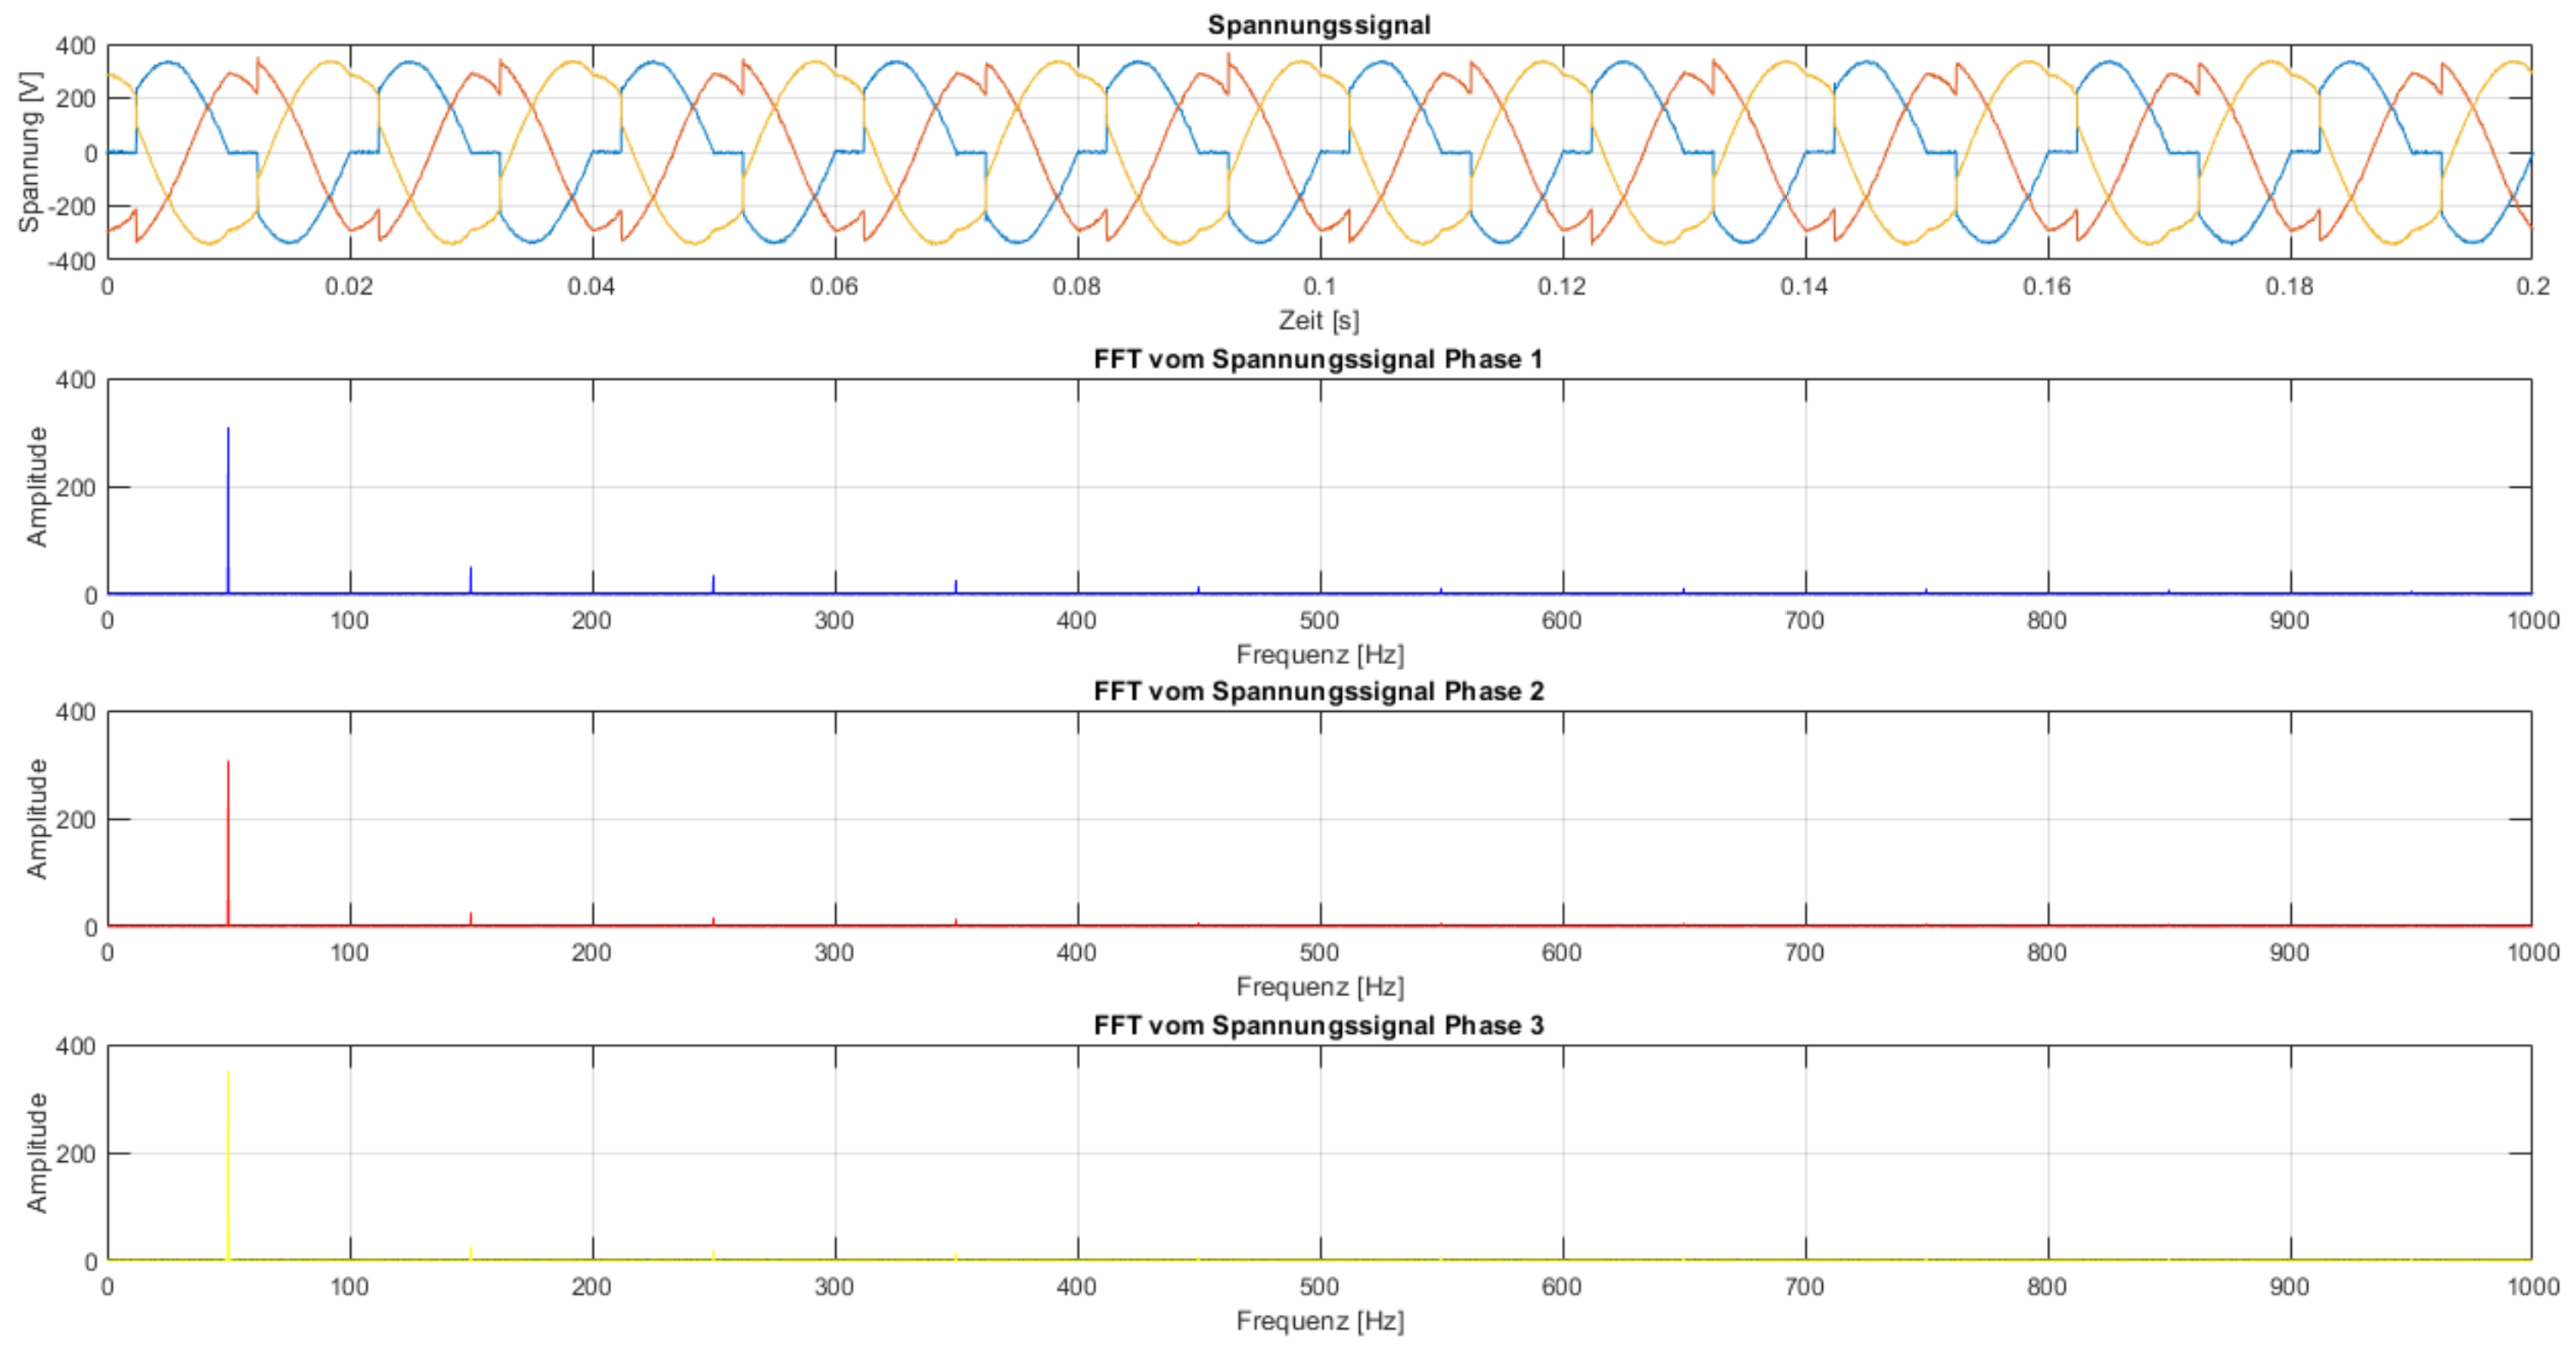
\includegraphics[width=\textwidth]{Mess_1Thyristor_Widerstand_Phas60.png}	
	\caption{Messung mit Phasenanschnitt 60\textdegree \hspace{0.02cm} und einem Thyristoren}\label{fig:Mess_1Thyristor_Phas_60grad}
\end{figure}


\subsubsection*{Phasenanschnitt 90\textdegree}

\begin{figure}[ht]
	\centering
	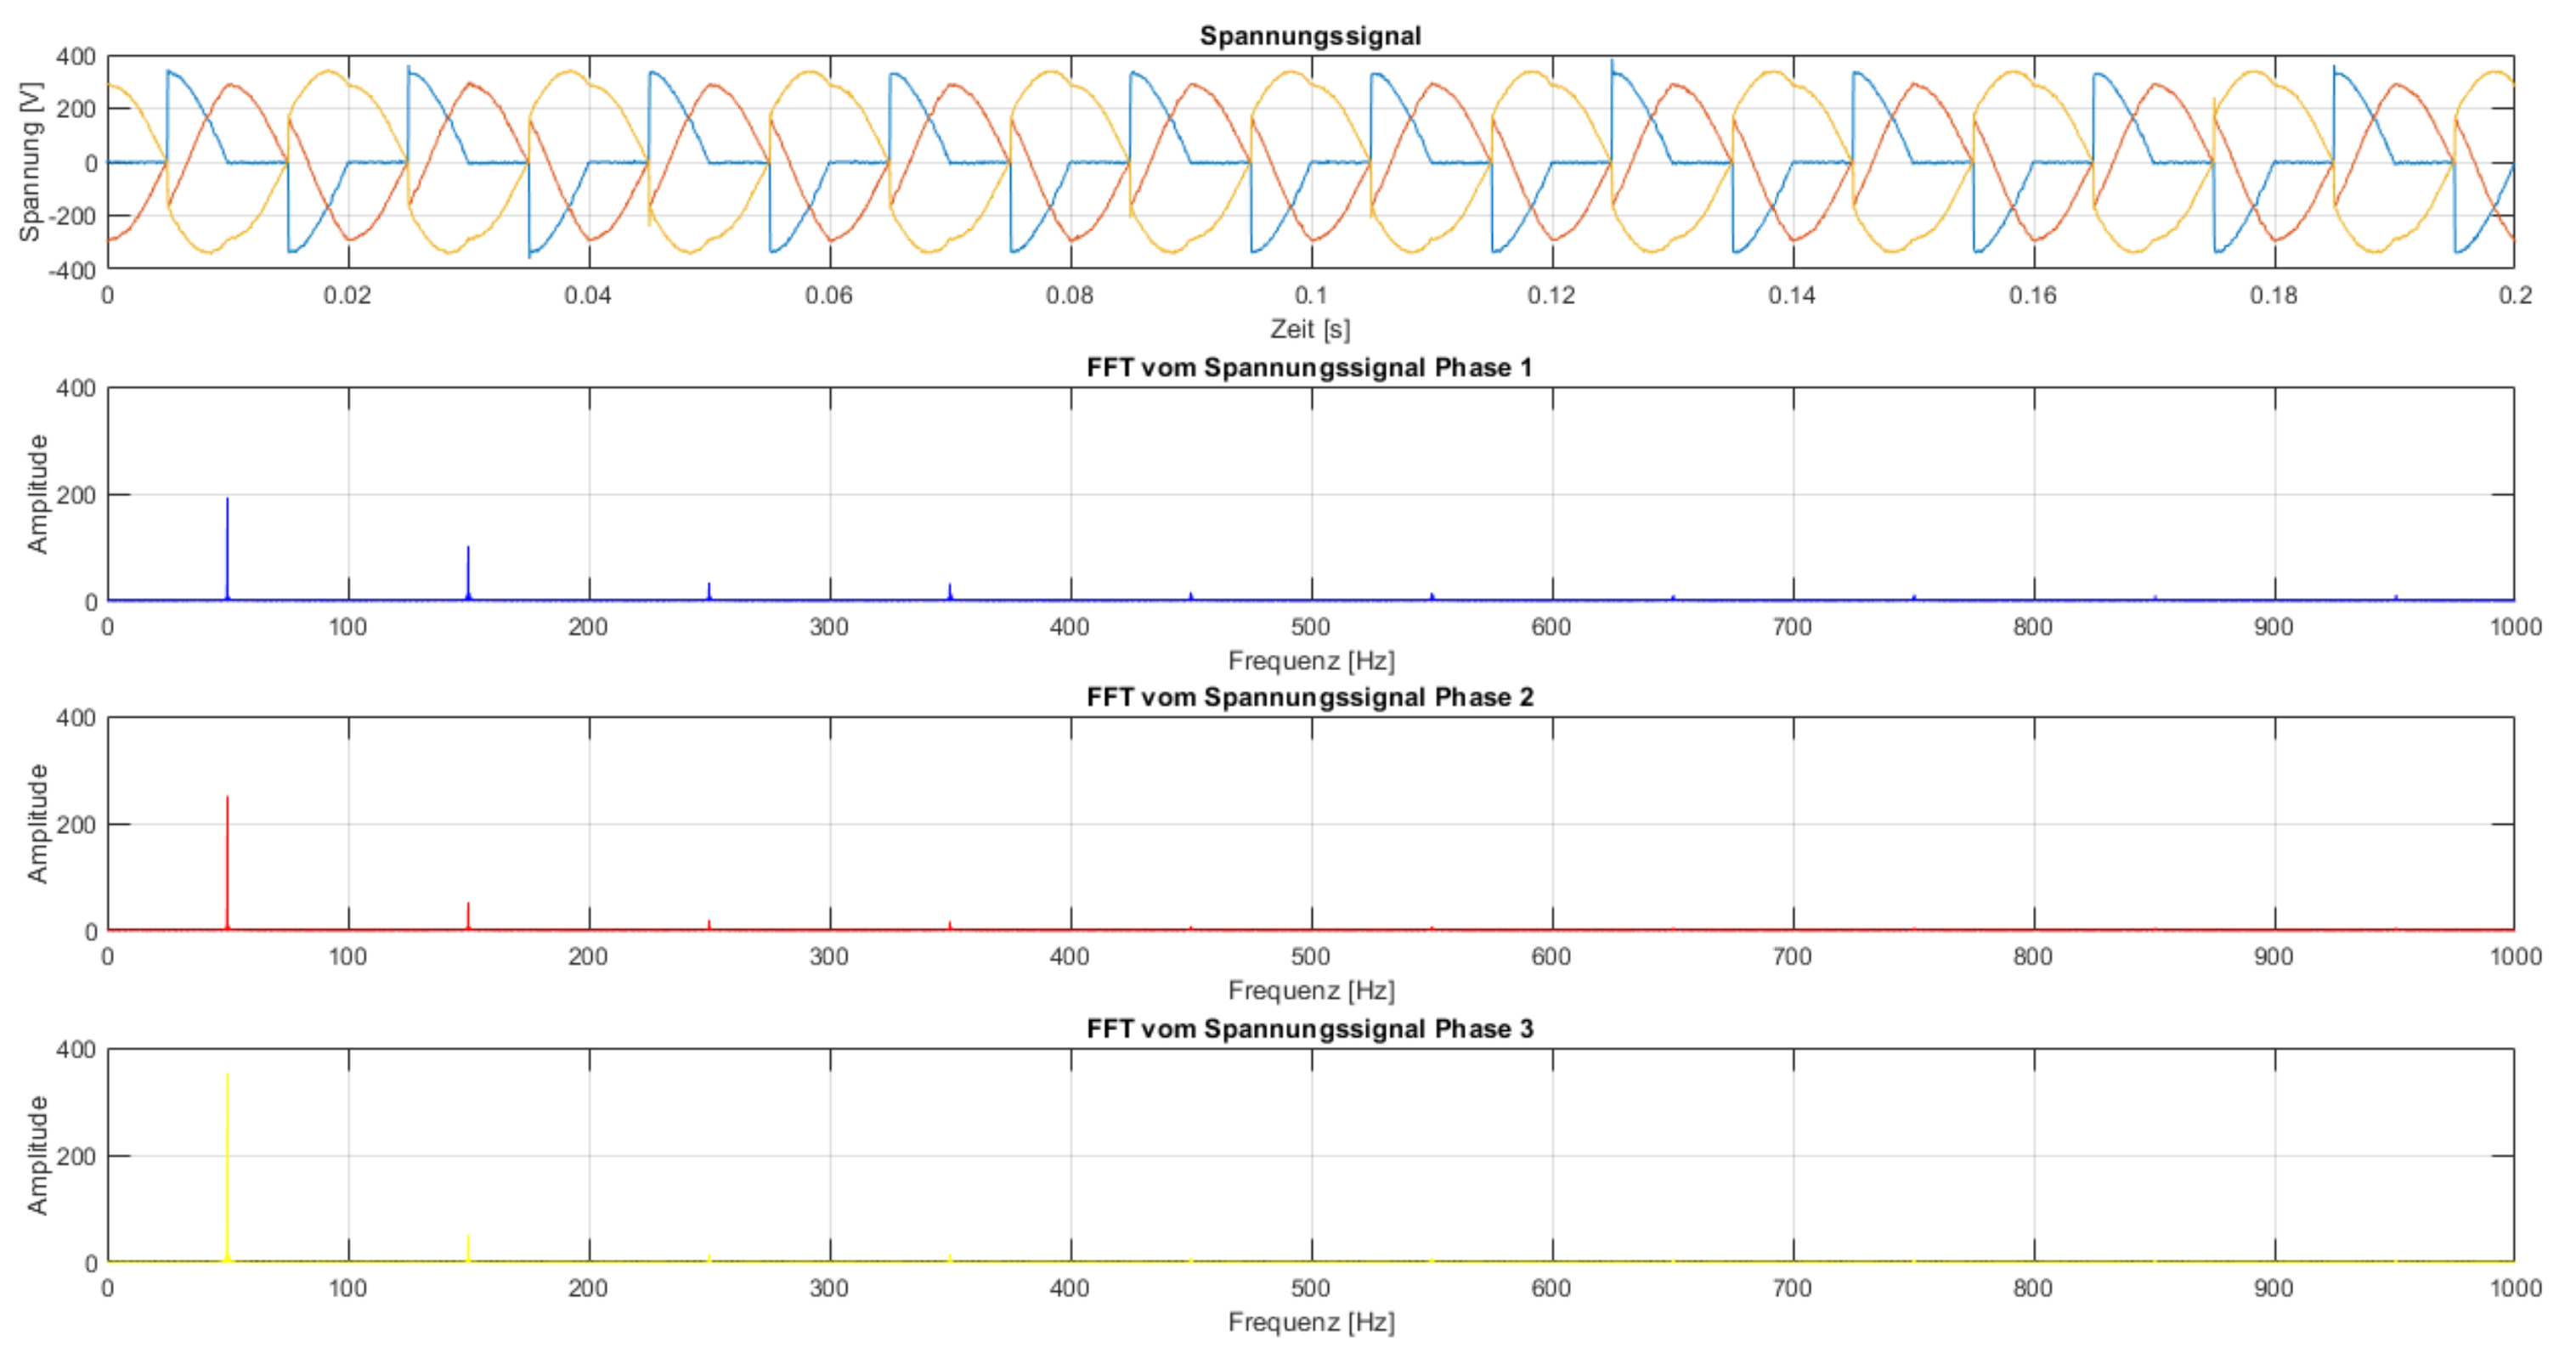
\includegraphics[width=\textwidth]{Mess_1Thyristor_Widerstand_Phas90.png}	
	\caption{Messung mit Phasenanschnitt 90\textdegree \hspace{0.02cm} und einem Thyristoren}\label{fig:Mess_1Thyristor_Phas_90grad}
\end{figure}


\subsubsection*{Schwingungspaketsteuerung 50\%}

\begin{figure}[ht]
	\centering
	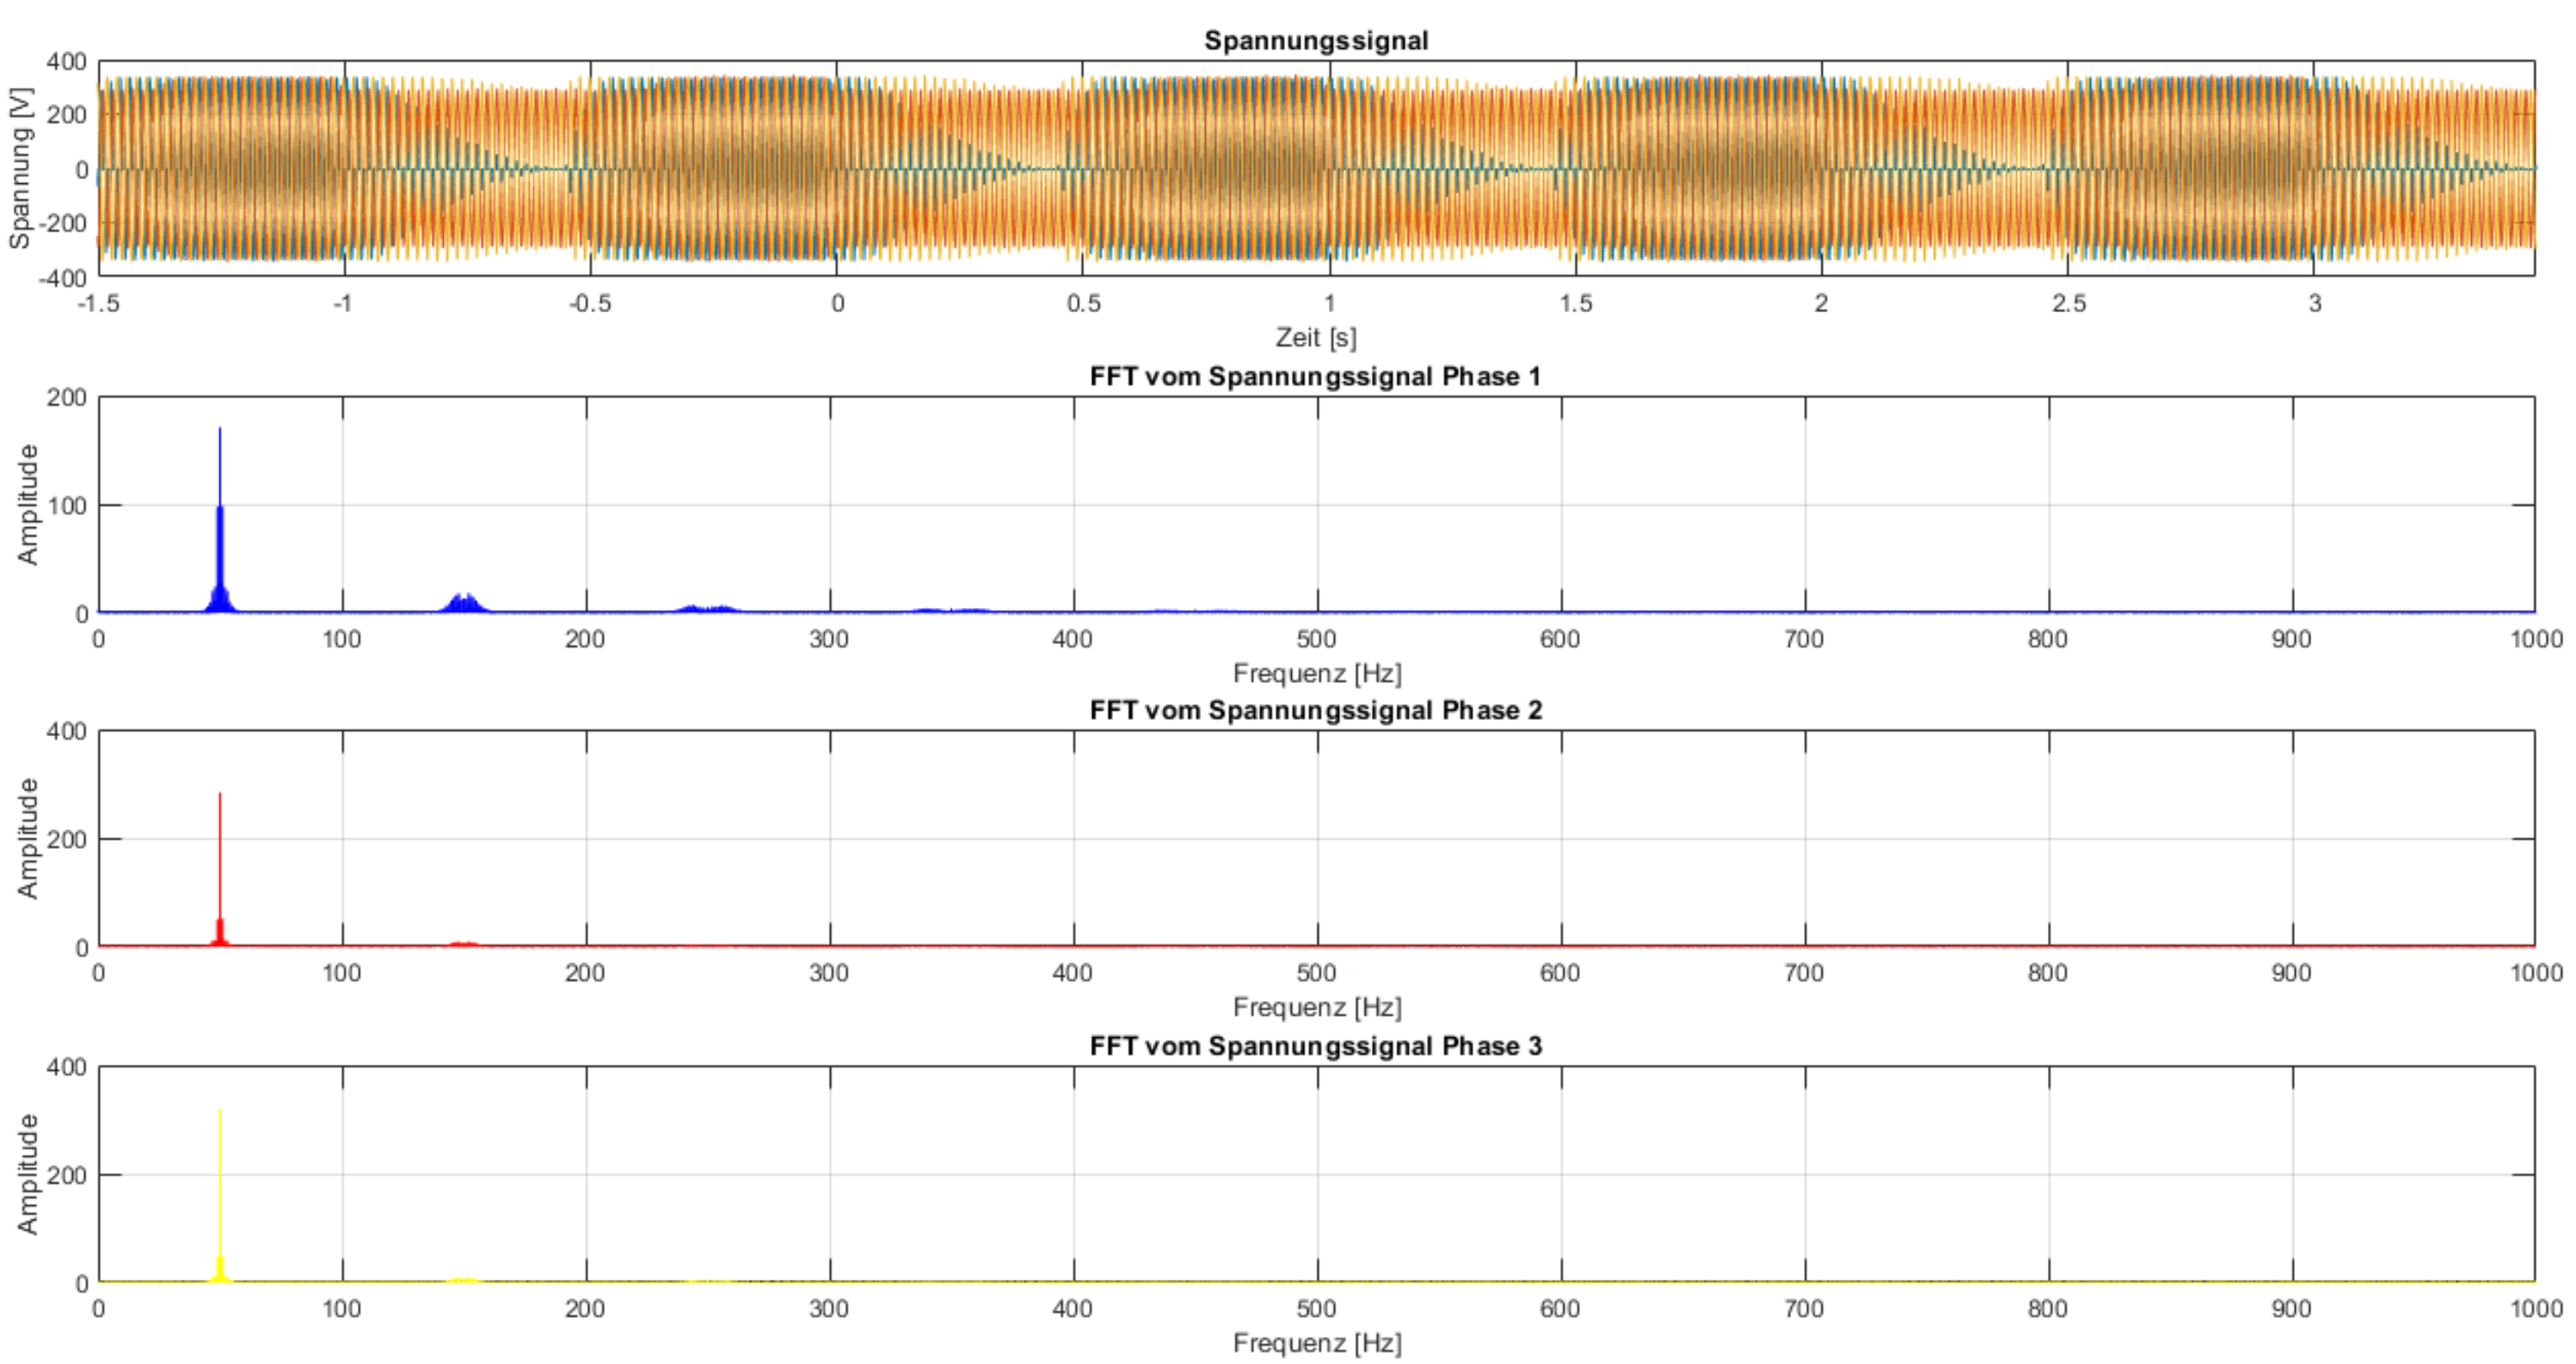
\includegraphics[width=\textwidth]{Mess_1Thyristor_Widerstand_Schwing_05.png}	
	\caption{Messung mit Schwingungspaket 50\% und einem Thyristoren}\label{fig:Mess_1Thyristor_Schwing_50}
\end{figure}


\subsubsection*{Schwingungspaketsteuerung 80\%}

\begin{figure}[ht]
	\centering
	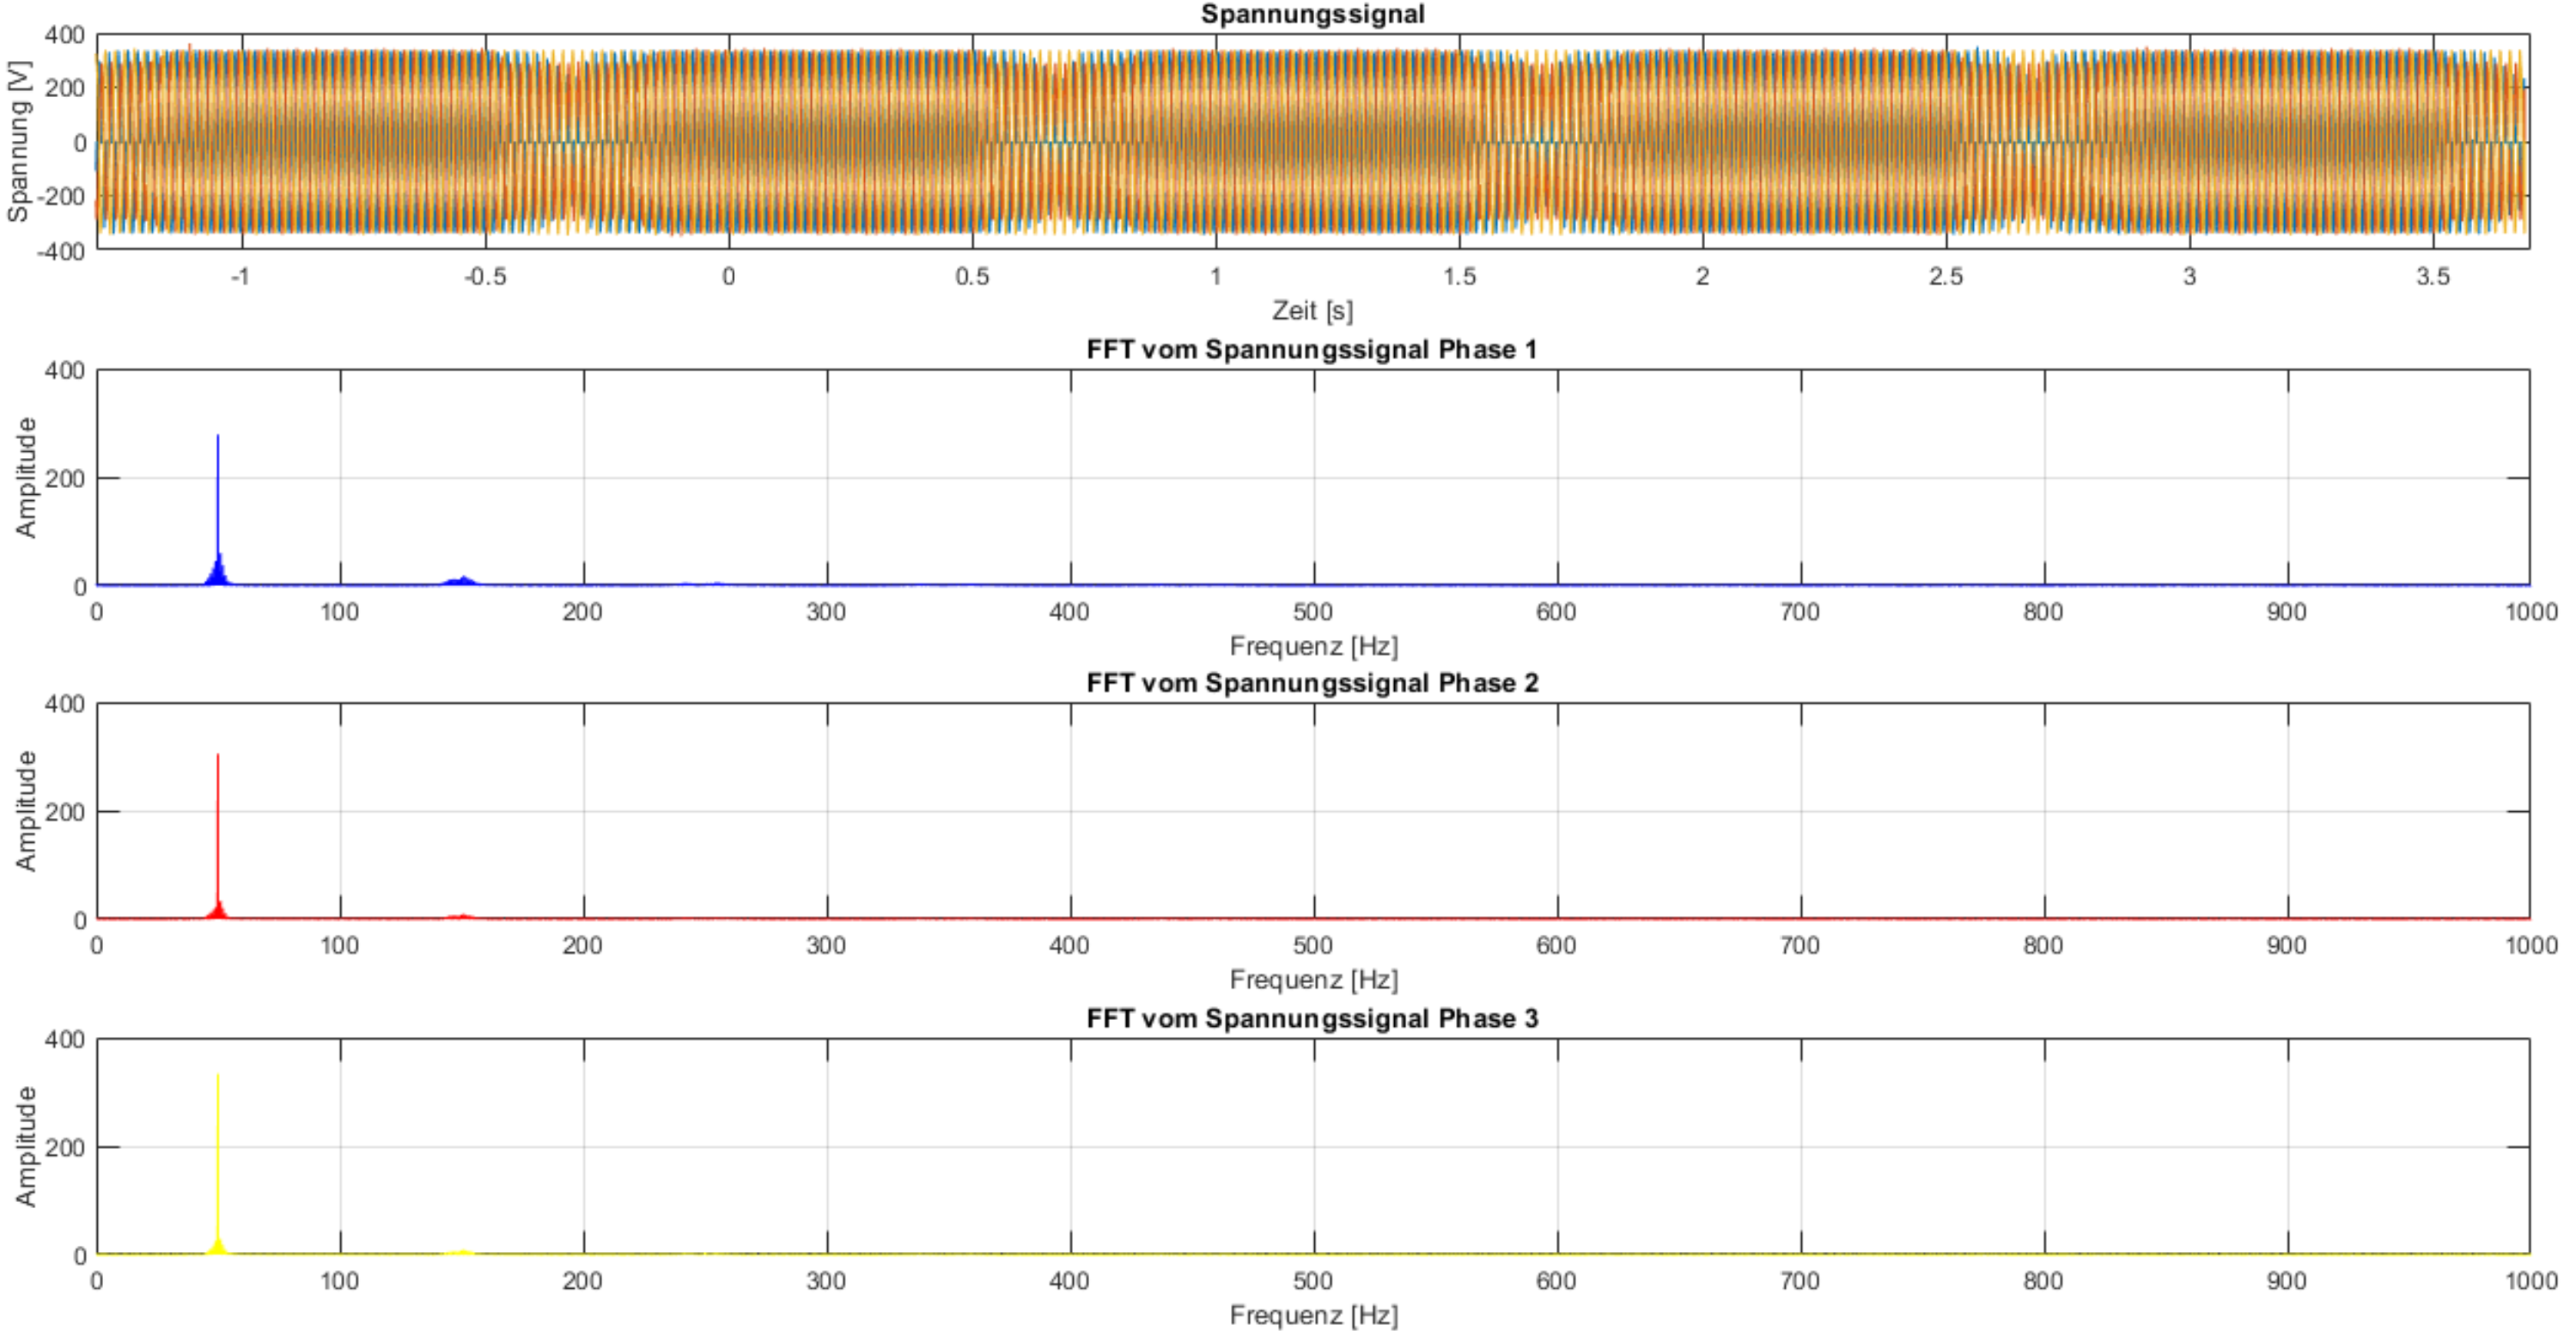
\includegraphics[width=\textwidth]{Mess_1Thyristor_Widerstand_Schwing_08.png}	
	\caption{Messung mit Schwingungspaket 50\% und einem Thyristoren}\label{fig:Mess_1Thyristoren_Schwing_80}	
\end{figure}


\subsubsection*{Auf- und Absteuern}

\begin{figure}[ht]
	\centering
	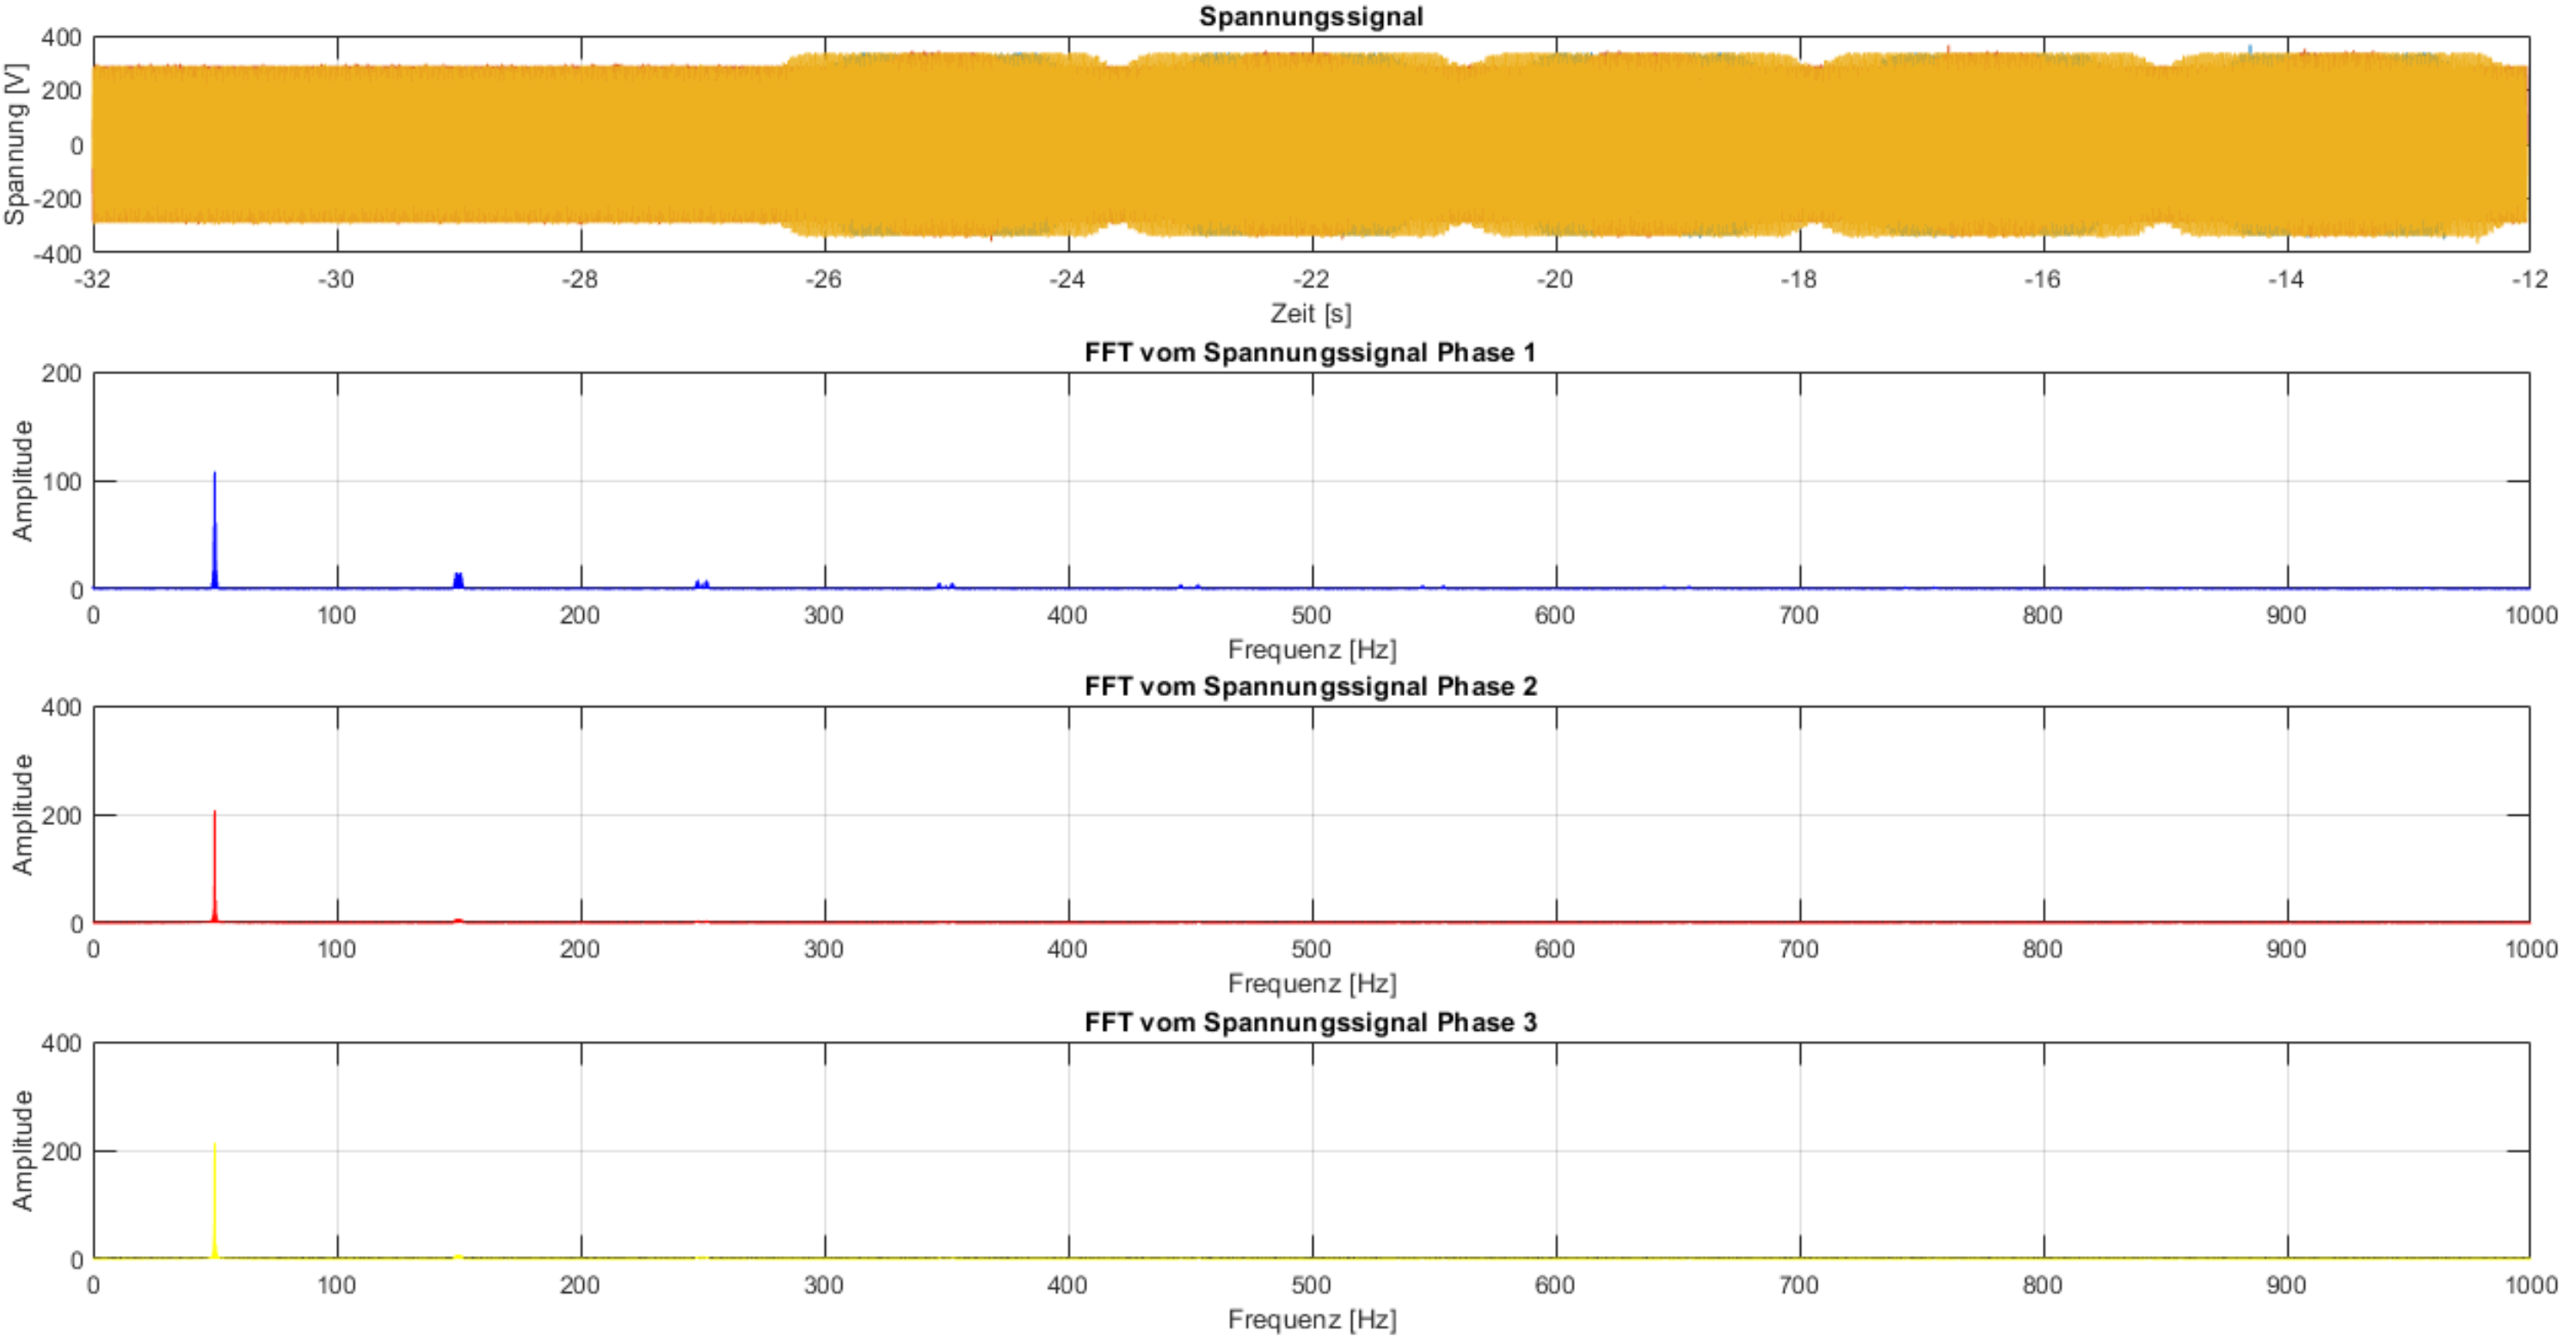
\includegraphics[width=\textwidth]{Mess_1Thyristor_Widerstand_AufAb.png}	
	\caption{Messung mit Auf- und Absteuern und einem Thyristoren}\label{Mess_1Thyristoren_Widerstand_AufAbFahren}	
\end{figure}


\subsubsection*{Langsames Auf- und Absteuern}

\begin{figure}[ht]
	\centering
	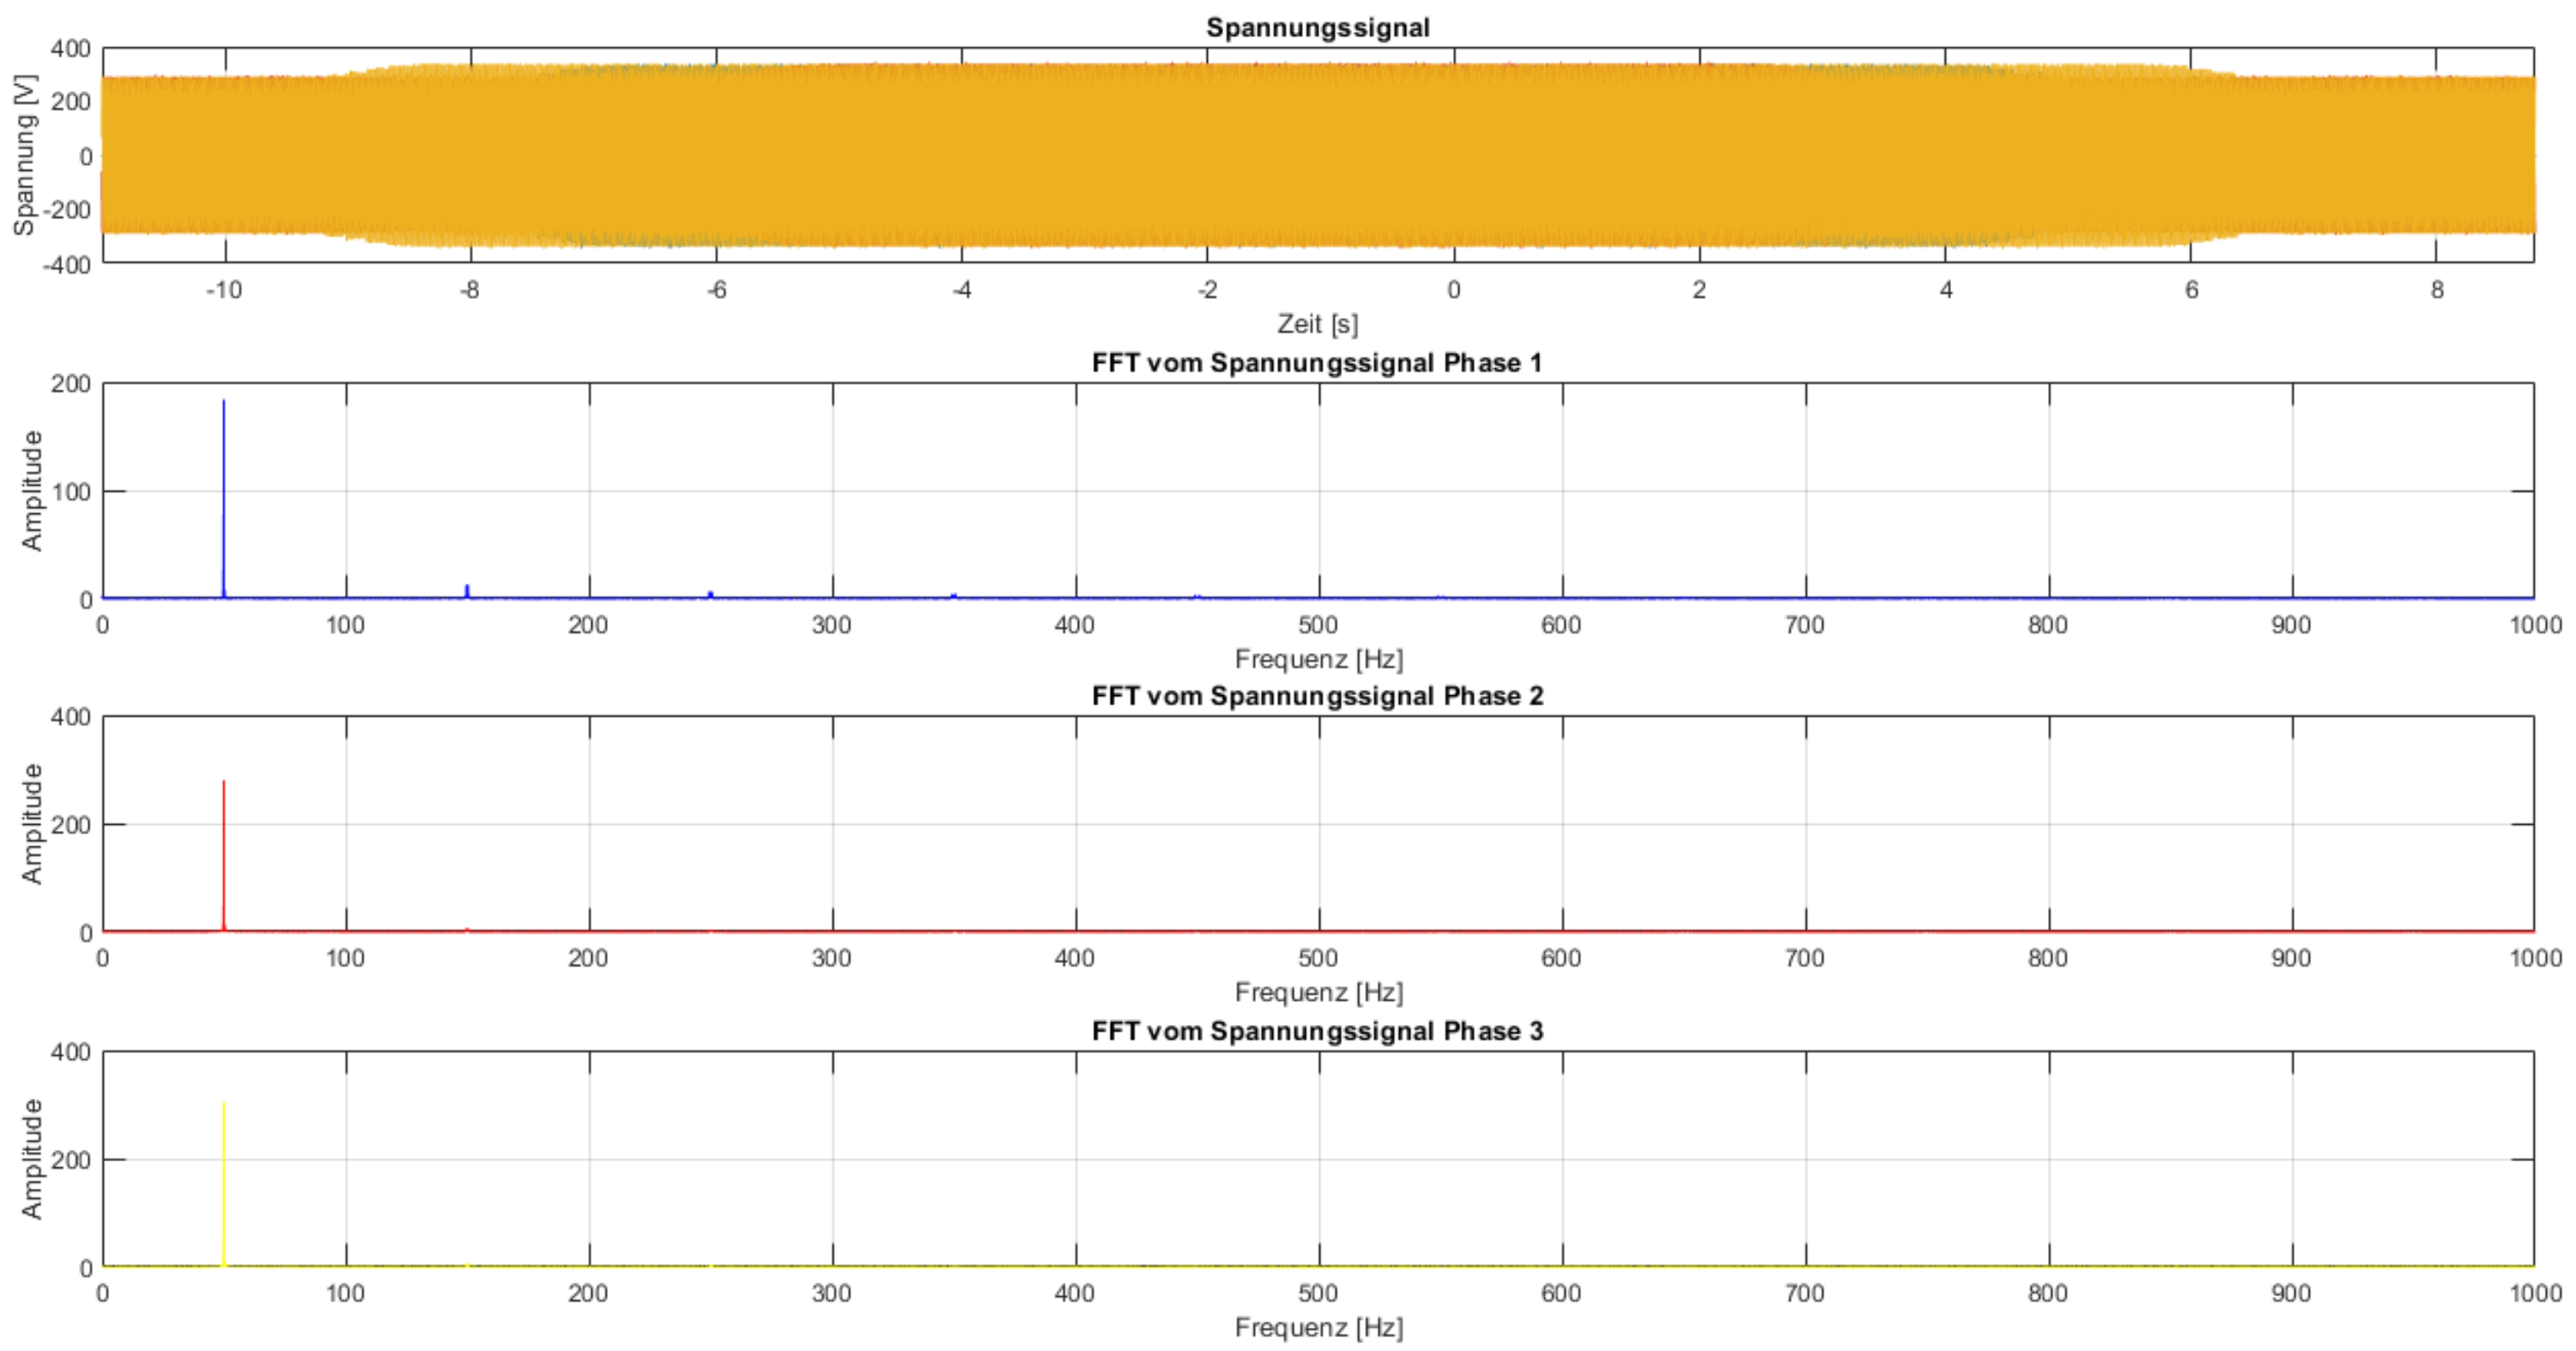
\includegraphics[width=\textwidth]{Mess_1Thyristor_Widerstand_AufAb_langsam.png}	
	\caption{Messung mit dem langsamen Auf- und Absteuern und einem Thyristoren}\label{Mess_1Thyristoren_Widerstand_AufAbFahren_langsam}	
\end{figure}

\end{appendix}


